% Created 2023-05-01 Mon 09:21
\documentclass[9pt, b5paaper]{book}
\usepackage{xeCJK}
\usepackage[T1]{fontenc}
\usepackage[scaled]{beraserif}
\usepackage[scaled]{berasans}
\usepackage[scaled]{beramono}
\usepackage{graphicx}
\usepackage{xcolor}
\usepackage{multirow}
\usepackage{multicol}
\usepackage{float}
\usepackage{textcomp}
\usepackage{geometry}
\geometry{left=1.2cm,right=1.2cm,top=1.5cm,bottom=1.2cm}
\usepackage{algorithm}
\usepackage{algorithmic}
\usepackage{latexsym}
\usepackage{natbib}
\usepackage{minted}
\newminted{common-lisp}{fontsize=\footnotesize}
\usepackage[xetex,colorlinks=true,CJKbookmarks=true,linkcolor=blue,urlcolor=blue,menucolor=blue]{hyperref} 
\author{Heyan Huang}
\date{\today}
\title{dp}
\hypersetup{
  pdfkeywords={},
  pdfsubject={},
  pdfcreator={Emacs 28.2 (Org mode 8.2.7c)}}
\begin{document}

\maketitle
\tableofcontents


\chapter{Dynamic Programming, 动态规划}
\label{sec-1}
\section{第二次仍不会的题号记这里}
\label{sec-1-1}
\begin{itemize}
\item 1872 (stone game 8), 647 329 494 131 518 1723(need summary)

\item 需要重写的: 1187,2035, 1000

\item 根据CLRS,动态规划分为两种:
\item top-down with memoization (递归记忆化搜索)
\end{itemize}
等价于带缓存的,搜索树上的 DFS
比较贴近于新问题正常的思考习惯
\begin{itemize}
\item bottom-up (自底向上循环迭代)
\end{itemize}
以 "reverse topological order" 处理
每个子问题下面依赖的所有子问题都算完了才开始计算当前
一般依赖于子问题之间天然的 "size

\subsection{516. Longest Palindromic Subsequence - Medium}
\label{sec-1-1-1}
Given a string s, find the longest palindromic subsequence's length in s.

A subsequence is a sequence that can be derived from another sequence by deleting some or no elements without changing the order of the remaining elements.

只要把原字符串反过来,两个字符串找最长公共子序列,就是最长回文了

\begin{minted}[fontsize=\scriptsize,linenos=false]{java}
public int longestPalindromeSubseq(String tt) {
    int n = tt.length();
    char [] s = tt.toCharArray(); // ori
    char [] t = (new StringBuilder(tt).reverse().toString()).toCharArray(); // reverse
    int [][] dp = new int [n+1][n+1];
    for (int i = 1; i <= n; i++) 
        for (int j = 1; j <= n; j++) {
            if (s[i-1] == t[j-1]) dp[i][j] = dp[i-1][j-1] + 1;
            else dp[i][j] = Math.max(dp[i-1][j], dp[i][j-1]);
        }
    return dp[n][n];
}
\end{minted}

\subsection{518. Coin Change 2}
\label{sec-1-1-2}
You are given an integer array coins representing coins of different denominations and an integer amount representing a total amount of money.
Return the number of combinations that make up that amount. If that amount of money cannot be made up by any combination of the coins, return 0.
You may assume that you have an infinite number of each kind of coin.
The answer is guaranteed to fit into a signed 32-bit integer.
\begin{minted}[fontsize=\scriptsize,linenos=false]{csharp}
public int change(int target, int[] nums) {
    int[] dp = new int[target + 1];
    // 初始化dp[0]为1
    dp[0] = 1;
    // 循环数组中所有数字
    for (int val : nums) {
        for (int i = 0; i <= target - val; i++) {
            // dp[i]大于0说明,存在dp[i]种组合,其和为i的可能性
            if (dp[i] > 0) {
                // 既然存在和为i的可能,那么i加上当前数字的和也是存在的
                dp[i + val] += dp[i];
            }
        }
    }
    return dp[target];
}
\end{minted}
\subsection{2218. Maximum Value of K Coins From Piles: 动态规划,记忆化搜索}
\label{sec-1-1-3}
There are n piles of coins on a table. Each pile consists of a positive number of coins of assorted denominations.

In one move, you can choose any coin on top of any pile, remove it, and add it to your wallet.

Given a list piles, where piles[i] is a list of integers denoting the composition of the ith pile from top to bottom, and a positive integer k, return the maximum total value of coins you can have in your wallet if you choose exactly k coins optimally.
\begin{enumerate}
\item 动态规划:总是忘得很快,想到一半,都快被自己放弃了。。。。
\label{sec-1-1-3-1}
\begin{minted}[fontsize=\scriptsize,linenos=false]{csharp}
public int maxValueOfCoins(List<List<Integer>> ll, int k) {
    int [] dp = new int [k+1];
    int cnt = 0;
    for (List<Integer> l : ll) {
        for (int i = 1; i < l.size(); i++)
            l.set(i, l.get(i) + l.get(i-1)); // pile 前缀和
        cnt = Math.min(cnt + l.size(), k);   // 优化:j 从前 i 个栈的大小之和开始枚举(不超过 k)
        for (int i = cnt; i > 0; i--) {
            for (int j = 0; j < Math.min(l.size(), i); j++) // j 从下标 idx = 0 开始遍历,硬币的个数为 j+1 个
                dp[i] = Math.max(dp[i], dp[i - (j+1)] + l.get(j));
        }
    }
    return dp[k];
}
\end{minted}
\item 记忆化搜索
\label{sec-1-1-3-2}
\begin{minted}[fontsize=\scriptsize,linenos=false]{csharp}
public int maxValueOfCoins(List<List<Integer>> ll, int k) {
    int n = ll.size();
    dp = new Integer [n][k+1];
    return backpack(n-1, k, ll);
}
Integer [][] dp;
int backpack(int i, int k, List<List<Integer>> ll) {
    if (i < 0  || k == 0) return 0;
    if (dp[i][k] != null) return dp[i][k];
    int n = Math.min(ll.get(i).size(), k);
    int exclude = backpack(i-1, k, ll);
    int include = 0;
    for (int j = 0, sum = 0; j < n; j++) {
        sum += ll.get(i).get(j);
        include = Math.max(sum + backpack(i-1, k-j-1, ll), include);
    }
    return dp[i][k] = Math.max(exclude, include);
}
\end{minted}
\end{enumerate}

\subsection{1872. Stone Game VIII - hard 需要好好理解消化}
\label{sec-1-1-4}
Alice and Bob take turns playing a game, with Alice starting first.
There are n stones arranged in a row. On each player's turn, while the number of stones is more than one, they will do the following:
Choose an integer x > 1, and remove the leftmost x stones from the row.
Add the sum of the removed stones' values to the player's score.
Place a new stone, whose value is equal to that sum, on the left side of the row.
The game stops when only one stone is left in the row.
The score difference between Alice and Bob is (Alice's score - Bob's score). Alice's goal is to maximize the score difference, and Bob's goal is the minimize the score difference.
Given an integer array stones of length n where stones[i] represents the value of the ith stone from the left, return the score difference between Alice and Bob if they both play optimally.
\begin{enumerate}
\item 解题思路与分析
\label{sec-1-1-4-1}

这里我原始的做法dfs+记忆数组会超时,是因为数组发生了改变,萁盘状态发生了改变,所以记忆无效?!!!才会超时(感觉还理解得不透,这里)

所以采用反向遍历的方法,将O(N\^{}2)变为O(N)

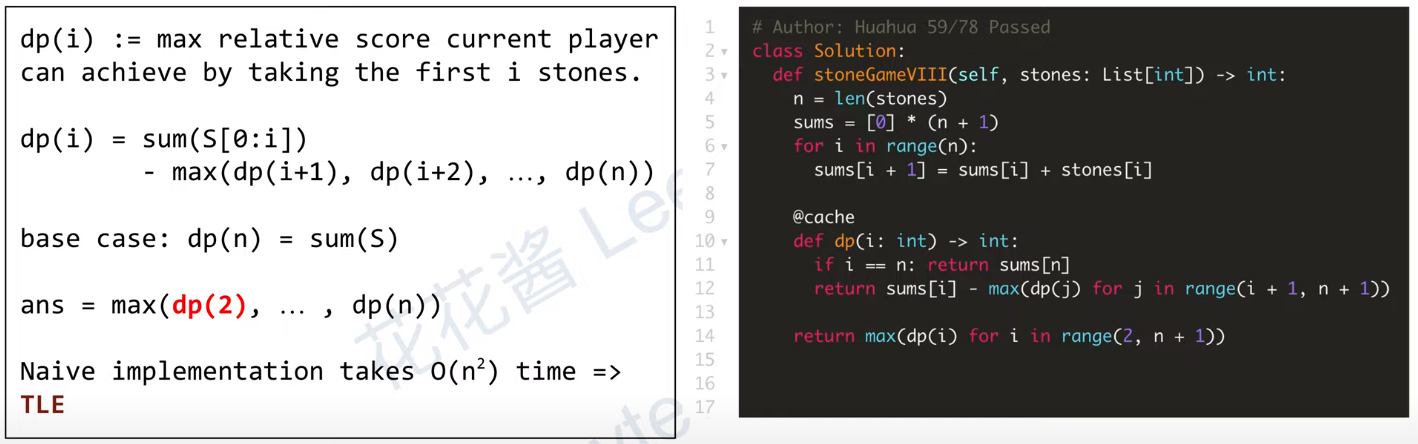
\includegraphics[width=.9\linewidth]{./pic/stone8.png}

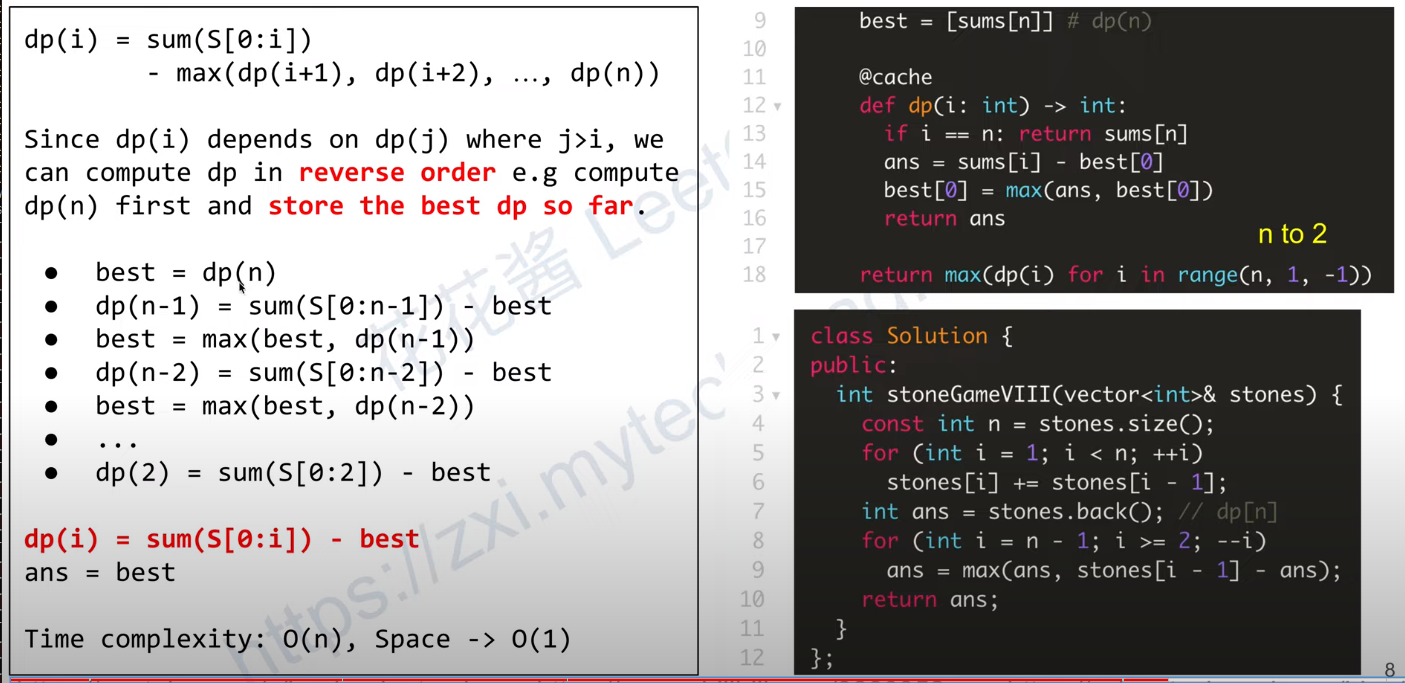
\includegraphics[width=.9\linewidth]{./pic/stone82.png}


\begin{minted}[fontsize=\scriptsize,linenos=false]{csharp}
// 使用 dp(i) 表示还剩下 [i, n) 要选择的情况下,Alice 所能得到的最大分数差。
//     对于某个玩家来说,其对应决策可以分为两种:
//     选取当前数及之前的所有数(等价于 pres[pos],其中 pos 为上个玩家选完后的下个位置),那么 dp[i] = pres[i] - dp[i+1]。
//     这是因为 bob 也会最大化发挥。
//     不选择当前数(可能选下一个,下下一个。。。 etc),那么 dp[i] = dp[i + 1]
public int stoneGameVIII(int[] stones) {
    int n = stones.length;
    int [] dp = new int [n];
    Arrays.fill(dp, Integer.MIN_VALUE);
    int [] pre = new int [n+1];
    for (int i = 1; i <= n; i++)
        pre[i] = pre[i-1] + stones[i-1];
    dp[n-1] = pre[n];
    for (int i = n-2; i >= 0; i--) 
        dp[i] = Math.max(dp[i+1], pre[i+1]-dp[i+1]);
    return dp[1];
}
\end{minted}
\begin{itemize}
\item 更精简的代码如下
\end{itemize}
\begin{minted}[fontsize=\scriptsize,linenos=false]{csharp}
public int stoneGameVIII(int[] stones) {
    int n = stones.length;
    for (int i = 1; i < n; i++) 
        stones[i] += stones[i-1]; // 原位求前缀和
    int ans = stones[n-1];
    for (int i = n-1; i >= 2; i--) 
        ans = Math.max(ans, stones[i-1] - ans); // 一遍反向遍历求最优解
    return ans;
}
\end{minted}
\end{enumerate}

\subsection{464. Can I Win 这个题:为什么顺序无关了?}
\label{sec-1-1-5}
In the "100 game" two players take turns adding, to a running total, any integer from 1 to 10. The player who first causes the running total to reach or exceed 100 wins.
What if we change the game so that players cannot re-use integers?
For example, two players might take turns drawing from a common pool of numbers from 1 to 15 without replacement until they reach a total >= 100.
Given two integers maxChoosableInteger and desiredTotal, return true if the first player to move can force a win, otherwise, return false. Assume both players play optimally.
\begin{minted}[fontsize=\scriptsize,linenos=false]{csharp}
// state是前走的人走完之后的局面,sum是当前数字总和,返回的是当前走的人是否能赢
private boolean dfs(int max, int target, int state, int val) {
    if (dp[state] != -1) return dp[state] > 0;
    if (val >= target) { // 如果对方取数的时候总和达到target了,则当前走的人输了,做记忆并返回false
        dp[state] = 0;
        return false;
    }
    for (int i = 1; i <= max; i++) {  // 枚举当前人取哪个数
        if ((state >> i-1 & 1) == 0 && !dfs(max, target, state | (1 << i-1), val + i)) {
            dp[state] = 1;
            return true;
        }
    }
    dp[state] = 0;
    return false;
}
int [] dp;
public boolean canIWin(int maxChoosableInteger, int desiredTotal) {
    if (desiredTotal <= maxChoosableInteger) return true;
    if (desiredTotal > (maxChoosableInteger + 1)*maxChoosableInteger / 2) return false;
    dp = new int[1 << maxChoosableInteger]; // 时空复杂度O ( 2 m ) O(2^m)O(2 
    Arrays.fill(dp, -1);
    return dfs(maxChoosableInteger, desiredTotal, 0, 0);
}
\end{minted}
\begin{itemize}
\item 另外这第二次又看见的解法
\end{itemize}
\begin{minted}[fontsize=\scriptsize,linenos=false]{csharp}
public boolean canIWin(int maxChoosableInteger, int desiredTotal) { // 这个师与其它类假题相比,为什么顺序无关?
    if (desiredTotal == 0) return true; // 如果1到最大能选的值所有和都不能满足目标值,那么肯定失败
    if ((maxChoosableInteger+1) * maxChoosableInteger / 2 < desiredTotal) return false;
    char [] state = new char [maxChoosableInteger];
    for (int i = 0; i < maxChoosableInteger; i++) state[i] = '0';
    return dfs(desiredTotal, state, new HashMap<>());
}
private boolean dfs(int sum, char [] st, Map<String, Boolean> map) {
    String key = new String(st);
    if (map.containsKey(key)) return map.get(key);
    for (int i = 0; i < st.length; i++) {
        if (st[i] != '0') continue;
        st[i] = '1';
        if (sum <= i+1 || !dfs(sum - (i+1), st, map)) {
            map.put(key, true);
            st[i] = '0';
            return true;
        }
        st[i] = '0';
    }
    map.put(key, false);
    return false;
}
\end{minted}
\begin{itemize}
\item // 下面这个效率更高
\end{itemize}
\begin{minted}[fontsize=\scriptsize,linenos=false]{csharp}
public boolean canIWin(int maxChoosableInteger, int desiredTotal) { 
    if (desiredTotal <= 0) return true;
    int sum = (maxChoosableInteger + 1) * maxChoosableInteger / 2;
    if (sum < desiredTotal) return false;
    boolean[] vis = new boolean[maxChoosableInteger+1];
    return helper(desiredTotal, vis);
}
Map<Integer, Boolean> map = new HashMap<>();
public boolean helper(int desiredTotal, boolean[] vis) {
    if (desiredTotal <= 0) return false;
    int symbol = format(vis);
    if (map.containsKey(symbol)) return map.get(symbol);
    for (int i = 1 ; i < vis.length ; i++) {
        if (!vis[i]) {
            vis[i] = true;
            if (!helper(desiredTotal-i, vis)) {
                vis[i] = false; // 这里不回复状态会影响其它结果
                map.put(symbol, true);
                return true;
            }
            vis[i] = false;
        }
    }
    map.put(symbol, false);
    return false;
}
public int format(boolean[] vis) {
    int symbol = 0;
    for (boolean select : vis) {
        symbol <<= 1;
        if (select) symbol |= 1;
    }
    return symbol;
}
\end{minted}

\subsection{494. Target Sum - Medium}
\label{sec-1-1-6}
You are given an integer array nums and an integer target.

You want to build an expression out of nums by adding one of the symbols '+' and '-' before each integer in nums and then concatenate all the integers.

For example, if nums = [2, 1], you can add a '+' before 2 and a '-' before 1 and concatenate them to build the expression "+2-1".
Return the number of different expressions that you can build, which evaluates to target.
\begin{itemize}
\item 该题是一道非常经典的题目,在面试中很可能会考到。该题有多种解法。
\item 第一种解法:DFS,brute force。我们对nums数组中的每个数字,都尝试在其前面添加正号和负号,最后暴力求解,统计数组中各数字组合值为target的情况。(该理解是错误的,我们可以使用带备忘录机制的自顶向下的DP方法,代码见下)
\end{itemize}
\begin{enumerate}
\item 回溯 O(2\^{}N)
\label{sec-1-1-6-1}
\begin{minted}[fontsize=\scriptsize,linenos=false]{csharp}
private int getAllSums(int [] a, int target, int idx, int sum, int cnt) { // (2^20) 可否一试呢?理论上是可以过的
    if (idx == a.length) {                                                // n < 17 比较好 这个2^N的复朵度,真要命呀。。。。。。
        if (sum == target) cnt++;
        return cnt; // 有return int代码更简洁,但是全局变量cnt效率更高
    }
    // for (int i = idx; i < a.length; i++) { // 为什么要画蝇添足,加个多余的for loop呢? 
        // getAllSums(a, target, idx+1, sum + a[idx]);
        // getAllSums(a, target, idx+1, sum - a[idx]);
    // }
    return getAllSums(a, target, idx+1, sum + a[idx], cnt)
        + getAllSums(a, target, idx+1, sum - a[idx], cnt);
}
public int findTargetSumWays(int[] a, int target) { 
    int n = a.length;
    return getAllSums(a, target, 0, 0, 0);
}
\end{minted}
\item 解题思路与分析: dfs记忆化搜索
\label{sec-1-1-6-2}
\begin{minted}[fontsize=\scriptsize,linenos=false]{csharp}
private int dfs(int [] a, int target, int idx, int sum) {
    String key = idx + "_" + sum;
    if (dp.containsKey(key)) return dp.get(key);
    if (idx == n) {
        if (sum == target) return 1;
        else return 0;
    }
    int add = dfs(a, target, idx+1, sum + a[idx]);
    int sub = dfs(a, target, idx+1, sum - a[idx]);
    dp.put(key, add+sub);
    return add + sub;
}
Map<String, Integer> dp = new HashMap<>();
int n;
public int findTargetSumWays(int[] a, int target) {
    n = a.length;
    return dfs(a, target, 0, 0);
}
\end{minted}
\begin{itemize}
\item 上面的方法比较慢,下面这个效率更好一点儿
\end{itemize}
\begin{minted}[fontsize=\scriptsize,linenos=false]{csharp}
private int dfs(int [] a, int sum, int idx) {
    if (idx == a.length) {
        if (sum == 0) return 1;
        else return 0;
    }
    Map<Integer, Integer> tmp = dp.get(idx);
    if (tmp != null) {
        if (tmp.containsKey(sum))
            return tmp.get(sum);
    } else {
        tmp = new HashMap<>();
        dp.put(idx, tmp);
    }
    int cnt = dfs(a, sum - a[idx], idx+1) + dfs(a, sum + a[idx], idx+1);
    tmp.put(sum, cnt);
    return cnt;
}
Map<Integer, Map<Integer, Integer>> dp = new HashMap<>();
public int findTargetSumWays(int[] nums, int target) {
    return dfs(nums, target, 0);
}
\end{minted}
\item DP
\label{sec-1-1-6-3}
\begin{minted}[fontsize=\scriptsize,linenos=false]{csharp}
// sum[p] + sum[n] = sum[nums];
// sum[p] - sum[n] = S;
// 2sum[p] = sum[nums] + S
// sum[p] = (sum[nums] +S) / 2
public int findTargetSumWays(int [] a, int S) {
    int sum = Arrays.stream(a).sum(), target = (sum + S) / 2; // 根据推导公式,计算出target
    if (S > 0 && sum < S || S < 0 && -sum > S) return 0; // 如果和小于S,说明无法得到解,返回false。(注意S有可能为负)
    if ((sum + S) % 2 != 0) return 0; // 如果计算出的target不是整数,返回false。
    int [] dp = new int [target + 1]; // dp[i]表示在原数组中找出一些数字,并且他们的和为下标i的可能有多少种。
    dp[0] = 1; // 初始化dp[0]为1
    for (Integer v : a) 
        // for (int i = target-v; i >= 0; i--) { // 从0循环到target - n, 注意逆序
        //     if (dp[i] > 0)        // dp[i]大于0说明,存在dp[i]种组合,其和为i的可能性
        //         dp[i+v] += dp[i]; // 既然存在和为i的可能,那么i加上当前数字的和也是存在的
        // }
        for (int i = target; i >= v; i--)  // 从0循环到target - n, 注意逆序
            dp[i] += dp[i-v];              // 两种写法都对
    return dp[target];
}
\end{minted}
\item dp todo
\label{sec-1-1-6-4}
我们使用Vi来表示数组中的前i个数所能求得的和的集合。初始化时
\begin{minted}[fontsize=\scriptsize,linenos=false]{csharp}
V0 = {0}     //表示前0个数的和为0
Vi = {V(i-1) + ai} U {V(i-1) - ai}
\end{minted}

Vn就是nums数组所有数字的组合值之和的集合

根据上面的思路,我们知道数组中数字若全为正号其和为sum,全为负号其和为-sum。若不选数组中任何一个数,则和为0。因此,我们设立一个长度为2*sum+1的数组ways,ways[i]表示我们选择前m个数,其和可能为i的情况数,m = 0,1,\ldots{}nums.length。可参考下图

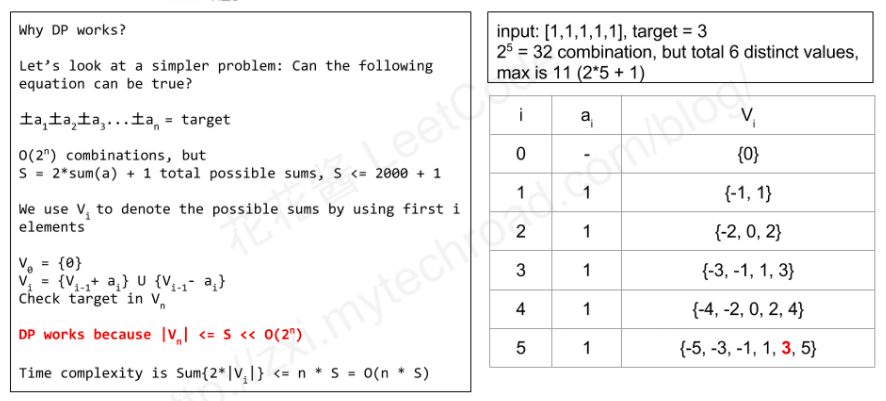
\includegraphics[width=.9\linewidth]{./pic/targetSum.png}

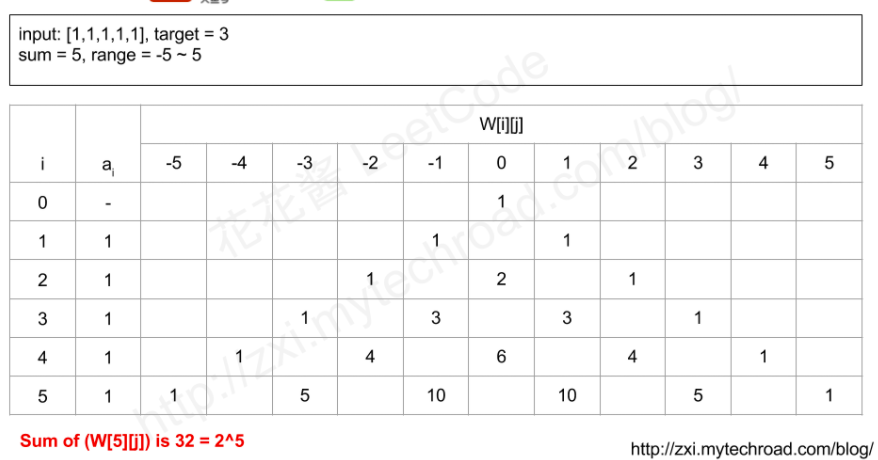
\includegraphics[width=.9\linewidth]{./pic/targetSum2.png}

\url{https://www.cnblogs.com/cnoodle/p/14869498.html}
\url{https://leetcode.com/problems/target-sum/discuss/97334/Java}-(15-ms)-C++-(3-ms)-O(ns)-iterative-DP-solution-using-subset-sum-with-explanation/239290
\url{http://www.noteanddata.com/leetcode-494-Target-Sum-java-solution-note.html}
\url{https://www.i4k.xyz/article/gqk289/54709004}
\url{https://github.com/cherryljr/LeetCode/blob/master/Target\%20Sum.java}
\end{enumerate}

\subsection{647. Palindromic Substrings - Medium}
\label{sec-1-1-7}
Given a string s, return the number of palindromic substrings in it.

A string is a palindrome when it reads the same backward as forward.

A substring is a contiguous sequence of characters within the string.
\begin{minted}[fontsize=\scriptsize,linenos=false]{csharp}
public int countSubstrings(String t) {
    int n = t.length(), ans = 0;
    char [] s = t.toCharArray();
    boolean [][] dp = new boolean [n][n];
    for (int i = n-1; i >= 0; i--) 
        for (int j = i; j < n; j++) {
            dp[i][j] = s[i] == s[j] && (j-i <= 2 || dp[i+1][j-1]);
            if (dp[i][j]) ans++;
        }
    return ans;
}
\end{minted}
\subsection{1444. Number of Ways of Cutting a Pizza - Hard}
\label{sec-1-1-8}
Given a rectangular pizza represented as a rows x cols matrix containing the following characters: 'A' (an apple) and '.' (empty cell) and given the integer k. You have to cut the pizza into k pieces using k-1 cuts. 

For each cut you choose the direction: vertical or horizontal, then you choose a cut position at the cell boundary and cut the pizza into two pieces. If you cut the pizza vertically, give the left part of the pizza to a person. If you cut the pizza horizontally, give the upper part of the pizza to a person. Give the last piece of pizza to the last person.

Return the number of ways of cutting the pizza such that each piece contains at least one apple. Since the answer can be a huge number, return this modulo 10\^{}9 + 7.
\begin{enumerate}
\item 解题思路与分析: 自底向上
\label{sec-1-1-8-1}

常规的矩阵DP做法,这里还需要通过前缀和的思想来快速获取指定范围矩阵的苹果数量。

首先是建立状态表示数组,通过一个三维数组,分别代表矩阵左上角顶点xy坐标和需要分配的人数,数组值表示分该状态下的配方案数;

然后是进行状态转移,从右下角开始枚举所有以该点为状态中左上角的状态,再从低到高枚举需要分配的人数,接着进行切的操作,可以横着切和竖着切,分别枚举所有可能的切除的长度,当前状态的方案数需要从切除后剩下的矩阵状态中进行转移累加。

最后返回以原矩阵左上角为顶点的,分配人数为k的方案数即可。

这里为什么需要将状态表示中的xy设定为矩阵的左上角,还有为什么苹果数的前缀和也是求的右下角的前缀和呢?

因为题意中的切除操作后,要将上半部分或者左半部分给分掉,所以只有右下部分是剩余状态的,我们需要从切除之前的状态获取剩余状态。

\begin{minted}[fontsize=\scriptsize,linenos=false]{csharp}
public int ways(String[] pizza, int p) {
    int mod = (int)1e9 + 7;
    int m = pizza.length, n = pizza[0].length();
    int [][] cnt = new int [m+1][n+1]; // 苹果数的前缀和,用于快速获得在指定矩阵范围内的苹果数量,两个维度也分别是左上角的x、y
    for (int i = m-1; i >= 0; i--) 
        for (int j = n-1; j >= 0; j--) 
            cnt[i][j] = cnt[i+1][j] + cnt[i][j+1] - cnt[i+1][j+1] + (pizza[i].charAt(j) == 'A' ? 1 : 0);
    int [][][] dp = new int [m+1][n+1][p+1]; // 状态数组,三个维度分别表示以x、y为左上角的矩阵中,分给k个人,元素值表示方案数
    for (int i = m-1; i >= 0; i--)       // 遍历矩阵,获取指定左上角矩阵中范围内的苹果数量
        for (int j = n-1; j >= 0; j--) { // 从右下角开始,向左上角开始枚举所有状态
            if (cnt[i][j] > 0) dp[i][j][1] = 1; // 如果这个范围矩阵内存在苹果,那么这个矩阵肯定可以分给1个人,且方案数为1
            for (int k = 2; k <= p; k++) {      // 枚举所有人数状态下的方案,前面已经判断了人数为1的状态,所以这里只需要从2开始枚举
                for (int x = m-1-i; x >= 0; x--)     // 横着切,枚举所有切法
                    if (cnt[i][j] - cnt[i+x][j] > 0) // 如果当前切掉的矩阵内存在苹果,则可以进行状态转移
                        dp[i][j][k] = (dp[i][j][k] + dp[i+x][j][k-1]) % mod;
                for (int y = n-1-j; y >= 0; y--)     // 竖着切
                    if (cnt[i][j] - cnt[i][j+y] > 0)
                        dp[i][j][k] = (dp[i][j][k] + dp[i][j+y][k-1]) % mod;
            }
        }
    return (int)dp[0][0][p];
}
\end{minted}
\item 解题思路与分析: 自顶向下
\label{sec-1-1-8-2}

先用dp方法求出以(i,j)位置为右下角,左上角为(0,0)的区域的苹果数量

建立3维数组,dp[i][j][k]表示切完k次后,剩余蛋糕左上角 在i, j位置时的方案数

初始化,dp\footnote{DEFINITION NOT FOUND.}\textsuperscript{,}\,\footnotemark[1]{}\textsuperscript{,}\,\footnotemark[1]{} = 1

样本维度为切的次数 k

状态维度,这次切之前的状态(蛋糕左上角位置 i, j)

状态转移,这次切完后蛋糕左上角位置(横向切,ni,j;竖向切,i, nj,切的次数 +1)

转移条件:切出去的蛋糕当中有苹果(用上面求得的苹果数量,dp公式求得)

最后求结果总和:最后的一块蛋糕中有苹果,sum += dp[i][j][k-1]
\begin{minted}[fontsize=\scriptsize,linenos=false]{csharp}
public int ways(String[] pizza, int p) { // 自顶向下: 与自底向上相比
    int mod = (int)1e9 + 7;
    int m = pizza.length, n = pizza[0].length();
    int [][] cnt = new int [m+1][n+1];  // 苹果数的前缀和,用于快速获得在指定矩阵范围内的苹果数量,两个维度也分别是左上角的x、y
    for (int i = 1; i <= m; i++) 
        for (int j = 1; j <= n; j++) 
            cnt[i][j] = cnt[i-1][j] + cnt[i][j-1] - cnt[i-1][j-1] + (pizza[i-1].charAt(j-1) == 'A' ? 1 : 0);
    int [][][] dp = new int [m+1][n+1][p]; // dp[i][j][k]表示切完k次后,剩余蛋糕左上角 在i,j位置时的方案数
    dp[1][1][0] = 1; // 初始值是为了程序的运行,
    for (int k = 1; k < p; k++) 
        for (int i = 1; i <= m; i++) 
            for (int j = 1; j <= n; j++) {
                System.out.println("(dp[i][j][k-1] == 0) : " + (dp[i][j][k-1] == 0) );
                if (dp[i][j][k-1] == 0) continue; // 上一次cut完后,剩余蛋糕左上角在i,j
                for (int x = i+1; x <= m; x++)   // 横向切,切完后的剩余左上角为 x, j
                    if (cnt[x-1][n] - cnt[i-1][n] - cnt[x-1][j-1] + cnt[i-1][j-1] > 0)
                        dp[x][j][k] = (dp[x][j][k] + dp[i][j][k-1]) % mod;
                for (int y = j+1; y <= n; y++)  // 竖向切
                    if (cnt[m][y-1] - cnt[m][j-1] - cnt[i-1][y-1] + cnt[i-1][j-1] > 0)
                        dp[i][y][k] = (dp[i][y][k] + dp[i][j][k-1]) % mod;
            }
    long ans = 0;
    for (int i = 1; i <= m; i++) 
        for (int j = 1; j <= n; j++) 
            if (cnt[m][n] - cnt[i-1][n] - cnt[m][j-1] + cnt[i-1][j-1] > 0) // 先前并没有确认切的结果有效,即最后剩下的那块是否有苹果
                ans = (ans + dp[i][j][p-1]) % mod;                         // 统计结果的时候,要先确保有效
    return (int)ans;
}
\end{minted}
\end{enumerate}


\section{字符串、数组等双序列}
\label{sec-1-2}

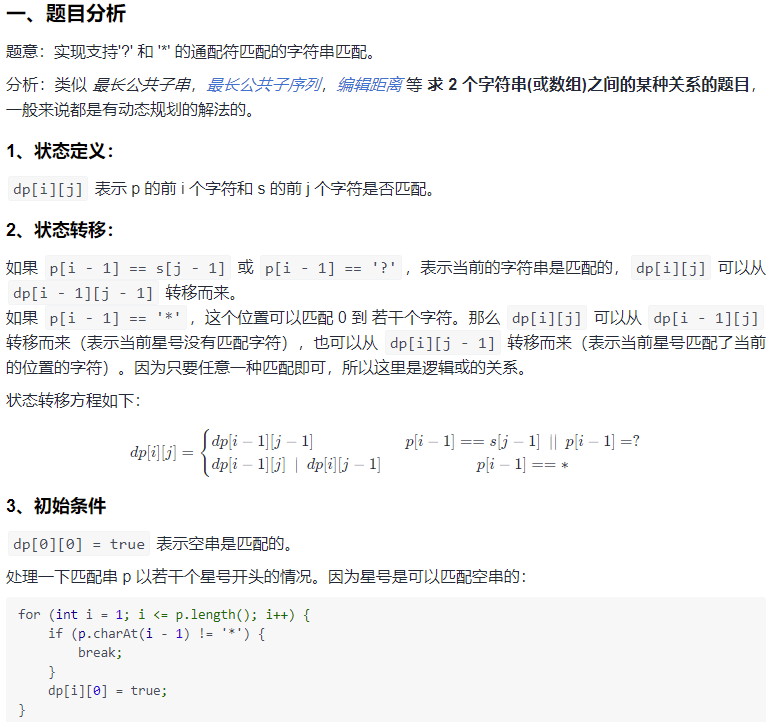
\includegraphics[width=.9\linewidth]{./pic/doubSeq.png}

\subsection{题目拓展}
\label{sec-1-2-1}
\begin{enumerate}
\item 718. 最长重复子数组 (类似题目,只是由字符串变为数组)
\label{sec-1-2-1-1}
\item 72. 编辑距离
\label{sec-1-2-1-2}
\item 1143. 最长公共子序列
\label{sec-1-2-1-3}
\item 10. 正则表达式匹配
\label{sec-1-2-1-4}
\item 583. 两个字符串的删除操作
\label{sec-1-2-1-5}
\item 727. 最小窗口子序列
\label{sec-1-2-1-6}

你会发现这些都是 求 2 个字符串(或数组)之间的某种关系的题目
\end{enumerate}
\subsection{10. Regular Expression Matching - Hard}
\label{sec-1-2-2}
Given an input string s and a pattern p, implement regular expression matching with support for '.' and '*' where:

'.' Matches any single character.​​​​
'*' Matches zero or more of the preceding element.
The matching should cover the entire input string (not partial).
\begin{enumerate}
\item 解题思路与分析
\label{sec-1-2-2-1}

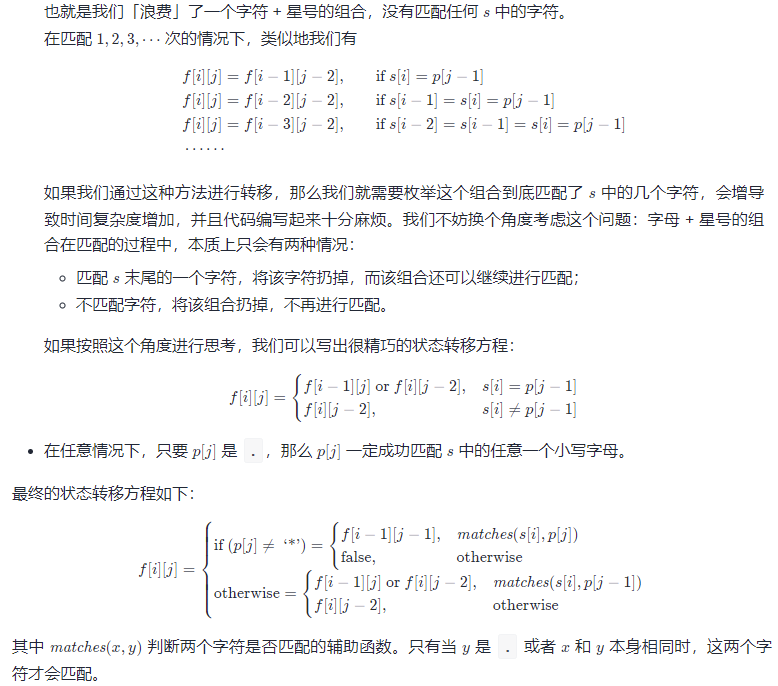
\includegraphics[width=.9\linewidth]{./pic/regMatch.png}

\begin{minted}[fontsize=\scriptsize,linenos=false]{csharp}
public boolean isMatch(String s, String p) {
    int m = s.length();
    int n = p.length();
    boolean[][] f = new boolean[m + 1][n + 1];
    f[0][0] = true;
    for (int i = 0; i <= m; ++i) 
        for (int j = 1; j <= n; ++j) 
            if (p.charAt(j - 1) == '*') {
                f[i][j] = f[i][j - 2];
                if (matches(s, p, i, j - 1)) 
                    f[i][j] = f[i][j] || f[i - 1][j];
            } else {
                if (matches(s, p, i, j)) 
                    f[i][j] = f[i - 1][j - 1];
            }
    return f[m][n];
}
public boolean matches(String s, String p, int i, int j) {
    if (i == 0) return false;
    if (p.charAt(j - 1) == '.') return true;
    return s.charAt(i - 1) == p.charAt(j - 1);
}
\end{minted}
\end{enumerate}
\subsection{115. Distinct Subsequences - Hard}
\label{sec-1-2-3}
Given two strings s and t, return the number of distinct subsequences of s which equals t.

A string's subsequence is a new string formed from the original string by deleting some (can be none) of the characters without disturbing the remaining characters' relative positions. (i.e., "ACE" is a subsequence of "ABCDE" while "AEC" is not).

It is guaranteed the answer fits on a 32-bit signed integer.
\begin{enumerate}
\item 解题思路与分析
\label{sec-1-2-3-1}
这道题不是求两个字符串是匹配,而是判断S有多少种方式可以得到T。但其实还是动态规划,我们一个定义二维数组dp,dp[i][j]为字符串s(0,i)变换到t(0,j)的变换方法的个数。

如果S[i]==T[j],那么dp[i][j] = dp[i-1][j-1] + dp[i-1][j]

意思是:如果当前S[i]==T[j],那么当前这个字符即可以保留也可以抛弃,所以变换方法等于保留这个字符的变换方法加上不用这个字符的变换方法, 

dp[i-1][j-1]为保留这个字符时的变换方法个数,dp[i-1][j]表示抛弃这个字符时的变换方法个数。

如果S[i]!=T[i],那么dp[i][j] = dp[i-1][j],意思是如果当前字符不等,那么就只能抛弃当前这个字符。

\begin{minted}[fontsize=\scriptsize,linenos=false]{csharp}
public int numDistinct(String ss, String tt) {
    int m = ss.length(), n = tt.length();
    char [] s = ("#"+ss).toCharArray();
    char [] t = ("#"+tt).toCharArray();
    int [][] dp = new int [m+1][n+1];
    dp[0][0] = 1;
    for (int j = 1; j <= n; j++) // 注意这两行初始状态的设置
        dp[0][j] = 0;
    for (int i = 1; i <= m; i++) 
        dp[i][0] = 1;
    for (int i = 1; i <= m; i++) 
        for (int j = 1; j <= n; j++) 
            if (s[i] == t[j])
                dp[i][j] = dp[i-1][j-1] + dp[i-1][j];
            else dp[i][j] = dp[i-1][j];
    return dp[m][n];
}
\end{minted}
\end{enumerate}

\subsection{将一个数组分为两个部分,分别求和S1与S2,使得|S1-S2|最小}
\label{sec-1-2-4}

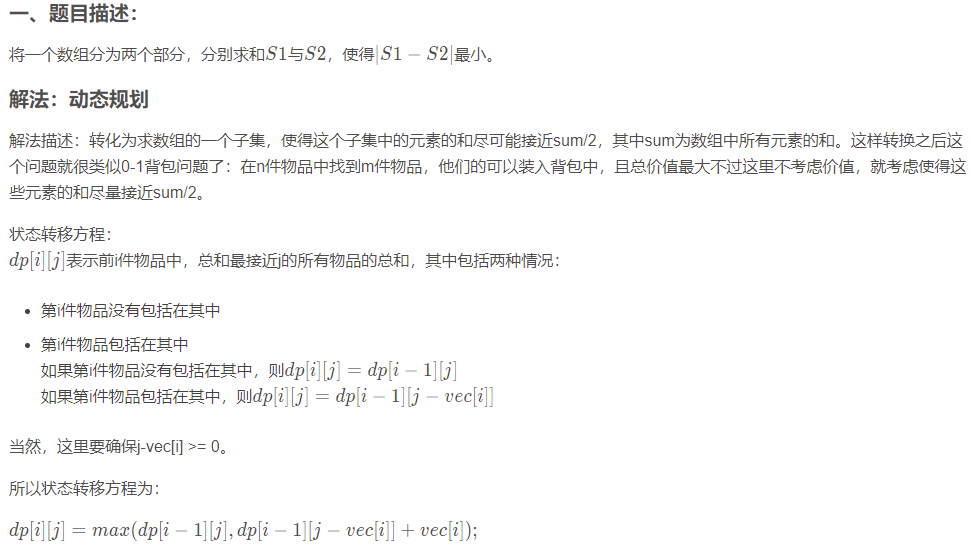
\includegraphics[width=.9\linewidth]{./pic/dpArray.png}

\begin{minted}[fontsize=\scriptsize,linenos=false]{csharp}
public static int getMaxDiff(int[] array) {
    int sum = Arrays.stream(array).sum();
    int length = array.length;
    int [][] f = new int[length+1][sum/2+1];
    for (int i = 0; i < length; i++) 
        for (int j = 1; j <  = sum/2; j++) {
            f[i+1][j]  =  f[i][j];
            if (array[i] <= j && f[i][j-array[i]] + array[i] > f[i][j]) 
                f[i+1][j] = f[i][j-array[i]] + array[i];
        }
    return sum-2*f[length][sum/2];
}
\end{minted}
\subsection{给定一个序列,不保证有序,求这个序列的最长等差序列的长度。}
\label{sec-1-2-5}

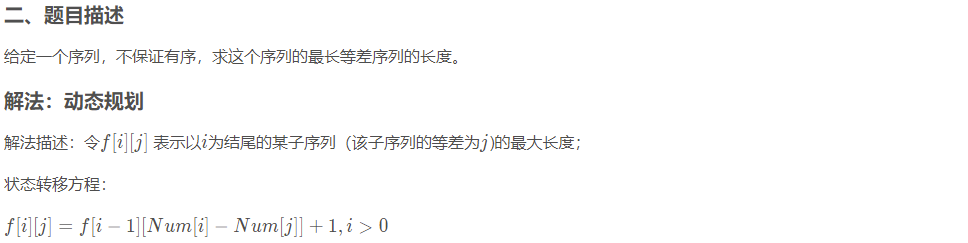
\includegraphics[width=.9\linewidth]{./pic/dpArray2.png}

\begin{minted}[fontsize=\scriptsize,linenos=false]{csharp}
private static int lengthOfLongest(int[] set){
    Arrays.sort(set);
    int n = set.length;
    if (n <= 2) return n;
    int llap = 2;
    int[][] dp = new int[n][n];
    for (int i=0; i<n; i++) dp[i][n-1] = 2;
    for (int j=n-2; j>=1; j--) {
        int i=j-1, k=j+1;
        while (i>=0 && k<=n-1) {
            if (set[i] + set[k] < 2 * set[j])
                k++;
            else if (set[i] + set[k] > 2 * set[j]) {
                dp[i][j] = 2;
                i--;
            } else {
                dp[i][j] = dp[j][k] + 1;
                llap = Math.max(llap, dp[i][j]);
                i--;
                k++;
            }
        }
        while (i >= 0) {
            dp[i][j] = 2;
            i--;
        }
    }
    return llap;
}
\end{minted}
\subsection{求一个序列的最长子序列,使得最多修改一个数字使得这个子序列的为严格递增序列}
\label{sec-1-2-6}

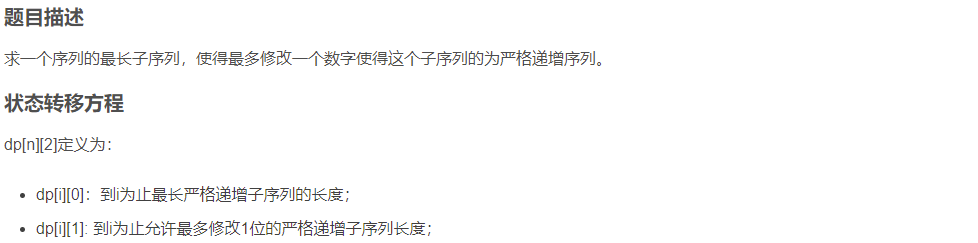
\includegraphics[width=.9\linewidth]{./pic/dpArray3.png}
\begin{minted}[fontsize=\scriptsize,linenos=false]{csharp}
private static int getMaxLength(int[] arr){
    if (arr.length <= 2) return arr.length;
    int[][] dp = new int[arr.length][2];
    dp[0][0] = 1;
    dp[0][1] = 1;
    for (int i = 1; i < arr.length; i++) {
        dp[i][0] = dp[i-1][0]+1;
        if (arr[i] <= arr[i-1])
            dp[i][0]--;
        if (dp[i-1][0] == dp[i-1][1] && arr[i] <= arr[i-1]) {// 说明前面还没有改的
            dp[i][1] = dp[i][0] + 1;
            arr[i] = arr[i-1]+1;
        } else {//说明前面已经改动或者arr[i] <= arr[i-1]
            if (arr[i] > arr[i-1]) {
                //判断前面是否已经改动
                dp[i][1] = dp[i-1][1]+1;
                if (dp[i-1][0] != dp[i-1][1]) 
                    dp[i][1]--;
            } else
                dp[i][1] = dp[i-1][1];
        }
    }
    return dp[arr.length-1][1];
}
\end{minted}

\subsection{801. Minimum Swaps To Make Sequences Increasing - Hard}
\label{sec-1-2-7}
You are given two integer arrays of the same length nums1 and nums2. In one operation, you are allowed to swap nums1[i] with nums2[i].

For example, if nums1 = [1,2,3,8], and nums2 = [5,6,7,4], you can swap the element at i = 3 to obtain nums1 = [1,2,3,4] and nums2 = [5,6,7,8].
Return the minimum number of needed operations to make nums1 and nums2 strictly increasing. The test cases are generated so that the given input always makes it possible.

An array arr is strictly increasing if and only if arr\footnotemark[1]{} < arr\footnote{DEFINITION NOT FOUND.} < arr\footnote{DEFINITION NOT FOUND.} < \ldots{} < arr[arr.length - 1].
\begin{enumerate}
\item 解题思路与分析
\label{sec-1-2-7-1}
\begin{minted}[fontsize=\scriptsize,linenos=false]{csharp}
// 设 dp[0][i] 表示不交换 A[i] 和 B[i] 在下标 i 的交换次数
// 设 dp[1][i] 表示交换 A[i] 和 B[i] 在下标 i 的交换次数
// 可以看到交换与否只取决与前一个状态, 可以将空间复杂度压缩到 O(1)
//     时间复杂度为 O(n), 空间复杂度为 O(1)
public int minSwap(int[] a, int[] b) {
    int n = a.length;
    int [][] dp = new int [n][2]; // 0: 不换, 1: 换
    for (int i = 0; i < n; i++) 
        Arrays.fill(dp[i], Integer.MAX_VALUE);
    dp[0][0] = 0;
    dp[0][1] = 1;
    for (int i = 1; i < n; i++) {
        if (a[i] > a[i-1] && b[i] > b[i-1]) {
            dp[i][0] = Math.min(dp[i][0], dp[i-1][0]);     // 不换,取一个较小值
            dp[i][1] = Math.min(dp[i][1], dp[i-1][1] + 1); // 换就两个都换
        }
        if (a[i] > b[i-1] && b[i] > a[i-1]) {
            dp[i][0] = Math.min(dp[i][0], dp[i-1][1]); 
            dp[i][1] = Math.min(dp[i][1], dp[i-1][0] + 1);
        }
    }
    return Math.min(dp[n-1][0], dp[n-1][1]);
}
\end{minted}
\end{enumerate}

\subsection{1639. Number of Ways to Form a Target String Given a Dictionary - Hard}
\label{sec-1-2-8}
You are given a list of strings of the same length words and a string target.

Your task is to form target using the given words under the following rules:

target should be formed from left to right.
To form the ith character (0-indexed) of target, you can choose the kth character of the jth string in words if target[i] = words[j][k].
Once you use the kth character of the jth string of words, you can no longer use the xth character of any string in words where x <= k. In other words, all characters to the left of or at index k become unusuable for every string.
Repeat the process until you form the string target.
Notice that you can use multiple characters from the same string in words provided the conditions above are met.

Return the number of ways to form target from words. Since the answer may be too large, return it modulo 109 + 7.
\begin{enumerate}
\item 解题思路与分析: dp
\label{sec-1-2-8-1}
\begin{minted}[fontsize=\scriptsize,linenos=false]{csharp}
   思路:
   dp[i][j]  表示:words字符串列表的前 j 列来构造目标字符串target的前 i 个字符;
   cnt[i][j] 表示:words字符串列表的第 i 列 一共有多少 字符 j ;
   那dp公式就很好推出来了:
   1.第i个字符不使用第j列时,即通过前 j - 1 列得到
     dp[i][j] = dp[i][j-1];
   2.第i个字符使用第j列时
   *   dp[i][j] = dp[i-1][j-1] * cnt[j][第i个字符];
   ==>>dp[i][j] = dp[i][j-1] + dp[i-1][j-1] * cnt[j][第i个字符]
\end{minted}
\begin{minted}[fontsize=\scriptsize,linenos=false]{csharp}
static final int mod = (int)1e9 + 7;
public int numWays(String[] words, String target) {
    int m = target.length(), n = words[0].length();
    char [] s = target.toCharArray();
    int [][] cnt = new int [n][26];
    for (String w : words) 
        for (int j = 0; j < n; j++) 
            cnt[j][w.charAt(j)-'a']++;
    // long [][] dp = new long [m][n];
    // dp[0][0] = cnt[0][s[0]-'a'];
    // for (int i = 1; i < n; i++) // 初始化: 由前i列来构成target第一个字符的方案数
    //     dp[0][i] = (dp[0][i] + dp[0][i-1] + cnt[i][s[0]-'a']) % mod;
    // for (int i = 1; i < m; i++) 
    //     for (int j = i; j < n; j++) 
    //         dp[i][j] = (dp[i][j-1] + dp[i-1][j-1] * cnt[j][s[i]-'a']) % mod;
    // return (int)dp[m-1][n-1];
    long [][] dp = new long [m+1][n+1];
    Arrays.fill(dp[0], 1l);
    // dp[0] = LongStream.range(0, n+1).map(e->1).toArray(); // 上下两行,效果差不多,filling first row of array with 1
    for (int i = 1; i <= m; i++)
        for (int j = i; j <= n + i - m; j++) 
            dp[i][j] = (dp[i][j-1] + dp[i-1][j-1] * cnt[j-1][s[i-1]-'a'] % mod) % mod;
    return (int)dp[m][n];
}
\end{minted}
\begin{itemize}
\item dp降维,压缩空间
\end{itemize}
\begin{minted}[fontsize=\scriptsize,linenos=false]{csharp}
static final int mod = (int)1e9 + 7;
public int numWays(String[] words, String target) { // dp降维,压缩空间,但二维dp仍然是思路最为清晰好理解的
    int m = target.length(), n = words[0].length();
    char [] s = target.toCharArray();
    long [] dp = new long [m];
    for (int i = 0; i < n; i++) {  // 遍历字符数组的各列
        int [] cnt = new int [26]; // 当前-列-所有字符的出现次数
        for (String w : words) 
            cnt[w.charAt(i)-'a']++;
        for (int j = Math.min(i, m-1); j >= 0; j--) // 记住: 降维就容易产生赃数据,需要倒序遍历
            dp[j] = (dp[j] + (j > 0 ? dp[j-1] : 1) * cnt[s[j]-'a']) % mod;
    }
    return (int)dp[m-1];
}
\end{minted}
\end{enumerate}

\section{区间型DP}
\label{sec-1-3}
\begin{itemize}
\item \url{https://leetcode-cn.com/problems/minimum-cost-to-merge-stones/solution/yi-dong-you-yi-dao-nan-yi-bu-bu-shuo-ming-si-lu-he/}
\end{itemize}

区间dp问题,旨在通过动态规划去求一个区间的最优解,通过将大区间划分为很多个小区间,再由小区间的解来组合出大区间的解,这体现了分治的思想。

\begin{itemize}
\item 区间动态规划三部曲
\begin{itemize}
\item 定义状态:dp[i, j]为区间[i, j]的最优解
\item 定义状态转移方程:最常见的写法为:dp[i,j] = max/min\{dp[i,j], dp[i, k] + dp[k+1, j] + cost\}。选取[i, j]之间的一个分界点k,分别计算[i, k]和[k+1, j]的最优解,从而组合出[i, j]的最优解。
\item 初始化:dp[i][i] = 常数。区间长度为1时的最优解应当是已知的。
\end{itemize}
\end{itemize}

假设要求的区间最优解为dp[1, n],区间dp问题有两种编码方法:

\begin{itemize}
\item 第一种:
\end{itemize}
\begin{minted}[fontsize=\scriptsize,linenos=false]{csharp}
for (int i = n; i >= 1; --i) 
    for (int j = i + 1; j <= n; ++j) 
        for (int k = i; k < j; ++k) 
            dp[i,j] = max/min(dp[i,j], dp[i,k] + dp[k+1, j] + cost)
\end{minted}

这种写法就是常规的dp写法,枚举i为子区间左边界,枚举j为子区间有边界,枚举k为分界点。要注意由于要求的是dp[1,n],所以i必须从大往小遍历,j必须从小往大遍历。这样在状态转移方程中利用的就是已求解的dp状态。
\begin{itemize}
\item 第二种:
\end{itemize}
\begin{minted}[fontsize=\scriptsize,linenos=false]{csharp}
for (int len = 2; len <= n; ++len) 
    for (int i = 1; i + len - 1  <= n; ++i) {
        int j = i + len - 1;
        for (int k = i; k < j; ++k) 
            dp[i,j] = max/min(dp[i,j], dp[i,k] + dp[k+1, j] + cost;
    }
\end{minted}

这种写法最常见,枚举len为区间长度,枚举i为区间左端点,由此可以计算出区间右端点j,枚举k为分界点。区间长度从2到n,跟上一种写法相同。这种写法的正确性可能不如上一种那么直观,它从小到大枚举出所有区间,在求解大区间时,状态转移方程中利用的状态都是小区间的状态,必定在它之前被求解,所以也是正确的。

\subsection{1039. Minimum Score Triangulation of Polygon - Medium}
\label{sec-1-3-1}
You have a convex n-sided polygon where each vertex has an integer value. You are given an integer array values where values[i] is the value of the ith vertex (i.e., clockwise order).

You will triangulate the polygon into n - 2 triangles. For each triangle, the value of that triangle is the product of the values of its vertices, and the total score of the triangulation is the sum of these values over all n - 2 triangles in the triangulation.

Return the smallest possible total score that you can achieve with some triangulation of the polygon.

\begin{minted}[fontsize=\scriptsize,linenos=false]{csharp}
// 动态规划,递归可以使逻辑简单(本质还是动态规划)将多边形起始位置设为start,end, 用一个数组dp来记录任意起始位置的score
// 为了计算dp[start][end], 我们用一个index k在start到end之间遍历
// dp[start][end] = min(dp[start][k] + dp[k][end] + A[start]* A[k] * A[end])结果为dp[0][n - 1]注意:相邻的dp[i][i + 1] = 0, 因为两条边无法组成三角形
private int dfs(int [] a, int i, int j) {
    if (j - i < 2) return 0; // 最开始终止条件没有写对
    if (dp[i][j] > 0) return dp[i][j];
    int ans = Integer.MAX_VALUE;
    for (int k = i+1; k < j; k++) 
        ans = Math.min(ans, a[i]*a[k]*a[j] + dfs(a, i, k) + dfs(a, k, j));
    return dp[i][j] = ans;
}
int [][] dp;
int n;
public int minScoreTriangulation(int[] a) {
    n = a.length;
    dp = new int [n][n];
    return dfs(a, 0, n-1);
}
\end{minted}

\subsection{2019. The Score of Students Solving Math Expression - Hard 有人说这是区间dp,无感}
\label{sec-1-3-2}
You are given a string s that contains digits 0-9, addition symbols '+', and multiplication symbols '*' only, representing a valid math expression of single digit numbers (e.g., 3+5*2). This expression was given to n elementary school students. The students were instructed to get the answer of the expression by following this order of operations:

Compute multiplication, reading from left to right; Then,
Compute addition, reading from left to right.
You are given an integer array answers of length n, which are the submitted answers of the students in no particular order. You are asked to grade the answers, by following these rules:

If an answer equals the correct answer of the expression, this student will be rewarded 5 points;
Otherwise, if the answer could be interpreted as if the student applied the operators in the wrong order but had correct arithmetic, this student will be rewarded 2 points;
Otherwise, this student will be rewarded 0 points.
Return the sum of the points of the students.
\begin{enumerate}
\item 解题思路与分析
\label{sec-1-3-2-1}
\begin{itemize}
\item 思路是记忆化搜索。先求一下正确答案,然后开始算所有可能得到的错误答案。枚举运算符,然后递归求解两边可能的答案,汇总成当前表达式可能得到的答案。用记忆化的方式避免重复计算。
\item 时间复杂度O(l\_s\^{}3+l\_A)),空间O(l\_s\^{}2)。注意有1000这个限制,上面所说的复杂度的常数是1000\^{}2,是很大的
\end{itemize}

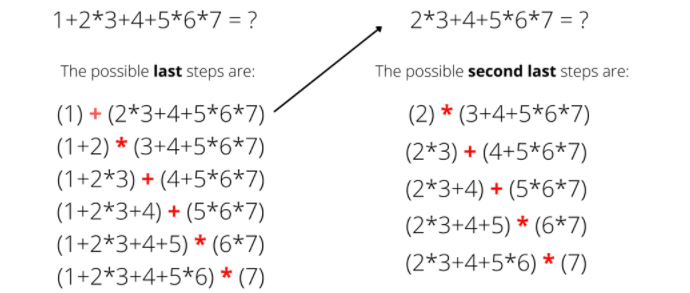
\includegraphics[width=.9\linewidth]{./pic/score.png}

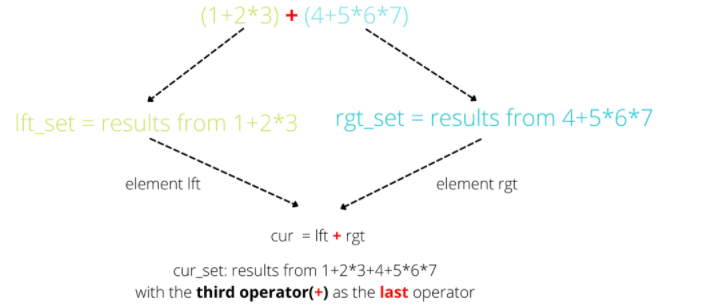
\includegraphics[width=.9\linewidth]{./pic/score2.png}

\begin{minted}[fontsize=\scriptsize,linenos=false]{csharp}
private int compute(String t) {
    ArrayDeque<Integer> st = new ArrayDeque<>();
    char [] s = t.toCharArray();
    for (int i = 0; i < s.length; i++) {
        char c = s[i];
        if (Character.isDigit(c)) 
            if (i > 0 && s[i-1] == '*') 
                st.push(st.pop() * (c-'0'));
            else st.push(c-'0');
    }
    int ans = 0;
    while (!st.isEmpty()) 
        ans += st.pop();
    return ans;
}
Set<Integer> dfs(String t, int l, int r, Set<Integer> [][] f) {
    if (f[l][r] != null) return f[l][r]; // 有记忆则调取记忆
    char [] s = t.toCharArray();
    int n = t.length(), v = 0;
    f[l][r] = new HashSet<>();
    if (l == r) {
        f[l][r].add(s[l] - '0');
        return f[l][r];
    }
    for (int i = l+1; i < r; i++) 
        if (!Character.isDigit(s[i])) { // 递归求解左右两边可能算出的答案
            Set<Integer> left = dfs(t, l, i-1, f);
            Set<Integer> right = dfs(t, i+1, r, f);
            for (Integer va : left) 
                for (Integer vb : right) {
                    if (s[i] == '*') v = va * vb;
                    else v = va + vb;
                    if (v >= 0 && v <= 1000) f[l][r].add(v);
                }
        }
    return f[l][r];
}
public int scoreOfStudents(String s, int [] num) { 
    int m = num.length, res = compute(s), n = s.length(), ans = 0;
    Set<Integer> [][] f = new HashSet[n][n]; // 第一次见,学习一下
    dfs(s, 0, n-1, f);
    Set<Integer> can = f[0][n-1];        // candidates: of wrong answers
    for (Integer v : num) 
        if (v == res) ans += 5;
        else if (can.contains(v)) ans += 2;
    return ans;
}
\end{minted}
\end{enumerate}

\subsection{312. Burst Balloons 区间型动态规划的典型代表}
\label{sec-1-3-3}
You are given n balloons, indexed from 0 to n - 1. Each balloon is painted with a number on it represented by an array nums. You are asked to burst all the balloons.
If you burst the ith balloon, you will get nums[i - 1] * nums[i] * nums[i + 1] coins. If i - 1 or i + 1 goes out of bounds of the array, then treat it as if there is a balloon with a 1 painted on it.
Return the maximum coins you can collect by bursting the balloons wisely.
\begin{minted}[fontsize=\scriptsize,linenos=false]{csharp}
public int maxCoins(int[] nums) {
    int n = nums.length;
    int [][]  dp = new int [n+2][n+2];
    int [] arr = new int [n+2];
    System.arraycopy(nums, 0, arr, 1, n);
    arr[0] = arr[n+1] = 1;  // [0, n+1] ==> [1, n]
    int j = 0;
    for (int len = 1; len <= n; len++) { // [1, n]
        for (int i = 1; i+len-1 <= n; i++) { // [1, n]
            j = i + len - 1;
            for (int k = i; k <= j; k++) 
                dp[i][j] = Math.max(dp[i][j], dp[i][k-1] + dp[k+1][j] + arr[i-1]*arr[k]*arr[j+1]);
        }
    }
    return dp[1][n];
}
// 0    0    0    0    0    0
// 0    3    30   159  167  0
// 0    0    15   135  159  0
// 0    0    0    40   48   0
// 0    0    0    0    40   0
// 0    0    0    0    0    0
private int memorizedSearch(int [] arr, int x, int y) {
    if (dp[x][y] > 0) return dp[x][y];
    // if (x == y) return dp[x][y] = arr[x]; // 没有这些个边际条件
    // if (x == y-1) 
    //     return dp[x][y] = arr[x] * arr[y] + Math.max(arr[x], arr[y]);
    int max = 0;
    for (int i = x; i <= y; i++) {
        max = Math.max(max, memorizedSearch(arr, x, i-1) + memorizedSearch(arr, i+1, y) + arr[x-1]*arr[i]*arr[y+1]);
    }
    return dp[x][y] = max;
}
int [][] dp;
int n;
public int maxCoins(int[] nums) {
    int n = nums.length + 2;
    dp = new int [n][n];
    int [] arr = new int [n];
    System.arraycopy(nums, 0, arr, 1, n-2);
    arr[0] = arr[n-1] = 1;
    return memorizedSearch(arr, 1, n-2);
}
\end{minted}

\subsection{1000. Minimum Cost to Merge Stones - Hard}
\label{sec-1-3-4}
There are n piles of stones arranged in a row. The ith pile has stones[i] stones.
A move consists of merging exactly k consecutive piles into one pile, and the cost of this move is equal to the total number of stones in these k piles.
Return the minimum cost to merge all piles of stones into one pile. If it is impossible, return -1.
\begin{enumerate}
\item 解题思路与分析
\label{sec-1-3-4-1}

看到了论坛上有人定义了三维的 dp 数组,把每次合并的堆数K也当作一维放入到 dp 数组中了,其实博主觉得不是很有必要,因为像这种必须要对 dp 数组进行升维操作的是当题目中有隐藏信息 Hidden Information,而当前定义的 dp 数组无法重现子问题,即无法找到状态转移方程的时候必须要做的,最典型的例子就是之前那道 Remove Boxes,那道题自区间的 dp 值非常依赖于区间左边相同的数字的个数,而这道题每次合并的堆数K并不是很依赖其他小于K的合并的堆数,所以博主感觉没有必要加。

\begin{minted}[fontsize=\scriptsize,linenos=false]{csharp}
public int mergeStones(int[] stones, int k) {
    int n = stones.length;
    if ((n-1) % (k-1) != 0) return -1;
    int [][] dp = new int[n][n];
    int [] pre = new int[n+1];
    for (int i = 1; i <= n; i++) 
        pre[i] = pre[i-1] + stones[i-1];
    int j = 0;
    for (int len = k; len <= n; len++) {
        for (int i = 0; i+len-1 < n; i++) {
            j = i + len -1;
            dp[i][j] = Integer.MAX_VALUE; // have to initialize it here !!!
            for (int x = i; x < j; x += k-1) 
                dp[i][j] = Math.min(dp[i][j], dp[i][x] + dp[x+1][j]);
            if ((j - i) % (k - 1) == 0) // 如果总长度满足合并只剩一个数的条件,则可以再合并一次
                dp[i][j] += pre[j+1] - pre[i];
        }
    }
    return dp[0][n-1];
}
\end{minted}
\item 解题思路与分析: 上述解法的时间复杂度是O(n\^{}3*k).我们可以对它进行优化。
\label{sec-1-3-4-2}
\begin{itemize}
\item \url{https://leetcode.com/problems/minimum-cost-to-merge-stones/discuss/247657/JAVA-Bottom-Up-\%2B-Top-Down-DP-With-Explaination}
\end{itemize}

定义dp[i][j]为尽可能多的合并区间[i, j] 所需的成本,不一定能合并成一堆,但合并完成后剩下的堆数一定小于k,更具体地,剩余的堆数一定是(n - 1) \% (k - 1) + 1。

证明:

已知一次合并会导致堆数减少k-1,假设最多进行了a次合并,则有

remain = n - (k - 1) * a,1 <= remain <= k - 1,

$\Rightarrow$⇒ remain - 1 = n - 1 - (k - 1) * a

$\Rightarrow$⇒ remain - 1 = (n - 1) \% (k - 1)

$\Rightarrow$⇒ remain = (n - 1) \% (k - 1) + 1

证毕。

我们参照解法一来定义状态转移方程,同样将区间[i,j]划分为两部分。

我们保证将左部分合并成1堆,而尽可能多地合并右部分。(左部分需要满足(len - 1) \% (k - 1) == 0)。

右部分剩余堆数满足1 <= remain <= k - 1,如果最后右部分剩余k-1堆(也即(j - i) \% (k - 1) == 0),则还可以继续将这两部分合并成1堆。

因此合并区间[i,j]的成本是合并其左右部分成本之和(对于最优的划分)。如果可以进一步合并的话,则额外的成本是sum(i, j)。

状态转移方程为:dp[i][j] = min(dp[i][p] + dp[p + 1][j]), i <= p < j,如果可以继续合并,dp[i][j] += sum(i, j)。

这样的话枚举的区间长度就必须从k开始了,因为长度在[1,k-1]之间的区间已经无法进行合并了,它们的dp[i][j] == 0。

\begin{minted}[fontsize=\scriptsize,linenos=false]{csharp}
public int mergeStones(int[] s, int k) {
    int n = s.length;
    if ((n - 1) % (k - 1) != 0) return -1;
    int [][] dp = new int [n+1][n+1];
    int [] sum = new int [n+1];
    for (int i = 1; i <= n; i++)  sum[i] = sum[i-1] + s[i-1];
    for (int len = k; len <= n; len++) // 枚举区间长度
        for (int i = 1; i+len <= n+1; i++) { // 枚举区间起点
            int j = i + len - 1;
            dp[i][j] = Integer.MAX_VALUE;
            for (int p = i; p < j; p += k-1) // 枚举分界点
                dp[i][j] = Math.min(dp[i][j], dp[i][p] + dp[p+1][j]);
            if ((j - i) % (k-1) == 0) dp[i][j] += sum[j] - sum[i-1];
        }
    return dp[1][n];
}
\end{minted}
\end{enumerate}

\subsection{546. Remove Boxes - Hard: 带隐含信息,需要第三维参数加入的}
\label{sec-1-3-5}
You are given several boxes with different colors represented by different positive numbers.

You may experience several rounds to remove boxes until there is no box left. Each time you can choose some continuous boxes with the same color (i.e., composed of k boxes, k >= 1), remove them and get k * k points.

Return the maximum points you can get.
\begin{enumerate}
\item 解题思路与分析
\label{sec-1-3-5-1}
\begin{minted}[fontsize=\scriptsize,linenos=false]{csharp}
public int removeBoxes(int [] b) { // 区间型dp
    n = b.length;
    dp = new int [n][n][n];
    return dfs(b, 0, n-1, 0);
}
int [][][] dp;
int n;
private int dfs(int [] a, int i, int j, int k) {
    if (i > j) return 0;
    if (dp[i][j][k] > 0) return dp[i][j][k];
    int ans = dfs(a, i, j-1, 0) + (k+1) * (k+1); // 消除[i, j-1]区间后,(k+1)个a[j]就可以连续消除
    for (int x = i; x < j; x++) 
        if (a[x] == a[j])       // 试图先消除掉 [x+1, j-1]范围内的数,然后剩下a[x], a[j] 以及j后面有k个连续与a[j]相等的数
            ans = Math.max(ans, dfs(a, x+1, j-1, 0) + dfs(a, i, x, k+1)); // [x+1,j-1]消除后,a[x]后面就跟了k+1个连续与a[x]相等的数
    return dp[i][j][k] = ans;
}
\end{minted}
\end{enumerate}
\subsection{664. Strange Printer - Hard}
\label{sec-1-3-6}
There is a strange printer with the following two special properties:

The printer can only print a sequence of the same character each time.
At each turn, the printer can print new characters starting from and ending at any place and will cover the original existing characters.
Given a string s, return the minimum number of turns the printer needed to print it.
\begin{enumerate}
\item 解题思路与分析
\label{sec-1-3-6-1}
\begin{minted}[fontsize=\scriptsize,linenos=false]{csharp}
public int strangePrinter(String t) { // dfs + memo
    n = t.length();
    s = t.toCharArray();
    dp = new int [n][n];
    return dfs(0, n-1);
}
int [][] dp;
char [] s;
int n;
private int dfs(int i, int j) {
    if (i > j) return 0;
    if (dp[i][j] > 0) return dp[i][j];
    int ans = dfs(i+1, j) + 1; // 初始化为先打i位置,再打[i+1, j]区间覆盖原 [i, j]区间
    for (int k = i+1; k <= j; k++) 
        if (s[i] == s[k])
            ans = Math.min(ans, dfs(i+1, k-1) + dfs(k, j));
    return dp[i][j] = ans;
}
public int strangePrinter(String s) { // dp
    int n = s.length();
    int [][] dp = new int[n][n];
    for (int i = n-1; i >= 0; i--) 
        for (int j = i; j < n; j++) {
            dp[i][j] = i == j ? 1 : 1 + dp[i+1][j]; // 同样是先打出[i, j]区间一次,再用[i+1,j]区间覆盖
            for (int k = i+1; k <= j; k++) 
                if (s.charAt(k) == s.charAt(i))     // 如果存在相同的字符,就可以进一步地优化
                    dp[i][j] = Math.min(dp[i][j], dp[i+1][k-1]+dp[k][j]);
        }
    return dp[0][n-1];
}
\end{minted}
\end{enumerate}
\subsection{1591. Strange Printer II - Hard todo}
\label{sec-1-3-7}
There is a strange printer with the following two special requirements:

On each turn, the printer will print a solid rectangular pattern of a single color on the grid. This will cover up the existing colors in the rectangle.
Once the printer has used a color for the above operation, the same color cannot be used again.
You are given a m x n matrix targetGrid, where targetGrid[row][col] is the color in the position (row, col) of the grid.

Return true if it is possible to print the matrix targetGrid, otherwise, return false.
\begin{enumerate}
\item 解题思路与分析
\label{sec-1-3-7-1}

关于含有隐藏信息的 dp 题目,感觉巅峰就属于拣樱桃那题 Cherry Pickup ???
\end{enumerate}

\section{扫描线类、时间戳、一维线性DP/ 单序列/ 接龙型}
\label{sec-1-4}
\subsection{805. Split Array With Same Average 【活宝妹就是一定要嫁给亲爱的表哥!!!】}
\label{sec-1-4-1}
You are given an integer array nums.
You should move each element of nums into one of the two arrays A and B such that A and B are non-empty, and average(A) == average(B).
Return true if it is possible to achieve that and false otherwise.
Note that for an array arr, average(arr) is the sum of all the elements of arr over the length of arr.
\begin{enumerate}
\item 折半搜索
\label{sec-1-4-1-1}

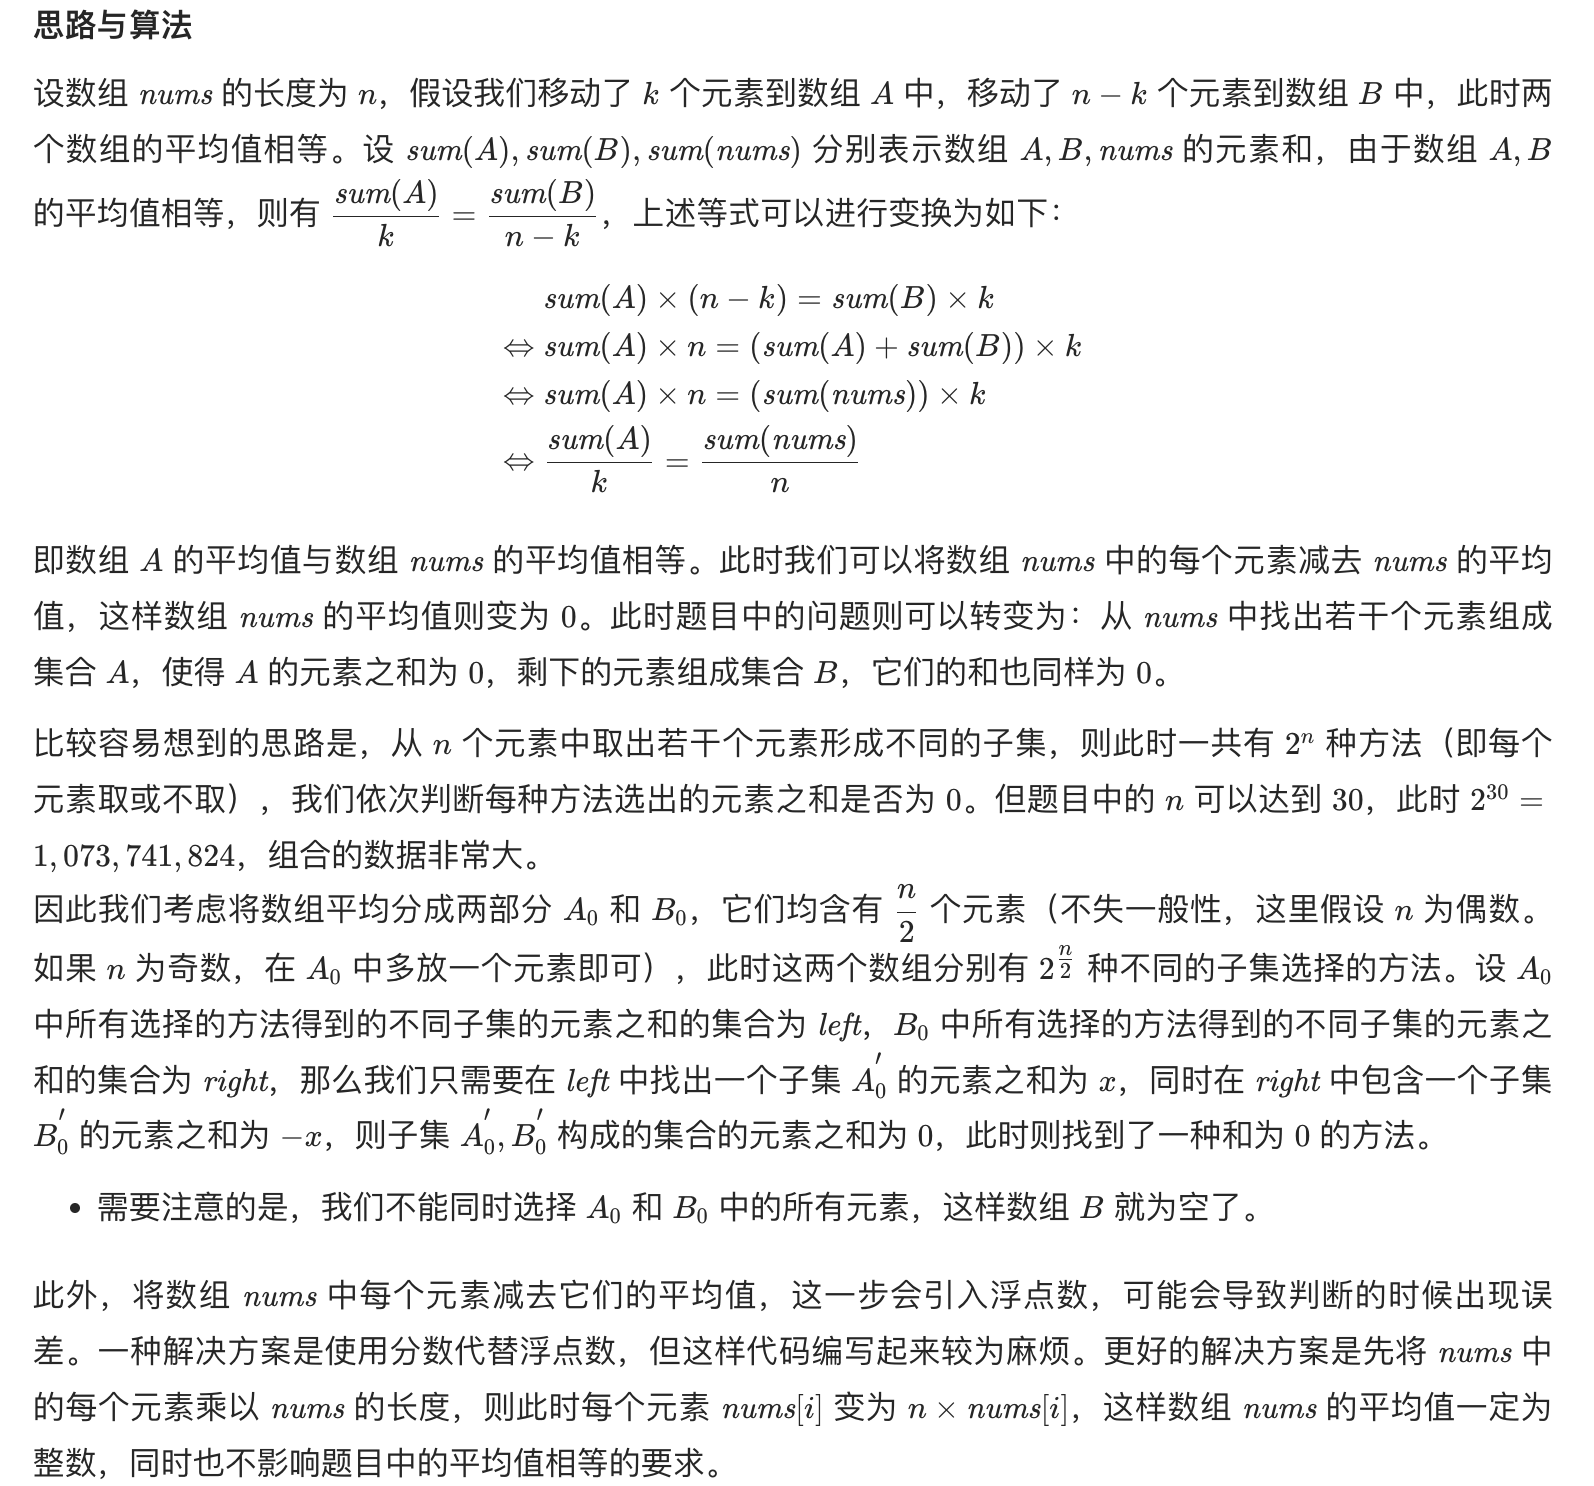
\includegraphics[width=.9\linewidth]{./pic/dp_20230414_202227.png}
\begin{minted}[fontsize=\scriptsize,linenos=false]{csharp}
// 第一种方法:原始,相对比较土。。。。。
public boolean splitArraySameAverage(int[] a) {
    if (a.length == 1) return false;
    int n = a.length, sum = Arrays.stream(a).sum(), m = n / 2;
    // 把原数组和变0, 并且不引入任何浮点数
    for (int i = 0; i < n; i++) a[i] = a[i] * n - sum;
    // // 把原数组分成两个大小最接近的数组【再说一遍:概念上的,并不真的需要物理上的拆分为两个数组。。。】
    // int [] l = Arrays.copyOfRange(a, 0, n/2); // 【L-inclusive, r-excluesive)
    // int [] r = Arrays.copyOfRange(a, n/2, n);
    // 求一个数组可能取得的和 sum 集合
    Set<Integer> lsum = new HashSet<>();
    for (int i = 1; i < (1 << m); i++) {
        int s = 0;
        for (int j = 0; j < m; j++) // 这里可能会遍历多了
            if (((i >> j) & 1) == 1) s += a[j];
// 【快速返回:】这里是可以优化提速的地方。左边非空集合和为0, 那么左边非空补集的和也一定为 0
        if (s == 0) return true; 
        lsum.add(s);
    }
    // 遍历:求右边数组可能取得的和 s,并一一去找左边是否存在和 -s
    int rsum = 0; // 先求右边的和:
    for (int i = m; i < n; i++) rsum += a[i];
    for (int i = 1; i < (1 << n - m); i++) {
        int s = 0;
        for (int j = m; j < n; j++) // 这里可能会遍历多了
            if (((i >> (j - m)) & 1) == 1) s += a[j];
        // if (s == 0 || lsum.contains(-s)) return true; // 【BUG:】
        if (s == 0 || s != rsum && lsum.contains(-s)) return true; // 【为什么 s != rsum 重要?】【3, 1】==》【2, -2】
    }
    return false;
}
\end{minted}
\begin{itemize}
\item 复杂度分析
\end{itemize}

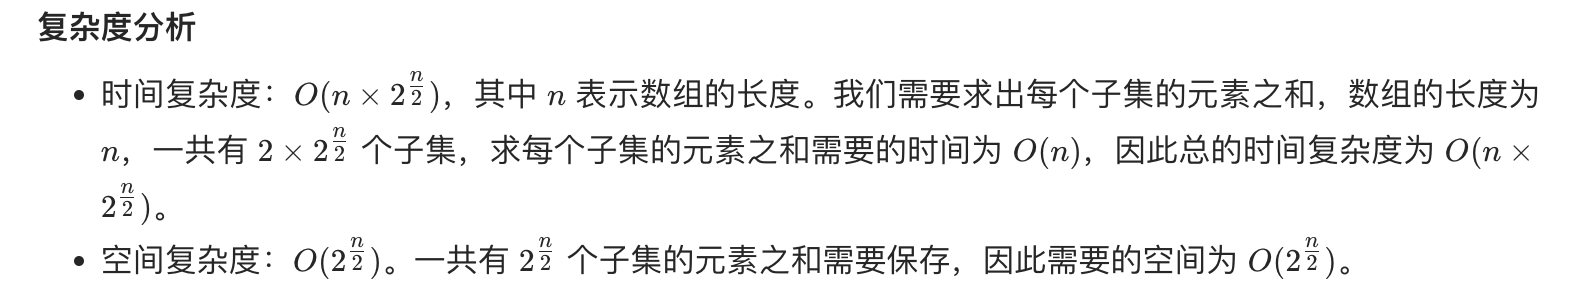
\includegraphics[width=.9\linewidth]{./pic/dp_20230414_202315.png}
\item 动态规划
\label{sec-1-4-1-2}

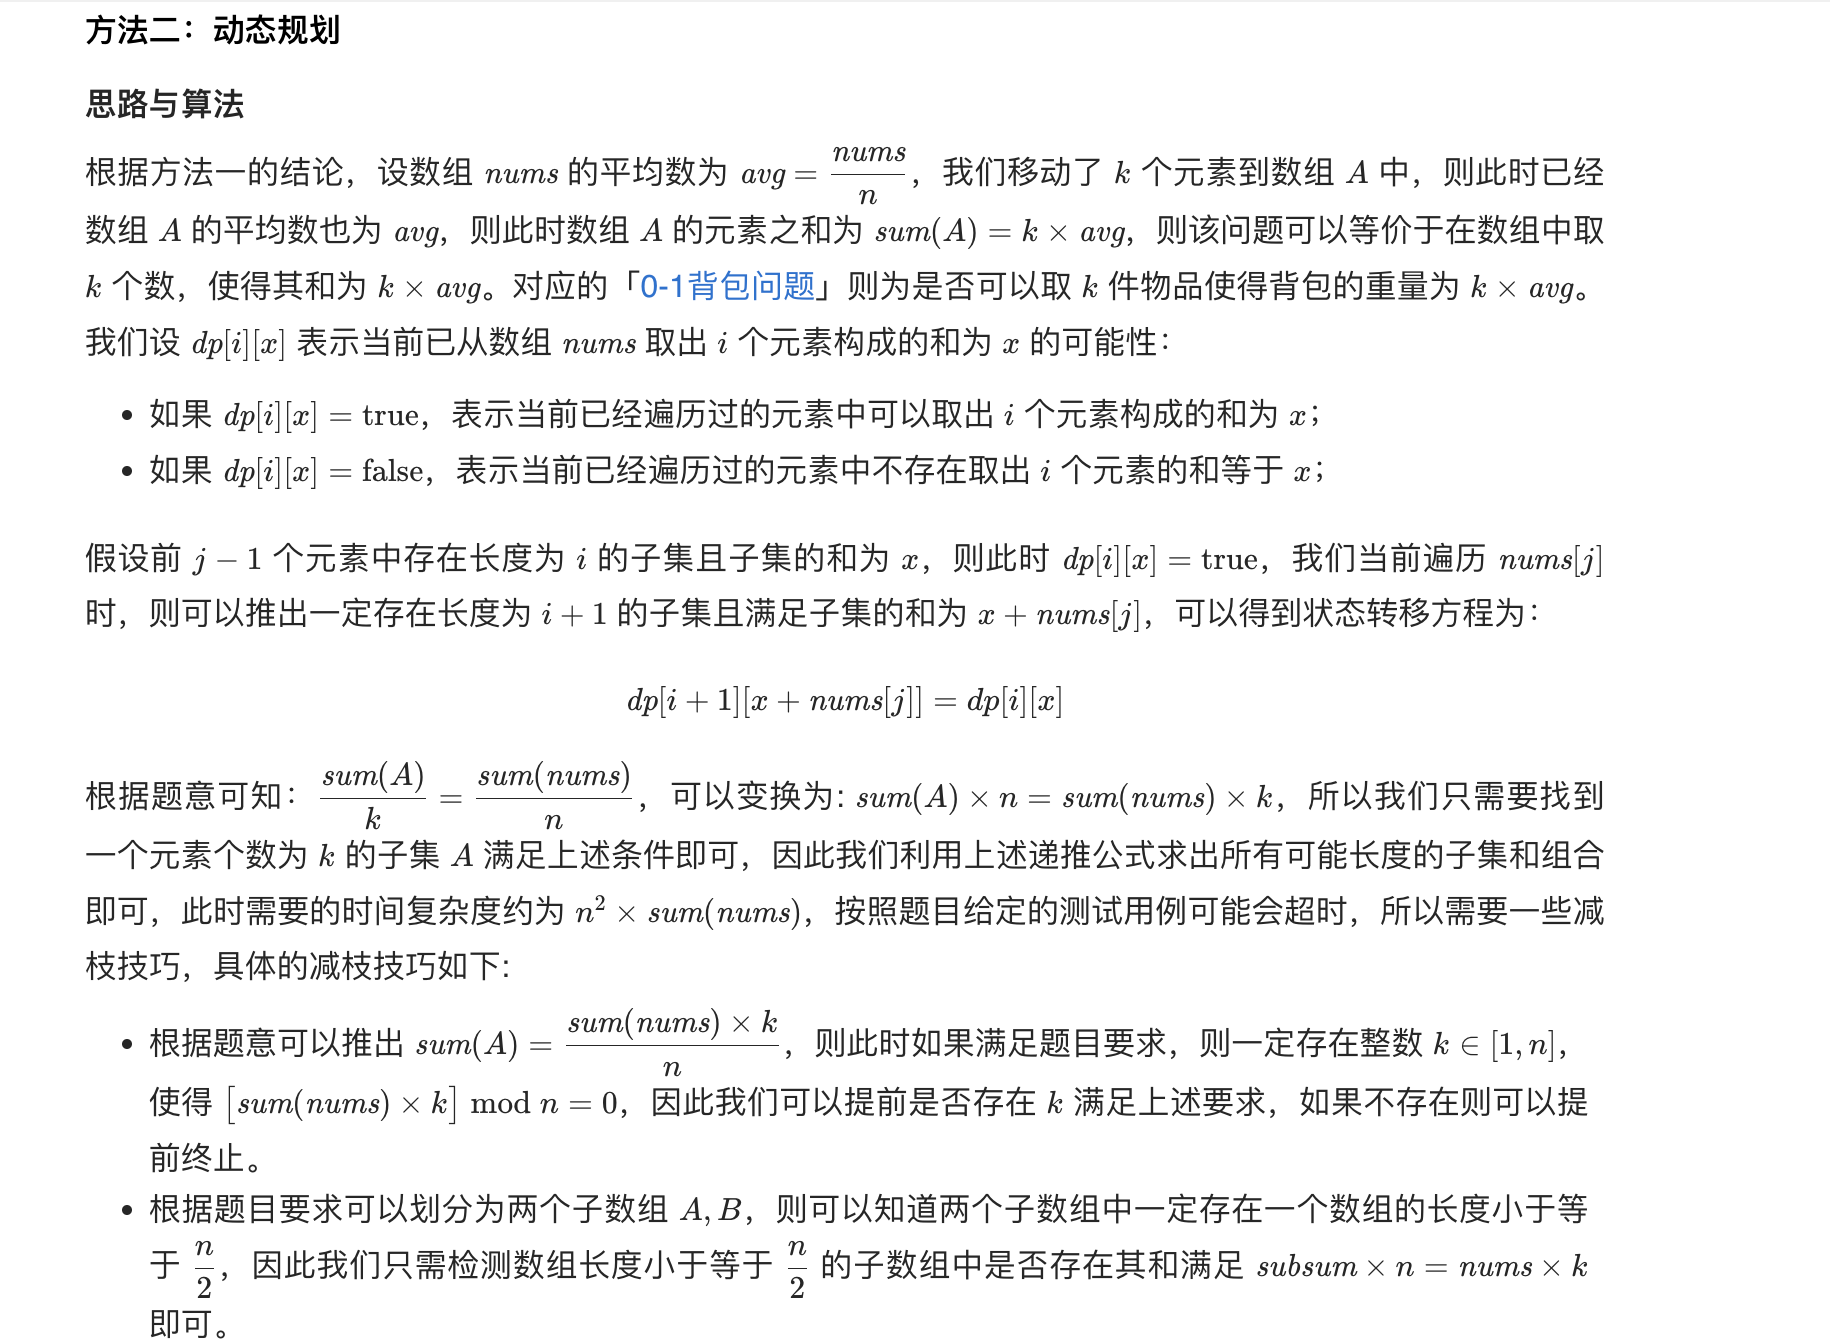
\includegraphics[width=.9\linewidth]{./pic/dp_20230414_202732.png}
\begin{minted}[fontsize=\scriptsize,linenos=false]{java}
public boolean splitArraySameAverage(int[] a) {
if (a.length == 1) return false;
int n = a.length, m = n / 2, sum = Arrays.stream(a).sum();
  boolean isPossible = false;
    for (int i = 1; i <= m; i++)
        if (sum * i % n == 0) {
            isPossible = true;
            break;
        }
    if (!isPossible) return false;
    Set<Integer> [] f = new HashSet [m+1];
    Arrays.setAll(f, z -> new HashSet<>());
    f[0].add(0);
    for (int v : a) 
        for (int i = m; i >= 1; i--) 
            for (int x : f[i-1]) {
                int cur = x + v;
                if (cur * n == sum * i) return true;
                f[i].add(cur);
            }
    return false;
}
\end{minted}
\begin{itemize}
\item 复杂度分析:
\end{itemize}

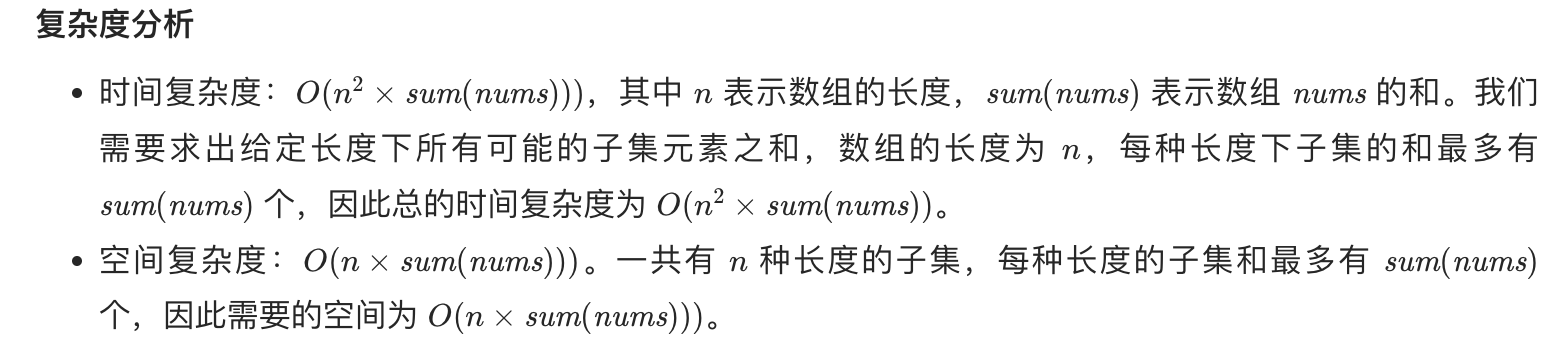
\includegraphics[width=.9\linewidth]{./pic/dp_20230414_202518.png}
\end{enumerate}
\subsection{805. Split Array With Same Average 【这里是怎么又重复了一遍?】需要合并一下}
\label{sec-1-4-2}
You are given an integer array nums.
You should move each element of nums into one of the two arrays A and B such that A and B are non-empty, and average(A) == average(B).
Return true if it is possible to achieve that and false otherwise.
Note that for an array arr, average(arr) is the sum of all the elements of arr over the length of arr.
\begin{minted}[fontsize=\scriptsize,linenos=false]{csharp}
    //     1)如果一个长度为n的数组可以被划分为A和B两个数组,我们假设A的长度小于B并且A的大小是k,那么:total_sum / n == A_sum / k == B_sum / (n - k),其中1 <= k <= n / 2。那么可以知道:A_sum = total_sum * k / n。由于A_sum一定是个整数,所以我们可以推导出total_sum * k % n == 0,那就是说,对于特定的total_sum和n而言,符合条件的k不会太多。这样我们在第一步中就首先验证是否存在符合条件的k,如果不存在就可以提前返回false。
    //     2)如果经过第一步的验证,发现确实有符合条件的k,那么我们在第二步中,就试图产生k个子元素的所有组合,并且计算他们的和。这里的思路就有点类似于背包问题了,vector<unordered_set<int>> sums,其中sums[i][j]表示A[0, i]这个子数组中的任意j个元素的所有可能和。可以得到递推公式是:sums[i][j] = sums[i - 1][j] "join" (sums[i][j - 1] + A[i]),其中等式右边的第一项表示这j个元素中不包含A[i],而第二项表示这j个元素包含A[i]。这样就可以采用动态规划的思路得到sums[n - 1][k]了(1 <= k <= n / 2)。
    // 3)有了sums[n - 1][k],我们就检查sums[n - 1][k]中是否包含(total_sum * k / n)。一旦发现符合条件的k,就返回true,否则就返回false。
    // 在递推公式中我们发现,sums[i][j]仅仅和sums[i - 1][j],sums[i][j - 1]有关,所以可以进一步将空间复杂度从O(n^2*M)降低到O(n*M),其中M是n中的所有元素的组合数(可能高达O(2^n))。时间复杂度为O(n^3*M)。
public boolean splitArraySameAverage(int[] nums) {
    int n = nums.length;
    int m = n / 2;
    int sum = Arrays.stream(nums).sum();
    boolean poss = false;
    for (int i = 1; i <= m; i++) {
        if (sum * i % n == 0) {
            poss = true;
            break;
        }
    }
    if (!poss) return false;
    List<Set<Integer>> ls = new ArrayList<>();
    for (int i = 0; i <= m; i++) 
        ls.add(new HashSet<Integer>());
    ls.get(0).add(0);    // 这种构建子序列和的方法,要学习一下
    for (int v : nums) { // for each element in A, we try to add it to sums[i] by joining sums[i - 1]
        for (int i = m; i >= 1; i--) {
            for (int t : ls.get(i-1)) {
                ls.get(i).add(t + v);
            }
        }
    }
    // System.out.println("ls.size(): " + ls.size());
    // for (int z = 0; z < ls.size(); ++z) {
    //     for (Integer x : ls.get(z))
    //         System.out.print(x + ", ");
    //     System.out.print("\n");
    //     System.out.print("\n ");
    // }
    for (int i = 1; i <= m; i++) {
        if (sum * i % n == 0 && ls.get(i).contains(sum * i / n))
            return true;
    }
    return false;
}
private boolean helper(int [] arr, int curSum, int cur, int start) {
    if (cur == 0) return curSum == 0;
    if (arr[start] > curSum / cur) return false;
    for (int i = start; i < arr.length - cur + 1; i++) {
        if (i > start && arr[i] == arr[i-1]) continue;
        if (helper(arr, curSum - arr[i], cur-1, i+1)) return true;
    }
    return false;
}
public boolean splitArraySameAverage(int[] nums) {
    int n = nums.length;
    int m = n / 2;
    int sum = Arrays.stream(nums).sum();
    boolean poss = false;
    for (int i = 1; i <= m; i++) {
        if (sum * i % n == 0) {
            poss = true;
            break;
        }
    }
    if (!poss) return false;
    Arrays.sort(nums);
    for (int i = 1; i <= m; i++) 
        if (sum * i % n == 0 && helper(nums, sum * i / n, i, 0)) return true;
    return false;
}
bool splitArraySameAverage(vector<int>& A) {  // https://www.cnblogs.com/grandyang/p/10285531.html
    int n = A.size(), m = n / 2, sum = accumulate(A.begin(), A.end(), 0);
    bool possible = false;
    for (int i = 1; i <= m && !possible; ++i) {
        if (sum * i % n == 0) possible = true;
    }
    if (!possible) return false;
    bitset<300001> bits[m + 1] = {1};
    for (int num : A) {
        for (int i = m; i >= 1; --i) {
            bits[i] |= bits[i - 1] << num;
        }
    }
    for (int i = 1; i <= m; ++i) {
        if (sum * i % n == 0 && bits[i][sum * i / n]) return true;
    }
    return false;
}
\end{minted}
\subsection{1235. Maximum Profit in Job Scheduling - Hard}
\label{sec-1-4-3}
We have n jobs, where every job is scheduled to be done from startTime[i] to endTime[i], obtaining a profit of profit[i].

You're given the startTime, endTime and profit arrays, return the maximum profit you can take such that there are no two jobs in the subset with overlapping time range.

If you choose a job that ends at time X you will be able to start another job that starts at time X.
\begin{enumerate}
\item 解题思路与分析
\label{sec-1-4-3-1}

Sort the elements by starting time, then define the dp[i] as the maximum profit taking elements from the suffix starting at i.

Use binarySearch (lower\_bound/upper\_bound on C++) to get the next index for the DP transition.- 

\begin{minted}[fontsize=\scriptsize,linenos=false]{csharp}
// 目标:在最接近自己startime的endtime里得到最大的proft前缀
// 维护一个递增的endtime序列
// 该序列同时记录在此endtime下的最大profit
// 按递增endtime遍历工作
// 如果本次工作后profit比更早的endtime下的更多,就把这个工作记进去,不然做个p
// 因为升序,所以还能二分查找。exciting!
public int jobScheduling(int[] startTime, int[] endTime, int[] profit) { // 这个前后的时间点总是没能确定,所以思路不清晰
    int n = startTime.length;
    List<int []> map = new ArrayList<>();
    for (int i = 0; i < startTime.length; i++) 
        map.add(new int [] {startTime[i], endTime[i], profit[i]});
    Collections.sort(map, (a, b) -> a[0] - b[0]);
    for (int [] zz : map) 
        System.out.println(Arrays.toString(zz));

    int [] dp = new int [n];
    dp[n-1] = map.get(n-1)[2]; // 反向逆序遍历的优点:遍历过的时间点一定在当前事件之后,只有选与不选当前事件两种策略中取最优解
    int j = 0;
    for (int i = n-2; i >= 0; i--) {
        j = binarySearchNext(i+1, map);
        // j = getNext(i, map);
        dp[i] = Math.max(dp[i+1], (j == -1 ? 0 : dp[j]) + map.get(i)[2]);
    }
    return dp[0];
}
private int getNext(int idx, List<int []> ll) {
    for (int i = idx+1; i < ll.size(); i++) 
        if (ll.get(i)[0] >= ll.get(idx)[1]) return i;
    return -1;
}
private int binarySearchNext(int x, List<int []> ll) { // 这里居然写出bug来了 // bug todo
    int l = x + 1, r = ll.size()-1, v = ll.get(x)[1], ans = -1; // x end time
    while (l <= r) {
        int m = l + (r - l) / 2;
        if (ll.get(m)[0] >= v) {
            ans = m;
            r = m-1;
        } else l = m+1;
    }
    // return l < ll.size() && ll.get(l)[0] >= v ? l : -1;
    return ans;
}
\end{minted}
\end{enumerate}
\subsection{2008. Maximum Earnings From Taxi - Medium}
\label{sec-1-4-4}
There are n points on a road you are driving your taxi on. The n points on the road are labeled from 1 to n in the direction you are going, and you want to drive from point 1 to point n to make money by picking up passengers. You cannot change the direction of the taxi.

The passengers are represented by a 0-indexed 2D integer array rides, where rides[i] = [starti, endi, tipi] denotes the ith passenger requesting a ride from point starti to point endi who is willing to give a tipi dollar tip.

For each passenger i you pick up, you earn endi - starti + tipi dollars. You may only drive at most one passenger at a time.

Given n and rides, return the maximum number of dollars you can earn by picking up the passengers optimally.

Note: You may drop off a passenger and pick up a different passenger at the same point.
\begin{enumerate}
\item 解题思路与分析
\label{sec-1-4-4-1}
\begin{minted}[fontsize=\scriptsize,linenos=false]{csharp}
public long maxTaxiEarnings(int n, int[][] rides) {
    Arrays.sort(rides, (a, b)-> (a[0] != b[0] ? a[0] - b[0] : a[1] - b[1]));
    Map<Integer, Set<int []>> m = new HashMap<>();
    for (int [] r : rides) 
        m.computeIfAbsent(r[1], z -> new HashSet<>()).add(r);
    long [] dp = new long [n+1];
    for (int i = 1; i <= n; i++) {
        dp[i] = dp[i-1];
        if (m.containsKey(i)) 
            for (int [] r : m.get(i)) 
                dp[r[1]] = Math.max(dp[r[1]], dp[r[0]] + r[1] - r[0] + r[2]);
    }
    return dp[n];
}
\end{minted}
\item 解题思路与分析
\label{sec-1-4-4-2}
\begin{minted}[fontsize=\scriptsize,linenos=false]{csharp}
// Similar to 1235. Maximum Profit in Job Scheduling
// Sort by the end time to get non-overlapping intervals.
// Use the treemap to find the previous ride before the current ride.
public long maxTaxiEarnings(int n, int[][] rides) {
    if (rides == null || rides.length == 0) return 0;
    for (int[] r : rides) 
        r[2] = r[1] - r[0] + r[2];
    Arrays.sort(rides, (a, b) -> (a[1] - b[1]));
    TreeMap<Long, Long> map = new TreeMap<>();
    map.put((long)0, (long)0); 
    for (int[] r : rides) {
        long cur = map.floorEntry((long)r[0]).getValue() + r[2];
        if (cur > map.lastEntry().getValue()) {
            map.put((long)r[1], cur);
        }
    }
    return map.lastEntry().getValue();
}
\end{minted}
\end{enumerate}

\subsection{1713. Minimum Operations to Make a Subsequence - Hard LIS 经曲题型,需要吃透}
\label{sec-1-4-5}
You are given an array target that consists of distinct integers and another integer array arr that can have duplicates.

In one operation, you can insert any integer at any position in arr. For example, if arr = [1,4,1,2], you can add 3 in the middle and make it [1,4,3,1,2]. Note that you can insert the integer at the very beginning or end of the array.

Return the minimum number of operations needed to make target a subsequence of arr.

A subsequence of an array is a new array generated from the original array by deleting some elements (possibly none) without changing the remaining elements' relative order. For example, [2,7,4] is a subsequence of [4,2,3,7,2,1,4] (the underlined elements), while [2,4,2] is not.
\begin{enumerate}
\item 解题思路与分析
\label{sec-1-4-5-1}
\begin{minted}[fontsize=\scriptsize,linenos=false]{csharp}
public int minOperations(int[] t, int[] a) {
    int n = t.length;
    Map<Integer, Integer> m = new HashMap<Integer, Integer>();
    for (int i = 0; i < n; ++i) 
        m.put(t[i], i);
    List<Integer> d = new AayList<Integer>();
    for (int val : a) 
        if (m.containsKey(val)) {
            int idx = m.get(val);
            int it = binarySearch(d, idx);
            if (it != d.size()) 
                d.set(it, idx);
            else 
                d.add(idx);
        }
    return n - d.size();
}
public int binarySearch(List<Integer> li, int t) {
    int size = li.size();
    if (size == 0 || li.get(size - 1) < t) 
        return size;
    int low = 0, high = size - 1;
    while (low < high) {
        int mid = (high - low) / 2 + low;
        if (li.get(mid) < t) 
            low = mid + 1;
        else 
            high = mid;
    }
    return low;
}
\end{minted}
\end{enumerate}
\subsection{1879. Minimum XOR Sum of Two Arrays - Hard}
\label{sec-1-4-6}
You are given two integer arrays nums1 and nums2 of length n.

The XOR sum of the two integer arrays is (nums1\footnotemark[1]{} XOR nums2\footnotemark[1]{}) + (nums1\footnotemark[2]{} XOR nums2\footnotemark[2]{}) + \ldots{} + (nums1[n - 1] XOR nums2[n - 1]) (0-indexed).

For example, the XOR sum of [1,2,3] and [3,2,1] is equal to (1 XOR 3) + (2 XOR 2) + (3 XOR 1) = 2 + 0 + 2 = 4.
Rearrange the elements of nums2 such that the resulting XOR sum is minimized.

Return the XOR sum after the rearrangement.
\begin{enumerate}
\item 解题思路与分析
\label{sec-1-4-6-1}
\begin{minted}[fontsize=\scriptsize,linenos=false]{csharp}
// 参考 n 的范围 [1, 14],可状态压缩后结合动态规划方法求解。
// 设计一个动态规划数组 dp[1 << n],
// 对每个 dp[i],若 i 的二进制表示中 1 的个数为 num, 1 的位置为 k1, k2, …, knum,
//     dp[i] 表示 nums1 的前 num 个数和 nums2 第 k1, k2, …, knum 个数的最小异或值之和。
public int minimumXORSum(int[] a, int[] b) { // 就像前面有题可以一个字母一个字母地match寻找最少单词个数,这里有每增加一个数对的异或都优化结果的细节在
    int n = a.length, r = 1 << n;
    int [] dp = new int [r]; // dp[]: 这个设计奇特,最开始居然没能想起来,要熟悉起来
    Arrays.fill(dp, Integer.MAX_VALUE);
    dp[0] = 0; // 每一个数对取最小值结果的优化是从0开始
    for (int i = 0; i < r; i++) 
        for (int j = 0; j < n; j++) 
            if (((i >> j) & 1) == 1)
                dp[i] = Math.min(dp[i], dp[i ^ (1 << j)] + (a[Integer.bitCount(i)-1] ^ b[j])); 
                // dp[i] = Math.min(dp[i], dp[i ^ (1 << j)] + a[Integer.bitCount(i)-1] ^ b[j]); // BUG: ^ 位操作符优先给很低,需要()起来
    return dp[r-1];
}
\end{minted}
\begin{itemize}
\item 当这类题写熟悉了,要写得横看成岭侧成峰,远近高低各不同,要写得随心所欲,想怎么写都能写得出来才可以
\end{itemize}
\begin{minted}[fontsize=\scriptsize,linenos=false]{csharp}
public int minimumXORSum(int[] a, int[] b) {
    int n = a.length, r = 1 << n;
    int [] dp = new int [r]; 
    Arrays.fill(dp, Integer.MAX_VALUE);
    for (int i = 0; i < n; i++) 
        dp[1 << i] = a[0] ^ b[i];
    int [] cnt = new int [r];
    for (int i = 0; i < r; i++)
        cnt[i] = Integer.bitCount(i);
    for (int i = 1; i < n; i++) 
        for (int j = r-1; j > 0; j--) { // 为避免产生赃数据,这里需要倒序遍历
            if (dp[j] == Integer.MAX_VALUE) continue;
            if (cnt[j] == i) // 原状态的 1 的个数 为 i 个,可以进行状态转移
                for (int k = 0; k < n; k++) 
                    if (((j >> k) & 1) == 0 && (j | (1 << k)) < r) // 遍历所有的位,碰到 state 0 的位置可以放一个异或
                        dp[j | (1 << k)] = Math.min(dp[j | (1 << k)], dp[j] + (a[i] ^ b[k])); // 新产生的数据向后覆盖
        }
    return dp[r-1];
}
\end{minted}
\end{enumerate}

\subsection{1883. Minimum Skips to Arrive at Meeting On Time - Hard}
\label{sec-1-4-7}
You are given an integer hoursBefore, the number of hours you have to travel to your meeting. To arrive at your meeting, you have to travel through n roads. The road lengths are given as an integer array dist of length n, where dist[i] describes the length of the ith road in kilometers. In addition, you are given an integer speed, which is the speed (in km/h) you will travel at.

After you travel road i, you must rest and wait for the next integer hour before you can begin traveling on the next road. Note that you do not have to rest after traveling the last road because you are already at the meeting.

For example, if traveling a road takes 1.4 hours, you must wait until the 2 hour mark before traveling the next road. If traveling a road takes exactly 2 hours, you do not need to wait.
However, you are allowed to skip some rests to be able to arrive on time, meaning you do not need to wait for the next integer hour. Note that this means you may finish traveling future roads at different hour marks.

For example, suppose traveling the first road takes 1.4 hours and traveling the second road takes 0.6 hours. Skipping the rest after the first road will mean you finish traveling the second road right at the 2 hour mark, letting you start traveling the third road immediately.
Return the minimum number of skips required to arrive at the meeting on time, or -1 if it is impossible.
\begin{enumerate}
\item 解题思路与分析
\label{sec-1-4-7-1}
\begin{minted}[fontsize=\scriptsize,linenos=false]{csharp}
// dp[i][j] 表示途径 i 条道路跳过 j 次休息情况下的最小用时,遍历过程中根据上一道路是否休息选取最小值,结合状态转移方程求解。
public int minSkips(int [] dist, int speed, int hoursBefore) {
    int n = dist.length;
    double [][] dp = new double [n+1][n+1]; // dp[i][j]: 途经i条道路,跳过j次休息下的最小用时
    for (int i = 0; i <= n; i++) 
        Arrays.fill(dp[i], Integer.MAX_VALUE);
    dp[0][0] = 0;
    double eps = 1e-8; // eps用于避免浮点数计算误差导致向上取整后出现错误,inf作为最大值初始化动态规划数组
    for (int i = 1; i <= n; i++) {
        double t = (double)dist[i-1] / speed;       // 第i条道路耗时
        dp[i][0] = Math.ceil(dp[i-1][0] - eps) + t; // 单独计算不跳过休息时的值
        dp[i][i] = dp[i-1][i-1] + t;                // 单独计算跳过所有休息时的值
        for (int j = i-1; j > 0; j--) // 根据上一条路是否休息,来优化最小值
            dp[i][j] = Math.min(Math.ceil(dp[i-1][j] - eps) + t, dp[i-1][j-1] + t);
    }
    for (int i = 0; i <= n; i++) 
        if (dp[n][i] <= hoursBefore + eps) return i;
    return -1;
}
\end{minted}
\end{enumerate}

\subsection{1786. Number of Restricted Paths From First to Last Node - Dijkstra算法}
\label{sec-1-4-8}
There is an undirected weighted connected graph. You are given a positive integer n which denotes that the graph has n nodes labeled from 1 to n, and an array edges where each edges[i] = [ui, vi, weighti] denotes that there is an edge between nodes ui and vi with weight equal to weighti.
A path from node start to node end is a sequence of nodes [z0, z1, z2, \ldots{}, zk] such that z0 = start and zk = end and there is an edge between zi and zi+1 where 0 <= i <= k-1.
The distance of a path is the sum of the weights on the edges of the path. Let distanceToLastNode(x) denote the shortest distance of a path between node n and node x. A restricted path is a path that also satisfies that distanceToLastNode(zi) > distanceToLastNode(zi+1) where 0 <= i <= k-1.
Return the number of restricted paths from node 1 to node n. Since that number may be too large, return it modulo 109 + 7.
\begin{minted}[fontsize=\scriptsize,linenos=false]{csharp}
public int countRestrictedPaths(int n, int[][] edges) {
    this.n = n;
    for (int [] e : edges) {
        adj.computeIfAbsent(e[0], z -> new HashMap<>()).put(e[1], e[2]);
        adj.computeIfAbsent(e[1], z -> new HashMap<>()).put(e[0], e[2]);
    }
    dist = new int [n+1];
    Arrays.fill(dist, Integer.MAX_VALUE);
    dist[n] = 0;
    dijkstra();
    dp = new int [n+1];
    Arrays.fill(dp, -1);
    return (int)dfs(1);
}
HashMap<Integer, Map<Integer, Integer>> adj = new HashMap<>();
int mod = (int)1e9 + 7;
int [] dist;
int [] dp;
int n;
private long dfs(int u) {
    if (u == n) return 1;
    if (dp[u] != -1) return dp[u];
    long ans = 0;
    Map<Integer, Integer> tmp = adj.get(u);
    if (tmp != null) 
        for (Integer v : tmp.keySet()) 
            if (dist[u] > dist[v])
                ans = (ans + dfs(v)) % mod;
    return dp[u] = (int)ans;
}
private void dijkstra() {
    // Queue<int []> q = new LinkedList<>(); // tle 
    Queue<int []> q = new PriorityQueue<>((a, b)->a[1] - b[1]); // 狠重要
    q.offer(new int [] {n, 0});
    while (!q.isEmpty()) {
        int [] u = q.poll();
        if (dist[u[0]] < u[1]) continue; // 狠重要
        Map<Integer, Integer> tmp = adj.get(u[0]);
        if (tmp == null) continue;
        for (Integer v : tmp.keySet()) 
            if (u[1] + tmp.get(v) < dist[v]) {
                dist[v] = u[1] + tmp.get(v);
                q.offer(new int [] {v, dist[v]});
            }
    }
}
\end{minted}

\subsection{1911. Maximum Alternating Subsequence Sum - Medium todo: 还需要总结题解}
\label{sec-1-4-9}
The alternating sum of a 0-indexed array is defined as the sum of the elements at even indices minus the sum of the elements at odd indices.

For example, the alternating sum of [4,2,5,3] is (4 + 5) - (2 + 3) = 4.
Given an array nums, return the maximum alternating sum of any subsequence of nums (after reindexing the elements of the subsequence).

A subsequence of an array is a new array generated from the original array by deleting some elements (possibly none) without changing the remaining elements' relative order. For example, [2,7,4] is a subsequence of [4,2,3,7,2,1,4] (the underlined elements), while [2,4,2] is not.
\begin{enumerate}
\item 解题思路与分析: DP
\label{sec-1-4-9-1}

设计两个长整数 evenDp 和 oddDp,分别记录上一元素为偶数下标、奇数下标时当前的最大交替和。根据是否添加当前元素,状态转移方程为:

evenDp = Math.max(上一 evenDp, 上一 oddDp + 当前元素)

oddDp = Math.max(上一 oddDp, 上一 evenDp + 当前元素)

最终得到的 evenDp 即为最大交替和。

\begin{minted}[fontsize=\scriptsize,linenos=false]{csharp}
public long maxAlternatingSum(int[] a) {
    long odd = 0, evn = a[0]; // 上一元素为偶数下标、奇数下标时的最大交替和
    for (int i = 1; i < a.length; i++) {
        evn = Math.max(evn, odd + a[i]); // 偶数下标交替和转移
        odd = Math.max(odd, evn - a[i]); // 奇数下标交替和转移
    }
    return evn;
}
\end{minted}
\item 解题思路与分析: 最大股票收益
\label{sec-1-4-9-2}
参考Leetcode题解,发现有一个方法很巧妙。将样例[6,2,1,2,4,5]转化为[0,6,2,1,2,4,5],那么题面就转化为模拟股票交易,数组中的数为股票价格,index为天数。

你可以在第i天买入股票,第j天卖出股票,其中i<=j。

那么其实我们可以用上帝视角来看,只要股票价格后一天比当天高,我们就当天买入,后一天卖出。

那么就如下所示:
\begin{minted}[fontsize=\scriptsize,linenos=false]{csharp}
买入    卖出    收益
第0天   第1天   6-0=6
第3天   第4天   2-1=1
第4天   第5天   4-2=2
第5天   第6天   5-4=1
\end{minted}

那么总收益为6+1+2+1=10,即6-0+2-1+4-2+5-4,抵消之后就是6-1+5,就是样例中的最优子序列[6,1,5]\textasciitilde{}
\begin{minted}[fontsize=\scriptsize,linenos=false]{csharp}
public long maxAlternatingSum(int[] a) {
    int [] b = new int [a.length+1];
    System.arraycopy(a, 0, b, 1, a.length);
    long ans = 0;
    for (int i = 1; i < b.length; i++) 
        if (b[i] - b[i-1] > 0) ans += b[i] - b[i-1];
    return ans;
}
\end{minted}
\end{enumerate}

\subsection{1928. Minimum Cost to Reach Destination in Time - Hard}
\label{sec-1-4-10}
There is a country of n cities numbered from 0 to n - 1 where all the cities are connected by bi-directional roads. The roads are represented as a 2D integer array edges where edges[i] = [xi, yi, timei] denotes a road between cities xi and yi that takes timei minutes to travel. There may be multiple roads of differing travel times connecting the same two cities, but no road connects a city to itself.

Each time you pass through a city, you must pay a passing fee. This is represented as a 0-indexed integer array passingFees of length n where passingFees[j] is the amount of dollars you must pay when you pass through city j.

In the beginning, you are at city 0 and want to reach city n - 1 in maxTime minutes or less. The cost of your journey is the summation of passing fees for each city that you passed through at some moment of your journey (including the source and destination cities).

Given maxTime, edges, and passingFees, return the minimum cost to complete your journey, or -1 if you cannot complete it within maxTime minutes.
\begin{enumerate}
\item 解题思路与分析
\label{sec-1-4-10-1}
\begin{minted}[fontsize=\scriptsize,linenos=false]{csharp}
// 设计一个动态规划数组 dp[maxTime + 1][n],其中 dp[t][i] 表示第 t 分钟到达城市 i 时的最少费用,则状态转移方程为:
// dp[t][c1] = Math.min(dp[t][c1], dp[t - time][c2] + passingFees[c1])
// dp[t][c2] = Math.min(dp[t][c2], dp[t - time][c1] + passingFees[c2])
public int minCost(int maxTime, int[][] edges, int[] passingFees) {
    int n = passingFees.length;
    int [][] dp = new int [maxTime+1][n];
    for (int i = 0; i <= maxTime; i++) 
        Arrays.fill(dp[i], Integer.MAX_VALUE / 2);
    dp[0][0] = passingFees[0];
    for (int t = 0; t <= maxTime; t++) 
        for (int [] e : edges) {
            if (e[2] > t) continue;
            int u = e[0], v = e[1], time = e[2];
            dp[t][u] = Math.min(dp[t][u], dp[t-time][v] + passingFees[u]); // v --> u
            dp[t][v] = Math.min(dp[t][v], dp[t-time][u] + passingFees[v]); // u --> v
        }
    int ans = Integer.MAX_VALUE / 2;
    for (int i = 1; i <= maxTime; i++)
        ans = Math.min(ans, dp[i][n-1]);
    return ans == Integer.MAX_VALUE / 2 ? -1 : ans;
}
\end{minted}
\end{enumerate}

\subsection{730. Count Different Palindromic Subsequences - Hard}
\label{sec-1-4-11}
Given a string s, return the number of different non-empty palindromic subsequences in s. Since the answer may be very large, return it modulo 109 + 7.

A subsequence of a string is obtained by deleting zero or more characters from the string.

A sequence is palindromic if it is equal to the sequence reversed.

Two sequences a1, a2, \ldots{} and b1, b2, \ldots{} are different if there is some i for which ai != bi.

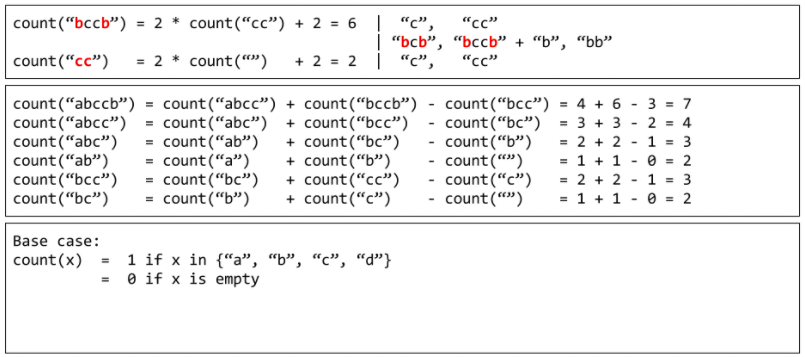
\includegraphics[width=.9\linewidth]{./pic/palindromSubSeq.png}

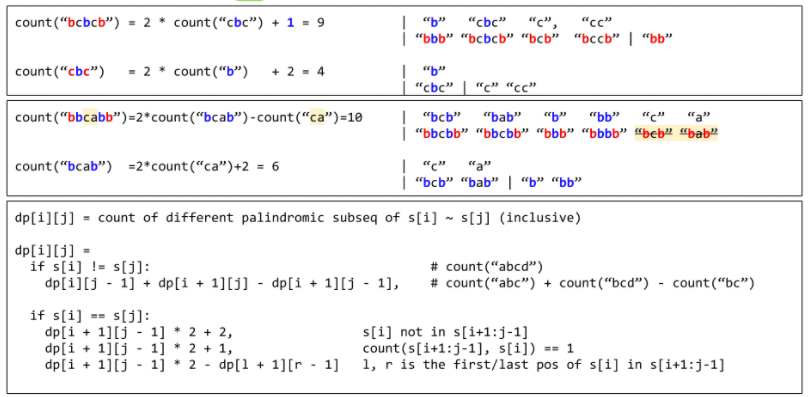
\includegraphics[width=.9\linewidth]{./pic/palindromSubSeq2.png}

\begin{minted}[fontsize=\scriptsize,linenos=false]{csharp}
private int dfs(char[] s, int i, int j) {
    if (i > j) return 0;
    if (i == j) return 1;
    if (dp[i][j] > 0) return dp[i][j];
    long ans = 0;
    if (s[i] == s[j]) {
        ans += dfs(s, i + 1, j - 1) * 2;
        int l = i + 1;
        int r = j - 1;
        while (l <= r && s[l] != s[i]) ++l;
        while (l <= r && s[r] != s[i]) --r;
        if (l > r) ans += 2;
        else if (l == r) ans += 1;
        else ans -= dfs(s, l + 1, r - 1);
    } else 
        ans = dfs(s, i, j - 1) + dfs(s, i + 1, j) - dfs(s, i + 1, j - 1);
    return dp[i][j] = (int)((ans + mod) % mod);
}
private static final int mod = (int)1e9 + 7;
private int [][] dp;
public int countPalindromicSubsequences(String S) {
    int n = S.length();
    dp = new int[n][n];
    return dfs(S.toCharArray(), 0, n - 1);
}
\end{minted}
\begin{itemize}
\item dp
\end{itemize}
\begin{minted}[fontsize=\scriptsize,linenos=false]{csharp}
public int countPalindromicSubsequences(String s) {
    int n = s.length();
    int mod = (int)1e9 + 7;
    char [] arr = s.toCharArray();
    long [][] dp = new long [n][n];
    for (int i = 0; i < n; i++) 
        dp[i][i] = 1;
    for (int len = 1; len <= n; len++) {
        for (int i = 0; i+len < n; i++) {
            int j = i + len;
            if (arr[i] == arr[j]) {
                dp[i][j] = dp[i+1][j-1] * 2;
                int l = i+1;
                int r = j-1;
                while (l <= r && arr[l] != arr[i]) ++l;
                while (l <= r && arr[r] != arr[i]) --r;
                if (l == r) dp[i][j] += 1;
                else if (l > r) dp[i][j] += 2;
                else dp[i][j] -= dp[l+1][r-1];
            } else dp[i][j] = dp[i][j-1] + dp[i+1][j] - dp[i+1][j-1];
            dp[i][j] = (dp[i][j] + mod) % mod;
        }
    }
    return (int)dp[0][n-1];
}
\end{minted}

\subsection{1125. Smallest Sufficient Team - Hard 这个题要多写几遍}
\label{sec-1-4-12}
In a project, you have a list of required skills req\_skills, and a list of people. The ith person people[i] contains a list of skills that the person has.

Consider a sufficient team: a set of people such that for every required skill in req\_skills, there is at least one person in the team who has that skill. We can represent these teams by the index of each person.

For example, team = [0, 1, 3] represents the people with skills people\footnotemark[1]{}, people\footnotemark[2]{}, and people\footnote{DEFINITION NOT FOUND.}.
Return any sufficient team of the smallest possible size, represented by the index of each person. You may return the answer in any order.

It is guaranteed an answer exists.
\begin{minted}[fontsize=\scriptsize,linenos=false]{csharp}
// 强行剪枝: 收集到的size >= 目前的结果,直接return;
// 这题的思路就是先把skill 和set of people建立好,
// 然后去用skill set做backtracking收集,如果temp team的size大于结果,直接return,否则update结果,
// 这里有个小tricky的地方,就是如果people是新人,加入之后dfs,backtracking的时候,要判断如果是新人,则remove,否则不remove;
private void dfs(String[] req_skills, HashSet<Integer> team, int idx) {
    if (team.size() >= minTeamSize) return; // 强行剪枝: 收集到的size >= 目前的结果,直接return;
    if (idx == req_skills.length) {
        minTeamSize = team.size();
        resTeam = new HashSet<Integer>(team);
        return;
    }
    boolean isNewPerson = false;
    for (int people : map.get(req_skills[idx])) {
        isNewPerson = team.add(people);
        dfs(req_skills, team, idx + 1);
        if (isNewPerson)
            team.remove(people);
    }
}
HashMap<String, Set<Integer>> map;
Set<Integer> resTeam; 
int minTeamSize;
public int[] smallestSufficientTeam(String[] req_skills, List<List<String>> people) {
    minTeamSize = people.size();
    this.map = new HashMap<>(); 
    for (int i = 0; i < minTeamSize; i++) 
        for (String skill: people.get(i)) 
            map.computeIfAbsent(skill, k -> new HashSet<Integer>()).add(i);
    this.resTeam = new HashSet<Integer>();
    dfs(req_skills, new HashSet<Integer>(), 0);
    int [] res = new int[resTeam.size()];     
    int idx = 0;
    for (int person : resTeam) 
        res[idx++] = person;
    return res;
}
\end{minted}
\begin{itemize}
\item Java soution using Bit DP 10ms
\end{itemize}
\begin{minted}[fontsize=\scriptsize,linenos=false]{csharp}
public int[] smallestSufficientTeam(String[] req_skills, List<List<String>> people) {
    int n = req_skills.length, range = 1 << n, cur, idx;
    Map<String, Integer> idxMap = new HashMap<>();
    for (int i = 0; i < n; i++) 
        idxMap.put(req_skills[i], i);
    long [] dp = new long [range]; // 每个bit位实际存了构成答案最小组的各成员的下标, 60个人, long
    int [] cnt = new int [range];
    Arrays.fill(cnt, Integer.MAX_VALUE);
    cnt[0] = 0;
    for (int i = 0; i < people.size(); i++) {
        List<String> l = people.get(i);
        cur = 0;
        for (String skill : l) 
            if (idxMap.containsKey(skill))
                cur |= 1 << idxMap.get(skill);
        for (int j = range-1; j > 0; j--) {
            idx = (j & cur) ^ j; // 由其它人所构成的拥有j的这些种技能的子集/ j的这些种技能可以由j一个人来替换(其它可能需要很多人才能最终拥有这些技能)
            if (cnt[idx] != Integer.MAX_VALUE && cnt[j] > cnt[idx] + 1) {
                cnt[j] = cnt[idx] + 1;
                dp[j] = dp[idx] | (1L << i); // at most 60 people
            }
        }
    }
    int [] res = new int[cnt[range-1]];
    long preRes = dp[range-1]; // 5 people: 11111, 1111, 111, 11, 1
    int valIdx = 0;
    long val = 0;
    idx = 0;
    while (preRes != 0) {
        val = preRes & 1;
        if (val == 1) res[idx++] = valIdx;
        preRes >>= 1;
        valIdx++;
    }
    return res;
}
\end{minted}
\begin{itemize}
\item DFS + Memorizaion (A real O(2\^{}skill * people) Solution) Java 8ms
\begin{itemize}
\item \url{https://leetcode.com/problems/smallest-sufficient-team/discuss/1011135/DFS-\%2B-Memorizaion}-(A-real-O(2skill-*-people)-Solution)-Java-8ms
\end{itemize}
\end{itemize}
\begin{minted}[fontsize=\scriptsize,linenos=false]{csharp}
List<Integer> minComb;
int[] peopleSkillMasks;
Integer[] memo;  // 这个方法确实快一点儿
int[] nextPerson;
int n;
public int[] smallestSufficientTeam(String[] req_skills, List<List<String>> people) {
    // 1. some preprocess to get bitmask for people skills
    this.n = req_skills.length;
    Map<String, Integer> skillToIdx = new HashMap<>();
    for (int i = 0; i < n; i++) 
        skillToIdx.put(req_skills[i], i);
    this.peopleSkillMasks = new int[people.size()];
    for (int i = 0; i < peopleSkillMasks.length; i++) {
        int skillMask = 0;
        for (String skill : people.get(i)) 
            skillMask |= (1 << skillToIdx.get(skill));
        peopleSkillMasks[i] = skillMask;
    }
    // 2. dfs
    memo = new Integer[1 << n];
    nextPerson = new int[1 << n];
    dfs(0, 0);
    // 3. reconstruct the path
    int curSkillSet = 0;
    List<Integer> res = new ArrayList<>();
    while(curSkillSet != (1 << n) - 1) {
        res.add(nextPerson[curSkillSet]);
        curSkillSet |= peopleSkillMasks[nextPerson[curSkillSet]];
    }
    return res.stream().mapToInt(i->i).toArray();
}
// a very simple dfs with memo to compute all combinations of people. 
// Use memorization to optimize the time complexity to O(2^skill * people) 2^skill for 2^skill node in the tree, people because each node has people computation
private int dfs(int curSkillSet, int startIdx) {
    if (curSkillSet == (1 << n) - 1) return 0;
    if (memo[curSkillSet] == null) {
        int res = Integer.MAX_VALUE / 2;
        int nextPersonIdx = -1;
        for (int i = startIdx; i < peopleSkillMasks.length; i++) {
            int withNewSkill = peopleSkillMasks[i] | curSkillSet; 
            if (withNewSkill != curSkillSet) {
                int numPeople = dfs(withNewSkill, i+1) + 1;
                if (res > numPeople) {
                    res = numPeople;
                    nextPersonIdx = i;
                }
            }
        }
        memo[curSkillSet] = res;
        nextPerson[curSkillSet] = nextPersonIdx; 
    }
    return memo[curSkillSet];
}
\end{minted}
\begin{itemize}
\item Recursion + Memoization + bit mask , with Simple JAVA solution
\begin{itemize}
\item \url{https://leetcode.com/problems/smallest-sufficient-team/discuss/1487180/Recursion-\%2B-Memoization-\%2B-bit-mask-with-Simple-JAVA-solution}
\end{itemize}
\end{itemize}
上面的这些方法相对较偏,就暂时顾不上了

\subsection{1575. Count All Possible Routes - Hard}
\label{sec-1-4-13}
You are given an array of distinct positive integers locations where locations[i] represents the position of city i. You are also given integers start, finish and fuel representing the starting city, ending city, and the initial amount of fuel you have, respectively.

At each step, if you are at city i, you can pick any city j such that j != i and 0 <= j < locations.length and move to city j. Moving from city i to city j reduces the amount of fuel you have by |locations[i] - locations[j]|. Please notice that |x| denotes the absolute value of x.

Notice that fuel cannot become negative at any point in time, and that you are allowed to visit any city more than once (including start and finish).

Return the count of all possible routes from start to finish.

Since the answer may be too large, return it modulo 10\^{}9 + 7.
\begin{minted}[fontsize=\scriptsize,linenos=false]{csharp}
// 自顶向下 (记忆化搜索)
// 每个dfs搜索当前状态为城市i,油量f到达终点的方案数。这样决策的时候就很直观:当前这个状态的方案数,由可去的城市的,且油量为剩余油量的到达终点方案数加起来。
// 初始化:每个状态都初始化为-1。
// 当走到终点时,这个状态的可走到终点的方案数+1。
private int dfs(int [] arr, int end, int idx, int fu) {
    if (dp[idx][fu] != -1) return dp[idx][fu];
    dp[idx][fu] = 0;
    if (idx == end) {
        dp[idx][fu] += 1;
        dp[idx][fu] %= mod;
    }
    for (int i = 0; i < n; i++) {
        if (i == idx || Math.abs(arr[i] - arr[idx]) > fu) continue;
        dp[idx][fu] = (dp[idx][fu] + dfs(arr, end, i, fu-Math.abs(arr[i]-arr[idx]))) % mod;
    }
    return dp[idx][fu];
}
int mod = (int)1e9 + 7;
int [][] dp;
int n;
public int countRoutes(int[] locations, int start, int finish, int fuel) {
    n = locations.length;
    if (fuel < Math.abs(locations[start] - locations[finish])) return 0;
    dp = new int[n][fuel+1];
    for (int i = 0; i < n; i++) 
        Arrays.fill(dp[i], -1);
    dfs(locations, finish, start, fuel);
    return dp[start][fuel];
}
// 自底向上
// 为什么想到动态规划:最优子结构:到达终点的方案数肯定由到达其他点的,不同油量的方案数求和。
//     如何定义状态:城市肯定在状态里,因为其他城市有不同的剩余油量的状态,且油量为0无法到达,也成为限制之一。所以油量也必须在状态里:
//     d p ( i , f ) dp(i, f)dp(i,f)表示到达第 i ii个城市,剩余油量为f ff 的方案数。
//     状态转移:第i ii个城市,可以由除本身外的城市转移过来,只要剩余的油量不小于所用的油量就够了,最后答案是求总共的个数,所以只要方案数相加就行:
//     dp(i,f−dist)=dp(i,f−dist)+dp(k,f)(f−dist>=0)
//     枚举顺序:每个城市肯定都要枚举一遍,因为还需要从另一个城市转移过来,所以除本身外的城市肯定还要再枚举一遍。
//     关键是油量的枚举,因为油量肯定是慢慢减少的,可以想到是逆序枚举,而且油量要放在最外层枚举。因为如果先枚举城市i ii,再枚举城市j jj,再枚举油量的话,只是不断更新了i ii城市方案数,而j jj城市不同油量的方案数根本没变化。
// dp:最优子结构 到达终点的方案数肯定由到达其他点的,不同油量的方案数求和
// 搜索:反过来 在第 i 个城市到达 fin 的方案数,也可以由其他的点到达 fin 的方案数转移过来, 但是油量有限制,所以油量肯定在状态里
// 所以城市 和 剩余油量肯定在状态里
// dp(i, j) 表示到达第 i 个城市,剩余油量为 j 的方案数
// dp(i, j) = dp(i, j) + dp(k, j - dist)
public int countRoutes(int[] locations, int start, int finish, int fuel) {
    int n = locations.length;
    if (fuel < Math.abs(locations[start] - locations[finish])) return 0;
    int [][] dp = new int[n][fuel+1];
    dp[start][fuel] = 1; // 初始点且燃料满的点方案数为1
    int leftFu = 0, mod = (int)1e9 + 7;
    for (int j = fuel; j >= 0; j--) { // fuel leftover
        for (int i = 0; i < n; i++) { // cur city
            for (int k = 0; k < n; k++) { // next city
                if (i == k) continue;
                leftFu = j - Math.abs(locations[i] - locations[k]);
                if (leftFu < 0) continue;
                dp[i][leftFu] = (dp[i][leftFu] + dp[k][j]) % mod; // 这里好别扭呀: 想呀想呀 
            }
        }
    }
    int ans = 0;
    for (int i = 0; i <= fuel; i++) 
        ans = (ans + dp[finish][i]) % mod;
    return ans;
}
\end{minted}

\subsection{1012. Numbers With Repeated Digits - Hard 数位DP + 压缩状态 经典}
\label{sec-1-4-14}
Given an integer n, return the number of positive integers in the range [1, n] that have at least one repeated digit.

题意:统计1-N中,满足每个位置都不同的数有几个。

思路:数位DP。通过一个1<<10的mask表示当前这个数,1-9哪些数被用了。

比赛的时候,一直想通过一个dfs直接找到不重复的数,一直不对。

赛后发现,别人都是通过一个dfs找重复的数,然后总个数减去。

\begin{minted}[fontsize=\scriptsize,linenos=false]{csharp}
private int dfs(int len, int limit, int mask) { // 不重复数的个数
    if (len == 0) return 1;
    if (limit == 0 && dp[len][mask][limit] > 0) return dp[len][mask][limit]; // 记忆化部分
    int maxn = limit > 0 ? bit[len] : 9; // 求出最高可以枚举到哪个数字
    int ans = 0;
    for (int i = 0; i <= maxn; i++)  // 当前位
        if ((mask&(1 << i)) == 0)
            if (mask == 0 && i == 0)
                ans += dfs(len - 1, (limit > 0 && i == maxn ? 1 : 0), mask); // 有前导0,所以0不能统计,不更新mask
            else ans += dfs(len - 1, (limit > 0 && i == maxn ? 1 : 0), mask | (1 << i)); // 更新mask
    if (limit == 0) dp[len][mask][limit] = ans; // 如果没有限制,代表搜满了,可以记忆化,否则就不能
    return ans;
}
int [][][] dp;
int [] bit;
public int numDupDigitsAtMostN(int N) {
    int sum = N + 1;
    bit = new int [19];
    dp = new int [19][1 << 10][2];
    int idx = 0;
    while (N > 0) {
        bit[++idx] = N % 10;
        N /= 10;
    }
    return sum - dfs(idx, 1, 0);
}
\end{minted}
\begin{enumerate}
\item 解题思路与分析: 降维一下 数位DP + 压缩状态 经典
\label{sec-1-4-14-1}
\begin{minted}[fontsize=\scriptsize,linenos=false]{csharp}
public int numDupDigitsAtMostN(int n) {
    if (n <= 10) return 0;
    int m = n + 1, r = 1 << 10, idx = 0; // r = 1 << 10 表示n值最多会有10个位,通过记忆化暴搜每个位的可能性、来数<=n的不重复数的个数
    d = new int[10]; // n 转化为数组
    while (n != 0) {
        d[idx++] = n % 10;
        n /= 10;
    }
    dp = new int [r][idx];
    for (int i = 0; i < r; i++) Arrays.fill(dp[i], -1);
    return m - dfs(idx-1, 0, 1); // 自底向上 
}
int [][] dp;
int [] d;  // dfs: 返回不得复数的个数
private int dfs(int idx, int r, int l) {   // l: limit flag: 当第一次搜到某数位,该数位能取的最大值是受限制的
    if (idx == -1) return 1;               // l: limit 有没有限制, 这个参数结合两种方法看得还是有些迷糊
    if (dp[r][idx] != -1 && l == 0) return dp[r][idx];
    int up = l == 1 ? d[idx] : 9, ans = 0; // 当前位的最大取值,求出当前位最高可以枚举到哪个数字
    for (int i = 0; i <= up; i++) { // 遍历当前位的所有可能的取值: [0, 1, 2, ... up]
        // 首先当前位的状态没有出现过 
        //(本体计算的是不满足 至少两次的所有情况 逆向思维) 
        if ((r & (1 << i)) == 0) { // 当前位第i位在r的状态里还没有出现过
            if (i == 0 && r == 0)  // 001的情况: 有前导 0, 所以 0 不能统计 , 不更新mask r(就是这个最高位为0的数不计入结果,去遍历下一个低位的数。。)
                ans += dfs(idx-1, r, 0);
            else // 当前数没有前导0、完全合法,计入结果,并进一步统计
                ans += dfs(idx-1, r | (1 << i), (l == 1 && i == d[idx] ? 1 : 0));
        }
    }
    if (l == 0) dp[r][idx] = ans; // 如果没有限制 , 代表搜满了 , 可以记忆化 , 否则就不能
    return ans;
}
\end{minted}
\item 解题思路与分析
\label{sec-1-4-14-2}

这道题给了一个正整数N,让返回所有不大于N且至少有一个重复数字的正整数的个数,题目中给的例子也可以很好的帮助我们理解。要求的是正整数的位数上至少要有一个重复数字,当然最简单暴力的方法就是从1遍历到N,然后对于每个数字判断是否有重复数字,看了一眼题目难度 Hard,想都不用想,肯定是超时的。这道题需要更高效的解法,首先来想,若是直接求至少有一个重复数字的正整数,由于并不知道有多少个重复数字,可能1个,2个,甚至全是重复数字,这样很难找到规律。有时候直接求一个问题不好求,可以考虑求其相反的情况,至少有一个重复数字反过来就是一个重复数字都没有,所以这里可以求不大于N且一个重复数字都没有的正整数的个数,然后用N减去这个数字即为所求。好,接下来看怎么求,对于任意一个N,比如 7918,是个四位数,而所有的三位数,两位数,一位数,都一定比其小,所以可以直接求出没有重复数字的三位数,两位数,和一位数。比如三位数,由于百位上不能有0,则只有9种情况,十位上可以有0,则有9种情况,个位上则有8种情况,所以就是 9*9*8。可以归纳出没有重复数字的n位数的个数,最高位去除0还有9种,剩余的 n-1 位则依次是 9,8,7\ldots{} 则后面的 n-1 位其实是个全排列,从9个数中取出 n-1 个数字的全排列,初中就学过的。这里写一个全排列的子函数,求从m个数字中取n个数字的全排列,方便后面计算。算完这些后,还要来算符合题意的四位数,由于第一位是7,若千位上是小于7的数字(共有6种,千位上不能是0),则后面的百位,十位,个位又都可以全排列了,从9个数字中取3个数字的全排列,再乘以千位上小于7的6种情况。若当千位固定为7,则百位上可以放小于9的数字(共有8种,百位不能放7,但可以放0),则后面的十位和个位都可以全排列了,从8个数字种取出2个数字的全排列,再乘以百位上小于9的8种情况。需要注意的是,遍历给定数字的各个位时,有可能出现重复数字,一旦出现了之后,则该 prefix 就不能再用了,因为已经不合题意了。所以要用一个 HashSet 来记录访问过的数字,一旦遇到重复数字后就直接 break 掉。最后还有一个小 trick 需要注意,由于N本身也需要计算进去,所以再计算的时候,使用 N+1 进行计算的话,就可以把N这种情况算进去了
\begin{minted}[fontsize=\scriptsize,linenos=false]{csharp}
private int A(int m, int n) {
    return n == 0 ? 1 : A(m, n-1) * (m-n+1);
}
public int numDupDigitsAtMostN(int n) {
    List<Integer> digits = new ArrayList<>();
    Set<Integer> vis = new HashSet<>();
    for (int i = n+1; i > 0; i /= 10) 
        digits.add(0, i % 10);
    int res = 0, m = digits.size();
    for (int i = 1; i < m; i++) res += 9 * A(9,  i-1);
    for (int i = 0; i < m; i++) {
        for (int j = i > 0 ? 0 : 1; j < digits.get(i); ++j) {
            if (vis.contains(j)) continue;
            res += A(9-i, m-i-1);
        }
        if (vis.contains(digits.get(i))) break;
        vis.add(digits.get(i));
    }
    return n - res;
}
\end{minted}
\end{enumerate}

\subsection{600. Non-negative Integers without Consecutive Ones - Hard}
\label{sec-1-4-15}
Given a positive integer n, return the number of the integers in the range [0, n] whose binary representations do not contain consecutive ones.
\begin{enumerate}
\item 解题思路与分析
\label{sec-1-4-15-1}

我们就可以通过DP的方法求出长度为k的二进制数的无连续1的数字个数。由于题目给我们的并不是一个二进制数的长度,而是一个二进制数,比如100,如果我们按长度为3的情况计算无连续1点个数个数,就会多计算101这种情况。所以我们的目标是要将大于num的情况去掉。下面从头来分析代码,首先我们要把十进制数转为二进制数,将二进制数存在一个字符串中,并统计字符串的长度。然后我们利用这个帖子中的方法,计算该字符串长度的二进制数所有无连续1的数字个数,然后我们从倒数第二个字符开始往前遍历这个二进制数字符串,如果当前字符和后面一个位置的字符均为1,说明我们并没有多计算任何情况,不明白的可以带例子来看。如果当前字符和后面一个位置的字符均为0,说明我们有多计算一些情况,就像之前举的100这个例子,我们就多算了101这种情况。我们怎么确定多了多少种情况呢,假如给我们的数字是8,二进制为1000,我们首先按长度为4算出所有情况,共8种。仔细观察我们十进制转为二进制字符串的写法,发现转换结果跟真实的二进制数翻转了一下,所以我们的t为"0001",那么我们从倒数第二位开始往前遍历,到i=1时,发现有两个连续的0出现,那么i=1这个位置上能出现1的次数,就到one数组中去找,那么我们减去1,减去的就是0101这种情况,再往前遍历,i=0时,又发现两个连续0,那么i=0这个位置上能出1的次数也到one数组中去找,我们再减去1,减去的是1001这种情况

\begin{minted}[fontsize=\scriptsize,linenos=false]{csharp}
public int findIntegers(int n) {
    int cnt = 0;
    String t = "";
    while (n > 0) {
        ++cnt;
        t += (n & 1) == 1 ? "1" : "0"; // 这里把t倒过来了
        n >>= 1;
    }
    char [] s = t.toCharArray();
    int [] one = new int [cnt], zero = new int [cnt];
    one[0] = zero[0] = 1;
    for (int i = 1; i < cnt; i++) {
        zero[i] = zero[i-1] + one[i-1];
        one[i] = zero[i-1];
    }
    int ans = zero[cnt-1] + one[cnt-1]; // 长度为cnt的所有不含重复1的数字的个数,但数多了
    for (int i = cnt-2; i >= 0; i--) {
        if (s[i] == '1' && s[i+1] == '1') break;
        if (s[i] == '0' && s[i+1] == '0') ans -= one[i];
    }
    return ans;
}
\end{minted}
\item 解题思路与分析
\label{sec-1-4-15-2}

其实长度为k的二进制数字符串没有连续的1的个数是一个斐波那契数列f(k)。比如当k=5时,二进制数的范围是00000-11111,我们可以将其分为两个部分,00000-01111和10000-10111,因为任何大于11000的数字都是不成立的,因为有开头已经有了两个连续1。而我们发现其实00000-01111就是f(4),而10000-10111就是f(3),所以f(5) = f(4) + f(3),这就是一个斐波那契数列啦。那么我们要做的首先就是建立一个这个数组,方便之后直接查值。我们从给定数字的最高位开始遍历,如果某一位是1,后面有k位,就加上f(k),因为如果我们把当前位变成0,那么后面k位就可以直接从斐波那契数列中取值了。然后标记pre为1,再往下遍历,如果遇到0位,则pre标记为0。如果当前位是1,pre也是1,那么直接返回结果。最后循环退出后我们要加上数字本身这种情况

\begin{minted}[fontsize=\scriptsize,linenos=false]{csharp}
public int findIntegers(int n) {
    int k = 31, pre = 0, ans = 0;
    int [] dp = new int [32];
    dp[0] = 1;
    dp[1] = 2;
    for (int i = 2; i < 32; i++) 
        dp[i] = dp[i-1] + dp[i-2];
    while (k >= 0) {
        if ((n & (1 << k)) > 0) {
            ans += dp[k];
            if (pre == 1) return ans;
            pre = 1;
        } else pre = 0;
        k--;
    }
    return ans + 1;
}
\end{minted}
\end{enumerate}

\subsection{514. Freedom Trail - Hard}
\label{sec-1-4-16}
In the video game Fallout 4, the quest "Road to Freedom" requires players to reach a metal dial called the "Freedom Trail Ring" and use the dial to spell a specific keyword to open the door.

Given a string ring that represents the code engraved on the outer ring and another string key that represents the keyword that needs to be spelled, return the minimum number of steps to spell all the characters in the keyword.

Initially, the first character of the ring is aligned at the "12:00" direction. You should spell all the characters in key one by one by rotating ring clockwise or anticlockwise to make each character of the string key aligned at the "12:00" direction and then by pressing the center button.

At the stage of rotating the ring to spell the key character key[i]:

You can rotate the ring clockwise or anticlockwise by one place, which counts as one step. The final purpose of the rotation is to align one of ring's characters at the "12:00" direction, where this character must equal key[i].
If the character key[i] has been aligned at the "12:00" direction, press the center button to spell, which also counts as one step. After the pressing, you could begin to spell the next character in the key (next stage). Otherwise, you have finished all the spelling.
\begin{enumerate}
\item 解题思路分析: dfs + 记忆数组(这个图把钥匙中每个字母的出现位置记住了,以后拿去用不搜)
\label{sec-1-4-16-1}
\begin{itemize}
\item 记录下所有字母对应的位置,这样在找字母相对位置的时候就不需要循环搜索了
\item 采用递归的方法,找出当前字母对应的位置最小的步数:只需要把当前字母对应的所有位置找出来,然后计算最小值即可
\item 下一个位置再次迭代计算即可
\end{itemize}
\begin{minted}[fontsize=\scriptsize,linenos=false]{csharp}
public int findRotateSteps(String ring, String key) { // dfs
    m = ring.length();
    n = key.length();
    char [] s = ring.toCharArray();
    for (int i = 0; i < m; i++) {
        if (key.indexOf(s[i]) == -1) continue; // 只记录在key中出现过的字母的位置
        idx.computeIfAbsent(s[i], z -> new ArrayList<>()).add(i);
    }
    dp = new int [m][n];
    return dfs(0, 0, ring, key);
}
Map<Character, List<Integer>> idx = new HashMap<>();
int [][] dp;
int m, n;
private int dfs(int i, int j, String s, String t) {
    if (j == n) return 0;
    if (dp[i][j] > 0) return dp[i][j];
    int ans = Integer.MAX_VALUE;
    for (Integer v : idx.get(t.charAt(j))) 
        ans = Math.min(ans, dfs(v, j+1, s, t) + getDist(v, i) + 1); // + 1 for confirm push
    return dp[i][j] = ans;
}
private int getDist(int i, int j) {
    int min = Math.min(i, j), max = Math.max(i, j);
    return Math.min(Math.abs(i - j), Math.abs(m - max + min)); 
}
\end{minted}
\item 解题思路分析 动态规划
\label{sec-1-4-16-2}
\begin{itemize}
\item 博主最先尝试的用贪婪算法来做,就是每一步都选最短的转法,但是OJ中总有些test case会引诱贪婪算法得出错误的结果,因为全局最优解不一定都是局部最优解,而贪婪算法一直都是在累加局部最优解,这也是为啥DP解法这么叼的原因。贪婪算法好想好实现,但是不一定能得到正确的结果。DP解法难想不好写,但往往才是正确的解法,这也算一个trade off吧。
\item 此题需要使用一个二维数组dp,其中dp[i][j]表示转动从i位置开始的key串所需要的最少步数(这里不包括spell的步数,因为spell可以在最后统一加上),此时表盘的12点位置是ring中的第j个字符。不得不佩服这样的设计的确很巧妙,我们可以从key的末尾往前推,这样dp\footnotemark[1]{}\textsuperscript{,}\,\footnotemark[1]{}就是我们所需要的结果,因为此时是从key的开头开始转动,而且表盘此时的12点位置也是ring的第一个字符。现在我们来看如何找出递推公式,对于dp[i][j],我们知道此时要将key[i]转动到12点的位置,而此时表盘的12点位置是ring[j],我们有两种旋转的方式,顺时针和逆时针,我们的目标肯定是要求最小的转动步数,而顺时针和逆时针的转动次数之和刚好为ring的长度n,这样我们求出来一个方向的次数,就可以迅速得到反方向的转动次数。为了将此时表盘上12点位置上的ring[j]转动到key[i],我们要将表盘转动一整圈,当转到key[i]的位置时,我们计算出转动步数diff,然后计算出反向转动步数,并取二者较小值为整个转动步数step,此时我们更新dp[i][j],更新对比值为step + dp[i+1][k],这个也不难理解,因为key的前一个字符key[i+1]的转动情况suppose已经计算好了,那么dp[i+1][k]就是当时表盘12点位置上ring[k]的情况的最短步数,step就是从ring[k]转到ring[j]的步数,也就是key[i]转到ring[j]的步数,用语言来描述就是,从key的i位置开始转动并且此时表盘12点位置为ring[j]的最小步数(dp[i][j])就等价于将ring[k]转动到12点位置的步数(step)加上从key的i+1位置开始转动并且ring[k]已经在表盘12点位置上的最小步数(dp[i+1][k])之和。
\item 突然发现这不就是之前那道Reverse Pairs中解法一中归纳的顺序重现关系的思路吗,都做了总结,可换个马甲就又不认识了,泪目中。。。
\end{itemize}
\begin{minted}[fontsize=\scriptsize,linenos=false]{csharp}
public int findRotateSteps(String ring, String key) { // dfs
    int m = key.length(), n = ring.length();
    char [] s = key.toCharArray();
    char [] t = ring.toCharArray();
    int [][] dp = new int [m+1][n];
    int dif = 0, cnt = 0;
    for (int i = m-1; i >= 0; i--) 
        for (int j = 0; j < n; j++) { // j 是固定在12点钟表盘的位置
            dp[i][j] = Integer.MAX_VALUE;
            for (int k = 0; k < n; k++) 
                if (s[i] == t[k]) {
                    dif = Math.abs(j - k);
                    cnt = Math.min(dif, n - dif);
                    dp[i][j] = Math.min(dp[i][j], cnt + dp[i+1][k]);
                }
        }
    return dp[0][0] + m;
}
\end{minted}

\item 解题思路分析: dfs + 记忆数组 todo: 这个写得太繁琐了,没看
\label{sec-1-4-16-3}

过程就是需要一步一步求key里面的每个字符。 如果当前位置已经是对应到这个字符,那么直接按按钮就可以

如果当前位置不是,那么有两种旋转方式,顺时针或者逆时针, 然后找到第一个字符就是在同一个方向上的最短距离,

因为在同一个方向上,即使后面有重复的字符,无论后面的字符在那里,遇到第一个符合条件的字符就按按钮一定是最优解。

但是在不同方向上就不一定了,有可能一个方向上当前字符距离更短,但是有可能后面的字符距离会更远,

比如ring=ABCDEFGBF , key=BG, 如果看第一个字符, 那应该是顺时针,只需要转一格就到,逆时针需要转两格,

但是顺时针第一步快了以后, 后面到G会需要更长的步骤。 而逆时针会比较快。

所以,基本的逻辑是每一步不能决定当前哪个方向是否是最优解, 只有不断递归,把每步的两个方向全部尝试完到key结束才可以

当然, 如果不做任何处理,这样做是要超时的(我开始就写了这样一个版本), 一个直观的做法,就是在递归的基础上

加一个记忆表, 针对ring的位置index和key的kindex做记录, 如果已经存在一个解了就可以直接返回结果

这个递归+memorization的解法,那一定存在一个bottom up的动态规划解法, 这个后面再学习

\begin{minted}[fontsize=\scriptsize,linenos=false]{csharp}
private int helper(String s, String t, int i, int j) { // s: ring, t: key, i: idxRing, j: idxKey
    Map<Integer, Integer> locMap = mem.get(i);
    if (locMap != null) 
        if (locMap.get(j) != null) return locMap.get(j);
    if (j == n) return 0;
    int step = 0, k = i;
    boolean foundK = false;
    for (; step <= m/2; ++step) {
        k = (i + step + m) % m;
        if (s.charAt(k) == t.charAt(j)) {
            foundK = true;
            break;
        }
    }
    int rstep = 0, x = i;
    boolean foundX = false;
    while (rstep <= m/2) {
        x = (i - rstep + m) % m;
        if (s.charAt(x) == t.charAt(j)) {
            foundX = true;
            break;
        }
        rstep++;
    }
    int min = Integer.MAX_VALUE;
    if (foundK) min = helper(s, t, k, j+1) + step + 1;
    if (foundX) min = Math.min(min, helper(s, t, x, j+1) + rstep + 1);
    if (locMap == null) {
        locMap = new HashMap<>();
        mem.put(i, locMap);
    }
    locMap.put(j, min);
    return min;
}
Map<Integer, Map<Integer, Integer>> mem = new HashMap<>();
int m, n;
public int findRotateSteps(String ring, String key) {
    m = ring.length();
    n = key.length();
    return helper(ring, key, 0, 0);
}
\end{minted}
\end{enumerate}

\subsection{78. Subsets - Medium 典型subset题目new ArrayList<>()\{\{add(v);\}\}}
\label{sec-1-4-17}
Given an integer array nums of unique elements, return all possible subsets (the power set).

The solution set must not contain duplicate subsets. Return the
solution in any order.
\begin{enumerate}
\item 解题思路与分析: Bitmasking
\label{sec-1-4-17-1}
\begin{minted}[fontsize=\scriptsize,linenos=false]{csharp}
public List<List<Integer>> subsets(int[] a) { // 这种应该是最简单最快的了
    int n = a.length, r = (1 << n);
    List<List<Integer>> ll = new ArrayList<>();
    for (int i = 0; i < r; i++) {
        List<Integer> l = new ArrayList<>();
        if (i == 0) {
            ll.add(l);
            continue;
        }
        for (int j = 0; j < n; j++) 
            if (((i >> j) & 1) == 1) l.add(a[j]);
        ll.add(l);
    }
    return ll;
}
\end{minted}
\item 解题思路与分析: Cascading
\label{sec-1-4-17-2}
\begin{minted}[fontsize=\scriptsize,linenos=false]{csharp}
public List<List<Integer>> subsets(int[] a) { // 在后面的动态规划中也会常用到,还是需要熟悉一下
    int n = a.length, r = (1 << n);
    List<List<Integer>> ll = new ArrayList<>();
    ll.add(new ArrayList<>());
    for (int v : a) {
        List<List<Integer>> tmp = new ArrayList<>();
        for (List<Integer> l : ll)
            tmp.add(new ArrayList<>(l) {{ add(v); }}); // 这种写法,见过一次,上次找了半天也没能找出来
        for (List<Integer>  l : tmp) 
            ll.add(l);
    }
    return ll;
}
\end{minted}
\item 解题思路与分析: backtracking
\label{sec-1-4-17-3}
\begin{minted}[fontsize=\scriptsize,linenos=false]{csharp}
public List<List<Integer>> subsets(int[] a) { // 这个最原始本能的、回溯的写法被我忘记了。。。。。。
    n = a.length;
    vis = new boolean [n];
    getASubset(new ArrayList<>(), 0, a);
    return ll;
}
List<List<Integer>> ll = new ArrayList<>();
boolean [] vis;
int n;
void getASubset(List<Integer> l, int idx, int [] a) {
    if (idx == n) {
        ll.add(new ArrayList<>(l));
        return ;
    }
    getASubset(l, idx+1, a);
    l.add(a[idx]);
    getASubset(l, idx+1, a);
    l.remove(l.size()-1);
}
\end{minted}
\end{enumerate}
\subsection{368. Largest Divisible Subset - Medium 要求返回序列的接龙型}
\label{sec-1-4-18}
Given a set of distinct positive integers nums, return the largest subset answer such that every pair (answer[i], answer[j]) of elements in this subset satisfies:

answer[i] \% answer[j] \texttt{= 0, or
answer[j] \% answer[i] =} 0
If there are multiple solutions, return any of them.
\begin{enumerate}
\item 解题思路与分析: 万能的dfs记忆化搜索
\label{sec-1-4-18-1}
\begin{minted}[fontsize=\scriptsize,linenos=false]{csharp}
public List<Integer> largestDivisibleSubset(int[] a) { // 出来一个新题: 恁是认不是它是dfs记忆化搜索,岂不是很悲催?
    Arrays.sort(a);
    n = a.length;
    dp = new List [n];
    for (int i = 0; i < n; i++) {
        List<Integer> cur = dfs(a, i, 1);
        if (cur.size() > ans.size())
            ans = cur;
    }
    return ans;
}
List<Integer> ans = new ArrayList<>();
List<Integer> [] dp;
int n;
// pre: dfs路径中前一节点
// 返回值:当前节点的倍数数组(包含当前节点)
private List<Integer> dfs(int [] a, int i, int pre) { 
    int cur = a[i];
    if (cur % pre != 0) return new ArrayList<>(); 
    if (dp[i] != null) return dp[i]; // 记忆数组存在当前结果的话直接返回,避免重复计算
    List<Integer> maxList = new ArrayList<>();
    for (int j = i+1; j < n; j++) {
        List<Integer> tmp = dfs(a, j, cur);
        if (tmp.size() > maxList.size())
            maxList = new ArrayList<>(tmp);
        // maxList = tmp; // bug: 
    }
    maxList.add(cur); // 将当前节点加入到集合中, 有点儿回溯的样子,把路径中的数字反序加了回来
    dp[i] = maxList;  // 将当前结果存入记忆数组
    return maxList;
}
\end{minted}
\item 解题思路与分析: 接龙型动态规划
\label{sec-1-4-18-2}

属于接龙型动态规划,类似于 Longest Increasing Subsequence 的做法。 这个题不同之处有两点:

需要记录具体方案O(N\^{}2) 的时间复杂度不能通过测试

具体的优化在于找上一个接龙的数的时候,不是 for 循环所有比他小的数,而是直接 for 循环他的因子。而获取因子可以用O(√n) 的时间做到。

\begin{minted}[fontsize=\scriptsize,linenos=false]{csharp}
public List<Integer> largestDivisibleSubset(int[] a) { // todo: 感觉想得还不是很透
    if (a == null || a.length == 0) return new ArrayList();
    Arrays.sort(a);
    int n = a.length;
    HashMap<Integer, Integer> dp = new HashMap();
    HashMap<Integer, Integer> pre = new HashMap();
    for (int i = 0; i < n; i++) {
        dp.put(a[i], 1);
        pre.put(a[i], -1);
    }
    int lastNum = a[0];
    for (int i = 0; i < n; i++) {
        int num = a[i];
        for (Integer factor : getFactors(num)) {
            if (!dp.containsKey(factor)) continue;
            if (dp.get(num) < dp.get(factor) + 1) {
                dp.put(num, dp.get(factor) + 1);
                pre.put(num, factor);
            }
        }
        if (dp.get(num) > dp.get(lastNum)) 
            lastNum = num;
    }
    return getPath(pre, lastNum);
}
private List<Integer> getPath(HashMap<Integer, Integer> pre, int lastNum) {
    List<Integer> path = new ArrayList();
    while (lastNum != -1) {
        path.add(lastNum);
        lastNum = pre.get(lastNum);
    }
    Collections.reverse(path);
    return path;
}
private List<Integer> getFactors(int num) {
    List<Integer> factors = new ArrayList();
    if (num == 1) return factors;
    int factor = 1;
    while (factor * factor <= num) {
        if (num % factor == 0) {
            factors.add(factor);
            if (factor != 1 && num / factor != factor) // 这里会把所有质因子的倍数也加进去,怕数组中不存在最小质因子,而是存在其某个倍数?
                factors.add(num / factor);
        }
        factor++;
    }
    return factors;
}
\end{minted}
\item 解题思路与分析: 一个极为简洁的dp
\label{sec-1-4-18-3}

这里有个很简单的数学性质,就是整除的传递性,如果a\%b==0 且 b\%c \texttt{= 0,那么a\%c =} 0,说白了如果c是b的因子,b又是a的因子,那么c肯定是a的因子。这样我们就可以在数组中找出很多整除链(a->b->c->d,其中b是a的因子,c是b的因子,d是c的因子),这样的链条就满足两两整除的条件,题目就变成了求最长的链条。

\begin{minted}[fontsize=\scriptsize,linenos=false]{csharp}
public List<Integer> largestDivisibleSubset(int[] nums) {
    int n = nums.length;
    List<Integer> ans = new ArrayList<Integer>();
    if (n < 2) {
        if (n == 0) return ans;
        ans.add(nums[0]);
        return ans;
    }
    Arrays.sort(nums);
    int[] preFactIdx = new int[n];
    int[] factCnt = new int[n];
    int maxlength = 0;
    int maxnum = 0;
    for (int i = n-1; i >= 0; i--) 
        for (int j = i; j < n; j++) 
            if (nums[j] % nums[i] == 0 && factCnt[i] < factCnt[j]+1) {
                factCnt[i] = factCnt[j]+1;
                preFactIdx[i] = j;
                if (factCnt[i] > maxlength) {
                    maxlength = factCnt[i];
                    maxnum = i;
                }
            }
    for (int i = 0; i < maxlength; i++) {
        ans.add(nums[maxnum]);
        maxnum = preFactIdx[maxnum];
    }
    return ans;
}
\end{minted}

首先我先对nums排序,这里我用了两个数组prefactors[]和factorcount[],prefactors[i]里其实保存的是以nums[i]未结尾的整除链前面一个数的下标,factorcount[i]存的是以nums[i]结尾的整除链长度。这里我们就可以用动态规划的方式求出factorcount[i]的值了,取最大的一个,然后再根据prefactors[i]推算出整除链中所有的元素。

  这里开两个脑洞,发散下思维。

\begin{itemize}
\item 脑洞1:  其实所有整除链可以合并为一个多叉整除树,这里得增加一个额外的根节点,使得根节点可以被nums中任何一个数整除。这个整除树有个很重要的性质——除根节点以为任意节点可以整除其父节点。 这道题就会演变成求整除树中最深的路径。 对于树的问题,我们往往能用递归的方式解决,代码也会变得比较好理解。
\item 脑洞2:  看下代码,是不是很像01背包,其实我觉得这到题可以认为是带限制条件的01背包,限制条件可以简化为放入背包的数必须能整除背包中最小的一个数,背包为无穷大,每个数的价值为1。
\end{itemize}
\end{enumerate}

\subsection{673. Number of Longest Increasing Subsequence}
\label{sec-1-4-19}
Given an integer array nums, return the number of longest increasing subsequences.
Notice that the sequence has to be strictly increasing.
\begin{minted}[fontsize=\scriptsize,linenos=false]{csharp}
public int findNumberOfLIS(int[] nums) { // dynamic programming
    int n = nums.length;
    int [][] arr = new int[n][2];
    int maxLength = 1;
    for (int i = 0; i < n; i++) 
        Arrays.fill(arr[i], 1);
    for (int i = 0; i < n; i++) {
        for (int j = i+1; j < n; j++) {
            if (nums[j] > nums[i]) {
                if (arr[i][0] + 1 > arr[j][0]) {
                    arr[j][0] = arr[i][0] +1;
                    arr[j][1] = arr[i][1];
                    maxLength = Math.max(maxLength, arr[j][0]);
                } else if (arr[i][0] + 1 == arr[j][0])
                    arr[j][1] += arr[i][1];
            }
         }
    }
    int cnt = 0;
    for (int i = 0; i < n; i++) 
        if (arr[i][0] == maxLength) cnt += arr[i][1];
    return cnt;
}
\end{minted}

\subsection{1987. Number of Unique Good Subsequences - Hard}
\label{sec-1-4-20}
You are given a binary string binary. A subsequence of binary is considered good if it is not empty and has no leading zeros (with the exception of "0").

Find the number of unique good subsequences of binary.

For example, if binary = "001", then all the good subsequences are ["0", "0", "1"], so the unique good subsequences are "0" and "1". Note that subsequences "00", "01", and "001" are not good because they have leading zeros.
Return the number of unique good subsequences of binary. Since the answer may be very large, return it modulo 109 + 7.

A subsequence is a sequence that can be derived from another sequence by deleting some or no elements without changing the order of the remaining elements.

这里的思路是:扫出从左起第一个1所在的位置,从左到右遍历,对于当前字符来说就是 \textbf{用} 当前字符或 \textbf{不用} 当前字符两种选择,然后会有重复的部分,需要把重复的部分减掉
\begin{minted}[fontsize=\scriptsize,linenos=false]{csharp}
小写字母a的ascii编码值为97,小写字母z的ascii编码值为122,
将数字97表示为小写字母a,那么每一个字母都可以由97+i来表示,i=0~25
例如 b --> 97+1
所以,dp[i]的下标i就能用来表示字母97+i,这样只需要26个空间即可表示所有的26个字母
然后dp[i],这里表示的是以97+i结尾的子序列的个数
下面是对字符串S,从左到右进行遍历
这样的遍历,有这样的特点,以字符串"abcsade"为例子来描述
当遍历到字符s的时候,显然前面的字符"abc"都已经遍历了一次,
注意!子问题出现 : 
假设前面的"abc",已经找出了所有的不重复的子序列:a,b,c,ab,ac,bc
那么当遍历到's'时,这个's'可以添加到所有上述子序列的末尾,构成新的子序列
由于原子序列不重复,显然在其所有子序列后添加一个字符's'得到的新的一系列子序列,
依然是不重复的。
所以能发现,以's'结尾的新的子序列实际就是上述这些末尾添加了's'的子序列
但是考虑到's'字符可以单独作为一个子序列,因此还需要加上1,表示这一特例
那么总结上述推断,假设dp[i]表示当前遍历到字符97+i时,以此字符结尾的子序列的个数
dp[i] = 1+dp[0]+dp[1]+dp[2]+...+dp[i-1] = 1+sum(dp)
\end{minted}

\begin{minted}[fontsize=\scriptsize,linenos=false]{csharp}
public int numberOfUniqueGoodSubsequences(String binary) {
    int mod = (int)1e9 + 7;
    int n = binary.length(), preZoo = 0, preOne = 0, m = 1;
    long [] dp = new long [n+1];
    String s = "#" + binary;
    while (m <= n && s.charAt(m) == '0') m++;
    if (m == n+1) return 1;
    dp[m] = 1;
    preOne = m;
    preZoo = m-1;
    for (int i = m+1; i <= n; i++) {
        char c = s.charAt(i);
        int j = (c == '0' ? preZoo : preOne);
        dp[i] = (2 * dp[i-1] % mod - (j >= 1 ? dp[j-1] : 0) + mod) % mod;
        if (c == '0') preZoo = i;
        else preOne = i;
    }
    return (int)dp[n] + (s.indexOf("0") != -1 ?  1 : 0);
}
\end{minted}
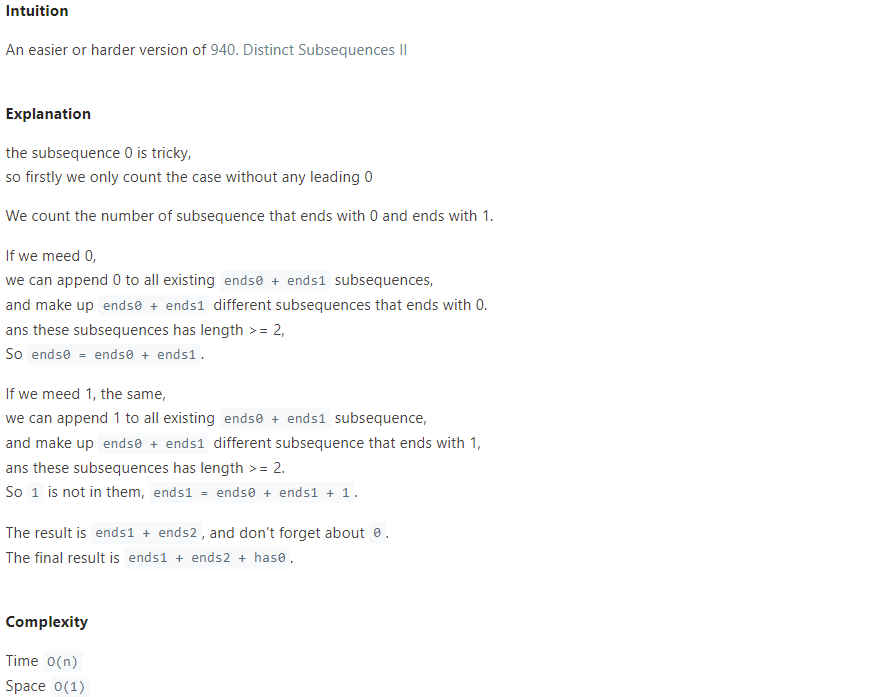
\includegraphics[width=.9\linewidth]{./pic/distinctSubsequence.png}
\begin{minted}[fontsize=\scriptsize,linenos=false]{csharp}
public int numberOfUniqueGoodSubsequences(String binary) {
    int mod = (int)1e9 + 7;
    int endZoo = 0, endOne = 0, hasZoo = 0;
    for (int i = 0; i < binary.length(); i++) 
        if (binary.charAt(i) == '1')
            endOne = (endOne + endZoo + 1) % mod;
        else {
            endZoo = (endZoo + endOne) % mod;
            hasZoo = 1;
        }
    return (endOne + endZoo + hasZoo) % mod;
}
\end{minted}
\begin{itemize}
\item 还有一个没有看懂的
\begin{itemize}
\item \url{https://leetcode-cn.com/problems/number-of-unique-good-subsequences/solution/ju-yi-fan-san-by-avenger-h-34xa/}
\item \url{https://leetcode-cn.com/problems/distinct-subsequences-ii/solution/dong-tai-gui-hua-cong-fen-xi-dao-shi-xian-by-my10y/}
\end{itemize}
\end{itemize}
\begin{minted}[fontsize=\scriptsize,linenos=false]{python}
def numberOfUniqueGoodSubsequences(self, binary: str) -> int:
        M = 10**9+7
        dp = [0]*10
        b = str(int(binary))
        l = len(binary) - len(b)
        if l > 0:
            dp[0] = 1
        for c in b:
            if dp[0] >= 1:
                dp[int(c)] = (sum(dp)) % M
            else:
                dp[int(c)] = ( 1+ sum(dp)) % M
        return sum(dp)%M
\end{minted}
\subsection{714. Best Time to Buy and Sell Stock with Transaction Fee}
\label{sec-1-4-21}
You are given an array prices where prices[i] is the price of a given stock on the ith day, and an integer fee representing a transaction fee.
Find the maximum profit you can achieve. You may complete as many transactions as you like, but you need to pay the transaction fee for each transaction.
Note: You may not engage in multiple transactions simultaneously (i.e., you must sell the stock before you buy again).
\begin{minted}[fontsize=\scriptsize,linenos=false]{csharp}
public int maxProfit(int[] prices, int fee) {
    int n = prices.length;
    int [] sold = new int[n];
    int [] hold = new int[n];
    hold[0] = -prices[0];
    for (int i = 1; i < n; i++) {
        sold[i] = Math.max(sold[i-1], hold[i-1]+prices[i]-fee);
        hold[i] = Math.max(hold[i-1], sold[i-1]-prices[i]);
    }
    return sold[n-1];
}
\end{minted}

\subsection{847. Shortest Path Visiting All Nodes}
\label{sec-1-4-22}
You have an undirected, connected graph of n nodes labeled from 0 to n - 1. You are given an array graph where graph[i] is a list of all the nodes connected with node i by an edge.
Return the length of the shortest path that visits every node. You may start and stop at any node, you may revisit nodes multiple times, and you may reuse edges.
\begin{minted}[fontsize=\scriptsize,linenos=false]{csharp}
public int shortestPathLength(int[][] graph) {
    int n = graph.length;
    int tar = 0, res = 0;
    HashSet<String> s = new HashSet<>();
    Queue<Pair<Integer, Integer>> q = new LinkedList<>();
    for (int i = 0; i < n; i++) {
        int mask = (1 << i);
        tar |= mask;
        s.add(Integer.toString(mask) + "-" + Integer.toString(i));
        q.add(new Pair<>(mask, i));
    }
    while (!q.isEmpty()) {
        for (int i = q.size(); i > 0; i--) {
            Pair cur = q.remove();
            if ((int)cur.getKey() == tar) return res;
            for (int next : graph[(int)cur.getValue()]) {
                int path = (int)cur.getKey() | (1 << next);
                String str = Integer.toString(path) + "-" + Integer.toString(next);
                if (s.contains(str)) continue;
                s.add(str);
                q.add(new Pair<>(path, next));
            }
        }
        ++res;
    }
    return -1;
}
\end{minted}

\subsection{926. Flip String to Monotone Increasing - Medium}
\label{sec-1-4-23}
A binary string is monotone increasing if it consists of some number of 0's (possibly none), followed by some number of 1's (also possibly none).

You are given a binary string s. You can flip s[i] changing it from 0 to 1 or from 1 to 0.

Return the minimum number of flips to make s monotone increasing.
\begin{enumerate}
\item 解题思路与分析:动态规划
\label{sec-1-4-23-1}

这道题给了我们一个只有0和1的字符串,现在说是可以将任意位置的数翻转,即0变为1,或者1变为0,让组成一个单调递增的序列,即0必须都在1的前面,博主刚开始想的策略比较直接,就是使用双指针分别指向开头和结尾,开头的指针先跳过连续的0,末尾的指针向前跳过连续的1,然后在中间的位置分别记录0和1的个数,返回其中较小的那个。这种思路乍看上去没什么问题,但是实际上是有问题的,比如对于这个例子 "10011111110010111011",如果按这种思路的话,就应该将所有的0变为1,从而返回6,但实际上更优的解法是将第一个1变为0,将后4个0变为1即可,最终可以返回5.

这说明了之前的解法是不正确的。这道题可以用动态规划 Dynamic Programming 来做,需要使用两个 dp 数组,其中 cnt1[i] 表示将范围是 [0, i-1] 的子串内最小的将1转为0的个数,从而形成单调字符串。同理,cnt0[j] 表示将范围是 [j, n-1] 的子串内最小的将0转为1的个数,从而形成单调字符串。这样最终在某个位置使得 cnt0[i]+cnt1[i] 最小的时候,就是变为单调串的最优解,这样就可以完美的解决上面的例子,子串 "100" 的最优解是将1变为0,而后面的 "11111110010111011" 的最优解是将4个0变为1,总共加起来就是5,参见代码如下:

\begin{minted}[fontsize=\scriptsize,linenos=false]{csharp}
// 可以用动态规划 Dynamic Programming 来做,需要使用两个 dp 数组,其中 cnt1[i] 表示将范围是 [0, i-1] 的子串内最小的将1转为0的个数,从而形成单调字符串。
// 同理,cnt0[j] 表示将范围是 [j, n-1] 的子串内最小的将0转为1的个数,从而形成单调字符串。
// 这样最终在某个位置使得 cnt0[i]+cnt1[i] 最小的时候,就是变为单调串的最优解,
public int minFlipsMonoIncr(String t) { // bug
    int n = t.length(), ans = Integer.MAX_VALUE;
    char [] s = t.toCharArray();
    int [] l = new int [n+1], r = new int [n+1];
    for (int i = 1, j = n-1; i <= n; i++, --j) {
        l[i] = l[i-1] + (s[i-1] == '0' ? 0 : 1); // cnt left --> right 1--> 0
        r[j] = r[j+1] + (s[j] == '0' ? 1 : 0);
    }
    for (int i = 0; i <= n; i++) 
        ans = Math.min(l[i] + r[i], ans);
    return ans;
}
\end{minted}
\item 解题思路与分析: 空间压缩与简化
\label{sec-1-4-23-2}

我们可以进一步优化一下空间复杂度,用一个变量 cnt1 来记录当前位置时1出现的次数,同时 res 表示使到当前位置的子串变为单调串的翻转次数,用来记录0的个数,因为遇到0就翻1一定可以组成单调串,但不一定是最优解,每次都要和 cnt1 比较以下,若 cnt1 较小,就将 res 更新为 cnt1,此时保证了到当前位置的子串变为单调串的翻转次数最少,并不关心到底是把0变为1,还是1变为0了,其实核心思想跟上面的解法很相近

\begin{minted}[fontsize=\scriptsize,linenos=false]{csharp}
// 用一个变量 cnt1 来记录当前位置时1出现的次数,同时 res 表示使到当前位置的子串变为单调串的翻转次数,
// 用来记录0的个数,因为遇到0就翻1一定可以组成单调串,但不一定是最优解,
// 每次都要和 cnt1 比较以下,若 cnt1 较小,就将 res 更新为 cnt1,
// 此时保证了到当前位置的子串变为单调串的翻转次数最少,并不关心到底是把0变为1,还是1变为0了
public int minFlipsMonoIncr(String t) { // bug
    int n = t.length(), res = 0, cntOne = 0;
    char [] s = t.toCharArray();
    for (int i = 0; i < n; i++) {
        if (s[i] == '0') res++;
        else cntOne++;
        res = Math.min(res, cntOne);
    }
    return res;
}
\end{minted}

早上的时候不是刚写过一个这样的题吗 ? 与1493 的第二种解法有什么区别?
\end{enumerate}

\subsection{1931. Painting a Grid With Three Different Colors}
\label{sec-1-4-24}
You are given two integers m and n. Consider an m x n grid where each cell is initially white. You can paint each cell red, green, or blue. All cells must be painted.
Return the number of ways to color the grid with no two adjacent cells having the same color. Since the answer can be very large, return it modulo 109 + 7.
\begin{itemize}
\item lightweighted轻巧点儿的解题方案: bitmask
\end{itemize}
\begin{minted}[fontsize=\scriptsize,linenos=false]{csharp}
// time O( (2^5) *2 * N)
// SPACE O(N)
//     For m = 5, there are at most 48 valid states for a single column so we can handle it column by column.
//     We encode the color arrangement by bit mask (3 bit for a position) and use dfs to generate the all valid states.
//         Then for each column, we iterator all the states and check if its still valid with the previous column.
public void helper(int m, int pos, HashMap<Integer, Long> dic, int pre, int cur) {
    if (pos == m) {
        dic.put(cur, 1L);
        return;
    }
    //不需要{1, 2, 4} {0, 1, 2} is ok 每个格(实际占用3个bit)
    for (int i = 0; i < 3; i++) {
        if (i == pre) continue; 
        helper(m, pos + 1, dic, i, (cur << 3) | (1 << i)); // 每处理一格,将当前状态左移3位?(实际每个格占用3个bit位)| 现在这个格的值?这个,我好昏呀
    }
}
static int mod = (int) 1e9 + 7;
public int colorTheGrid(int m, int n) {
    HashMap<Integer,Long> dic = new HashMap<>();
    helper(m, 0, dic, -1, 0);     // 这应该就是我想找的精巧不占多少空间的mask了,可是有点儿看不懂
    HashSet<Integer> set = new HashSet<>(dic.keySet());
    for (int i = 1; i < n; i++) { // 动态规划: 用两个图像滚动数组一样轮流记载得出答案
        HashMap<Integer, Long> tmp = new HashMap<>();
        for (int x: set) 
            for (int y : set) 
                if ((x & y) == 0) // 相邻涂色方案为有效方案
                    tmp.put(y, (tmp.getOrDefault(y, 0L) + dic.get(x)) % mod);
        dic = tmp;
    }
    long res = 0L;
    for (Long x : dic.values()) {
        res += x;
        res %= mod;
    }
    return (int) res;
}
\end{minted}
\begin{itemize}
\item 比较传统一点儿的解法,思路清晰
\end{itemize}
\begin{minted}[fontsize=\scriptsize,linenos=false]{csharp}
// 参考的答案里,这个最逻辑简单、通俗大众易懂,但稍显笨重,两个图,用一个链表来记忆一行的涂色方案,如果有更精巧一点儿的bitmask,是我想找的答案
// https://leetcode.com/problems/painting-a-grid-with-three-different-colors/discuss/1334366/Easy-Java-comments-28ms-O(n*P*P)-complexity-memory-O(P)-where-P-is-column-permutations-count 这个又稍嫌太偏了,考得极少,不易懂,容易出错,可是bitmask又只能set 1 or 0,BitSet()可以吗?
// 先预处理得到单行的所有有效涂色方案,
// 再进一步计算得到每种单行方案对应的有效邻行方案
// 在此基础上,结合动态规划方法,逐行求解各种涂色状态对应的方案总数,最后统计得到总方案数。
public int colorTheGrid(int m, int n) {
// 获得单行所有涂色方案
    Map<Integer, List<Integer>> line = new HashMap<>(); //  3^m ways of paying one row
    int range = (int)Math.pow(3, m); // 用0、1、2表示各个网格的颜色,key为方案对应的数值,value为方案对应的数组
    for (int i = 0; i < range; i++) {
        List<Integer> list = new ArrayList<>(); //  val val values (0, 1, 2) of every m cols into list
        int val = i;
        for (int j = 0; j < m; j++) {
            list.add(val % 3);
            val /= 3;
        }
        boolean valid = true; // 确认该数组中是否存在相邻位置颜色相同
        for (int j = 1; j < m; j++) 
            if (list.get(j-1) == list.get(j)) {
                valid = false;
                break;
            }
        if (valid) line.put(i, list); // 相邻网格颜色均不同,为有效方案,加入哈希表
    }
// 预处理得到每种单行方案对应的有效邻行方案
    Map<Integer, List<Integer>> adj = new HashMap<>();
    Iterator it = line.entrySet().iterator();
    while (it.hasNext()) {     //  3^m ways of paying one row
        Map.Entry entry = (Map.Entry)it.next();
        int va = (int)entry.getKey();
        List<Integer> lva = (List<Integer>)entry.getValue();
        adj.put(va, new ArrayList<Integer>());
        Iterator itb = line.entrySet().iterator();
        while (itb.hasNext()) { //  3^m ways of paying one row
            Map.Entry enb = (Map.Entry)itb.next(); 
            int vb = (int)enb.getKey();
            List<Integer> lvb = (List<Integer>)enb.getValue();
            boolean valid = true;
            for (int i = 0; i < m; i++) 
                if (lva.get(i) == lvb.get(i)) {
                    valid = false;
                    break;
                } // among 3^m ways of painting one row, how many is valid, and valid mask into adj.get(va);
            if (valid) adj.get(va).add(vb); 
        }
    }
// 动态规划,逐行求解方案数
    int mod = (int)(1e9+7);
    long [] dp = new long [range];  // 上一行各种涂色方案对应的总方法数
    for (int i = 0; i < range; i++) // 初始化
        dp[i] = line.containsKey(i) ? 1 : 0;
    for (int i = 1; i < n; i++) {   // 从第二行开始动态规划
        long [] cur = new long [range];  // 新一行各种涂色方案对应的总方法数
        for (int j = 0; j < range; j++) 
            if (adj.containsKey(j)) {    // 该方案有效
                for (int v : adj.get(j)) // 遍历有效的相邻方案
                    cur[j] = (cur[j] + dp[v]) % mod; // 总方法数累加
            }
        System.arraycopy(cur, 0, dp, 0, range);
    }
    long ans = 0;
    for (int i = 0; i < range; i++) 
        ans = (ans + dp[i]) % mod;
    return (int)ans;
}
\end{minted}

\subsection{313. Super Ugly Number}
\label{sec-1-4-25}
A super ugly number is a positive integer whose prime factors are in the array primes.
Given an integer n and an array of integers primes, return the nth super ugly number.
The nth super ugly number is guaranteed to fit in a 32-bit signed integer.
\begin{minted}[fontsize=\scriptsize,linenos=false]{csharp}
static class Node implements Comparable<Node> {
    private int index;
    private int val;
    private int prime;
    public Node(int index, int val, int prime) {
        this.index = index;
        this.val = val;
        this.prime = prime;
    }
    public int compareTo(Node other) {
        return this.val - other.val;
    }
}
public int nthSuperUglyNumber(int n, int[] primes) {
    final int [] arr = new int[n];
    arr[0] = 1;              // 1 is the first ugly number
    final Queue<Node> q = new PriorityQueue<>();
    for (int i = 0; i < primes.length; ++i) 
        q.add(new Node(0, primes[i], primes[i]));
    for (int i = 1; i < n; ++i) {
        Node node = q.peek(); // get the min element and add to arr
        arr[i] = node.val;
        do {             // update top elements
            node = q.poll();
            node.val = arr[++node.index] * node.prime;
            q.add(node); // push it back
        } while (!q.isEmpty() && q.peek().val == arr[i]); // prevent duplicate
    }
    return arr[n - 1];
}
\end{minted}
\begin{itemize}
\item 下面这种解法也很巧妙
\end{itemize}
\begin{minted}[fontsize=\scriptsize,linenos=false]{csharp}
public int nthSuperUglyNumber(int n, int[] primes) {
    int m = primes.length;
    int [] ans = new int[n]; // 存放1-n个SuperUglyNumber
    ans[0] = 1;              // 第一个SuperUglyNumber是1
    int [] next = new int[m];
    for (int i=0; i < m; i++)
        next[i] = 0;         // 初始化
    int cnt = 1, min = Integer.MAX_VALUE, tmp = 0;
    while (cnt < n) {
        min = Integer.MAX_VALUE;
        for (int i = 0; i < m; i++){
             tmp = ans[next[i]] * primes[i];
             min = Math.min(min, tmp);
        }
        for (int i = 0; i < m; i++)
            if (min == ans[next[i]] * primes[i])
                next[i]++;
        ans[cnt++] = min;			
    }
    return ans[n-1];		
}
\end{minted}

\subsection{backpack III}
\label{sec-1-4-26}
\begin{minted}[fontsize=\scriptsize,linenos=false]{csharp}
public int backPackIII(int[] A, int[] V, int m) {
    int n = A.length;
    int [] dp = new int[m+1];
    for (int i = 1; i <= m; i++) {
        for (int j = 0; j < n; j++) {
            if (i - A[j] >= 0)
                dp[i] = Math.max(dp[i], dp[i-A[j]] + V[j]);
        }
    }
    return dp[m];
}
\end{minted}

\subsection{879. Profitable Schemes - Hard 0-1背包问题}
\label{sec-1-4-27}
There is a group of n members, and a list of various crimes they could commit. The ith crime generates a profit[i] and requires group[i] members to participate in it. If a member participates in one crime, that member can't participate in another crime.

Let's call a profitable scheme any subset of these crimes that generates at least minProfit profit, and the total number of members participating in that subset of crimes is at most n.

Return the number of schemes that can be chosen. Since the answer may be very large, return it modulo 109 + 7.
\begin{enumerate}
\item 解题思路与分析: DP
\label{sec-1-4-27-0-1}

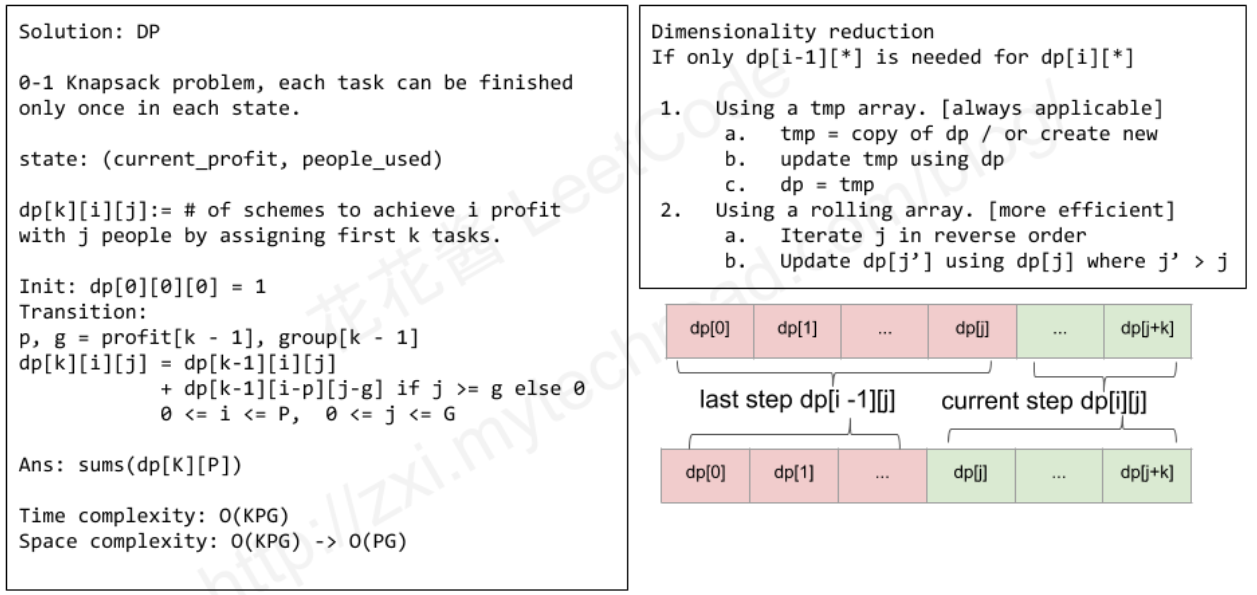
\includegraphics[width=.9\linewidth]{./pic/crime.png}

\begin{itemize}
\item 题目中说了结果可能非常大,要对一个超大数取余,看到这里,我们也就该明白为了不爆栈,只能用动态规划 Dynamic Programming 来做,LeetCode 里有好多题都是要对这个 1e9+7 取余,不知道为啥都是对这个数取余。Anyway,who cares,还是来想想 dp 数组如何定义以及怎么推导状态转移方程吧。
\end{itemize}

首先来看分配黑帮资源时候都需要考虑哪些因素,总共有三点,要干几票买卖,要用多少人,能挣多少钱。所以我们需要一个三维的 dp 数组,其中 dp[k][i][j] 表示最多干k票买卖,总共用了i个人,获得利润为j的情况下分配方案的总数,初始化 dp\footnotemark[1]{}\textsuperscript{,}\,\footnotemark[1]{}\textsuperscript{,}\,\footnotemark[1]{} 为1。

现在来推导状态转移方程,整个规划的核心是买卖,总共买卖的个数是固定的,每多干一票买卖,可能的分配方法就可能增加,但不可能减少的,因为假如当前已经算出来做 k-1 次买卖的分配方法总数,再做一次买卖,之前的分配方法不会减少,顶多是人数不够,做不成当前这票买卖而已,所以我们的 dp[k][i][j] 可以先更新为 dp[k-1][i][j],然后再来看这第k个买卖还能不能做,我们知道假设这第k个买卖需要g个人,能获得利润p,只有当我们现在的人数i大于等于g的时候,才有可能做这个任务,我们要用g个人来做任务k的话,那么其余的 k-1 个任务只能由 i-g 个人来做了,而且由于整个需要产生利润j,第k个任务能产生利润p,所以其余的 k-1 个任务需要产生利润 j-p,由于利润不能是负值,所以我们还需要跟0比较,取二者的最大值

综上所述,若我们选择做任务k,则能新产生的分配方案的个数为 dp[k-1][i-g][max(0,j-p)],记得每次累加完要对超大数取余。最终我们需要将 dp[n][i][P] ( 0 <= i <= G ) 累加起来,因为我们不一定要全部使用G个人,只要能产生P的利润,用几个人都没关系,而k是表示最多干的买卖数,可能上并没有干到这么多,所以只需要累加人数这个维度即可,

\begin{minted}[fontsize=\scriptsize,linenos=false]{csharp}
static final int mod = (int)1e9 + 7;
public int profitableSchemes(int n, int minProfit, int[] group, int[] profit) {
    int m = group.length, ans = 0;
    int [][][] dp = new int [m+1][n+1][minProfit+1];
    dp[0][0][0] = 1;
    for (int i = 1; i <= m; i++) {   // 遍历每桩案件
        int g = group[i-1], p = profit[i-1];
        for (int j = 0; j <= n; j++) // 遍历人数
            for (int k = 0; k <= minProfit; k++) {
                dp[i][j][k] = dp[i-1][j][k];
                if (j >= g)   // 在本桩案件人手够用的前提下,办与不办此案的方案数相加
                    dp[i][j][k] = (dp[i][j][k] + dp[i-1][j-g][Math.max(0, k-p)]) % mod;
            }
    }
    for (int i = 0; i <= n; i++) 
        ans = (ans + dp[m][i][minProfit]) % mod;
    return ans;
}
\end{minted}
\item 优化一下空间复杂度: 二维dp Dimension reduction by using rolling array.
\label{sec-1-4-27-1}

因为当前做的第k个任务,只跟前 k-1 个任务的分配方案有关,所以并不需要保存所有的任务个数的分配方式。这样我们就节省了一个维度,但是需要注意的是,更新的时候i和j只能从大到小更新,这个其实也不难理解,因为此时 dp[i][j] 存的是前 k-1 个任务的分配方式,所以更新第k个任务的时候,一定要从后面开始覆盖,因为用到了前面的值,若从前面的值开始更新的话,就不能保证用到的都是前 k-1 个任务的分配方式,有可能用到的是已经更新过的值,就会出错.
\begin{minted}[fontsize=\scriptsize,linenos=false]{csharp}
static final int mod = (int)1e9 + 7;
public int profitableSchemes(int n, int minProfit, int[] group, int[] profit) {
    int m = group.length, ans = 0;
    int [][] dp = new int [n+1][minProfit+1];
    dp[0][0] = 1;
    for (int i = 1; i <= m; i++) {   // 遍历每桩案件
        int g = group[i-1], p = profit[i-1];
        for (int j = n; j >= g; j--)  // 当压缩了一维空间,从后往前遍历以免产生赃数据
            for (int k = minProfit; k >= 0; k--) 
                dp[j][k] = (dp[j][k] + dp[j-g][Math.max(0, k-p)]) % mod;
    }
    for (int i = 0; i <= n; i++) 
        ans = (ans + dp[i][minProfit]) % mod;
    return ans;
}
\end{minted}
\item 递归dfs + 记忆数组
\label{sec-1-4-27-2}

基本思想跟解法一没有太大的区别,递归的记忆数组其实跟迭代形式的 dp 数组没有太大的区别,作用都是保存中间状态从而减少大量的重复计算。这里稍稍需要注意下的就是递归函数中的 corner case,当 k=0 时,则根据j的值来返回0或1,当j小于等于0,返回1,否则返回0,相当于修改了初始化值(之前都初始化为了整型最小值),然后当j小于0时,则j赋值为0,因为利润不能为负值。然后就看若当前的 memo[k][i][j] 已经计算过了,则直接返回即可
\begin{minted}[fontsize=\scriptsize,linenos=false]{csharp}
public int profitableSchemes(int n, int minProfit, int[] group, int[] profit) {
    m = group.length;
    this.n = n;
    this.minProfit = minProfit;
    dp = new int [m+1][n+1][minProfit+1];
    for (int i = 0; i <= m; i++) 
        for (int j = 0; j <= n; j++) 
            Arrays.fill(dp[i][j], Integer.MIN_VALUE);
    return dfs(m, n, minProfit, group, profit);
}
static final int mod = (int)1e9 + 7;
int m, n, minProfit;
int [][][] dp;
private int dfs(int i, int j, int k, int [] group, int [] profit) {
    if (i == 0) return k <= 0 ? 1 : 0;
    if (k < 0) k = 0;
    if (dp[i][j][k] != Integer.MIN_VALUE) return dp[i][j][k];
    int g = group[i-1], p = profit[i-1];
    int ans = dfs(i-1, j, k, group, profit);
    if (j >= g)
        ans = (ans + dfs(i-1, j-g, Math.max(0, k-p), group, profit)) % mod;
    return dp[i][j][k] = ans;
}
\end{minted}
\end{enumerate}

\subsection{377. Combination Sum IV 没能认出这个题目是考DP}
\label{sec-1-4-28}
Given an array of distinct integers nums and a target integer target, return the number of possible combinations that add up to target.
The answer is guaranteed to fit in a 32-bit integer.
\begin{enumerate}
\item 解题思路与分析: dfs记忆化搜索
\label{sec-1-4-28-1}

思路: 一开始想到用DFS来做, 但是有个问题就是这种方式得到的答案各个数字排列是无序的, 也就是1, 3和3, 1这种只是一个答案, 

\begin{minted}[fontsize=\scriptsize,linenos=false]{csharp}
public int combinationSum4(int[] a, int target) { // 带记忆化的来搜索,用数组还是用图,可能也看数据规模吧
    return helper(a, target);
}
Map<Integer, Integer> dp = new HashMap<>();
private int helper(int[] a, int target) {
    if (target < 0) return 0;
    if (target == 0) return 1;
    if (dp.containsKey(target)) return dp.get(target);
    int ans = 0;
    for (int i = 0; i < a.length; i++) 
        ans += helper(a, target-a[i]);
    dp.put(target, ans);
    return ans;
}
\end{minted}
\item 解题思路与分析: DP
\label{sec-1-4-28-2}

然后又想把数字保存起来, 在得到一个答案的时候对这些数字再求一次总共排列的个数, 这种方式还有问题就是在求总排列个数的时候比如2, 1, 1三个加一起等于4, 总的排列个数即为(3!/2!), 但是当数字个数很多的时候阶乘太大, 根本无法计算.

然后就想到可以用动态规划来做, 也是一个背包问题, 求出[1, target]之间每个位置有多少种排列方式, 这样将问题分化为子问题. 状态转移方程可以得到为: 

dp[i] = sum(dp[i - nums[j]]),  (i-nums[j] > 0);

如果允许有负数的话就必须要限制每个数能用的次数了, 不然的话就会得到无限大的排列方式, 比如1, -1, target = 1;

\begin{minted}[fontsize=\scriptsize,linenos=false]{csharp}
public int combinationSum4(int[] nums, int target) {
    int n = nums.length;
    int [] dp = new int [target +1 ];
    dp [0] = 1;
    for (int i = 1; i <= target; i++) {
        for (int j = 0; j < n; j++) {
            if (i - nums[j] >= 0)
                dp[i] += dp[i-nums[j]];
        }
    }
    return dp[target];
}
\end{minted}

\begin{itemize}
\item 针对适当情况的优化:如果 target 远大于 nums 数组的个数的话,上面的算法可以做适当的优化,先给 nums 数组排个序,然后从1遍历到 target,对于i小于数组中的数字x时,直接 break 掉,因为后面的数更大,其余地方不变
\begin{minted}[fontsize=\scriptsize,linenos=false]{csharp}
public int combinationSum4(int[] a, int target) { // if target 远大于 数组元素个数
    int n = a.length;
    Arrays.sort(a);
    int [] dp = new int [target + 1];
    dp[0] = 1;
    for (int i = 1; i <= target; i++)
        for (Integer v : a) {
            if (i < v) break;
            dp[i] += dp[i-v];
        }
    return dp[target];
}
\end{minted}
\end{itemize}
\end{enumerate}


\subsection{1049. Last Stone Weight II}
\label{sec-1-4-29}
You are given an array of integers stones where stones[i] is the weight of the ith stone.
We are playing a game with the stones. On each turn, we choose any two stones and smash them together. Suppose the stones have weights x and y with x <= y. The result of this smash is:
If x \texttt{= y, both stones are destroyed, and
If x !} y, the stone of weight x is destroyed, and the stone of weight y has new weight y - x.
At the end of the game, there is at most one stone left.
Return the smallest possible weight of the left stone. If there are no stones left, return 0.
\begin{minted}[fontsize=\scriptsize,linenos=false]{csharp}
public int lastStoneWeightII(int[] stones) {
    int n = stones.length;
    int sum = Arrays.stream(stones).sum();
    boolean[] dp = new boolean[sum+1];
    dp[0] = true;
    sum = 0;
    for (int v : stones) {
        sum += v;
        for (int i = sum; i >= v; i--) 
            if (dp[i-v]) dp[i] = true;
    }
    for (int i = sum/2; i >= 0; i--) 
        if (dp[i]) return sum - i * 2;
    return 0;
}
\end{minted}

\subsection{810. Chalkboard XOR Game - Hard}
\label{sec-1-4-30}
You are given an array of integers nums represents the numbers written on a chalkboard.

Alice and Bob take turns erasing exactly one number from the chalkboard, with Alice starting first. If erasing a number causes the bitwise XOR of all the elements of the chalkboard to become 0, then that player loses. The bitwise XOR of one element is that element itself, and the bitwise XOR of no elements is 0.

Also, if any player starts their turn with the bitwise XOR of all the elements of the chalkboard equal to 0, then that player wins.

Return true if and only if Alice wins the game, assuming both players play optimally.
There are three cases to consider:
\begin{minted}[fontsize=\scriptsize,linenos=false]{csharp}
Case 1- At the beginning of the game, XOR of all the elements are 0, then Alice wins before the game starts.

Case 2 - XOR!=0 and nums.length is even:
Let’s try to use proof by contradiction. S=(x1^x2…^xn)
Assume s!=0, let’s try to find contradiction
XOR s to both sides
s^s=s^(x1^x2…^xn)
s^s=0 => 0= s^(x1^x2…^xn)
0=(s^x1)^(s^x2)…^(s^xn)
Now let’s factor s from each bracket
0=(s^s…^s)^(x1^x2…^xn)
Since the number of x1..xn is even, the number of s in the left bracket is even, each number ^ itself even times results to 0.
0=0^(x1^x2…^xn)
0^ any number is itself so
0=(x1^x2…^xn)=s => 0=s
You see that there is a contradiction (compare with initial assumption s!=0), at the beginning we assumed s!=0
Then our assumption is wrong. So, s==0 then Alice wins

Case 3- XOR!=0 and nums.length is odd:
Let’s try to use proof by contradiction here like the other case
Assume s!=0, let’s try to find contradiction
XOR s to both sides
s^s=s^(x1^x2…^xn)
s^s=0 => 0= s^(x1^x2…^xn)
0=(s^x1)^(s^x2)…^(s^xn)
Now let’s factor s from each bracket
0=(s^s…^s)^(x1^x2…^xn)
Since the number of x1..xn is odd, the number of s in the left bracket is odd, each number ^ itself odd times results to itself.
0=s^(x1^x2…^xn) => 0=s^s
Any number XOR itself becomes zero
0=s^s=0
You see here we couldn’t find the contradiction
\end{minted}

\begin{minted}[fontsize=\scriptsize,linenos=false]{csharp}
public boolean xorGame(int[] nums) {
    int xor = 0 ;
    for (int i : nums) 
        xor = xor ^ i ;
    if (xor == 0 || (nums.length & 1) == 0)
        return true ;
    return false ;
}
\end{minted}
\begin{itemize}
\item 硬瓣出来的: 注意同猫老鼠游戏2一样,要回的是某一方赢与否,与1有点儿区别.
\end{itemize}
\begin{minted}[fontsize=\scriptsize,linenos=false]{csharp}
private boolean helper(int [] arr, int i, int xor) { // xor: the current leftover array xor result
    if (i == n) return (i % 2 == 0);
    if (dp[i] != null) return dp[i];
    if (xor == 0) return (i % 2 == 0); // to be noted
    int tmp = 0;
    if (i % 2 == 0) { // alice's turn
        for (int j = 0; j < n; j++) {
            if (arr[j] == -1) continue;
            if ((arr[j] ^ xor) == 0) continue;
            tmp = arr[j];
            arr[j] = -1;
            if (helper(arr, i+1, xor^tmp)) return dp[i] = true;
            arr[j] = tmp;
        }
        return dp[i] = false;
    } else { // bob's turn
        for (int j = 0; j < n; j++) {
            if (arr[j] == -1) continue;
            if ((arr[j] ^ xor) == 0) continue;
            tmp = arr[j];
            arr[j] = -1;
            if (!helper(arr, i+1, xor^tmp)) return dp[i] = false;
            arr[j]= tmp;
        }
        return dp[i] = true;
    }
}
Boolean [] dp; // alice win states
int n;
public boolean xorGame(int[] arr) {
    n = arr.length;
    dp = new Boolean [n];
    int [] xor = new int [n];
    for (int i = 0; i < n; i++) 
        xor[i] = (i == 0 ? 0 : xor[i-1]) ^ arr[i];
    return helper(arr, 0, xor[n-1]); // i: turn
}
\end{minted}

\subsection{1449. Form Largest Integer With Digits That Add up to Target}
\label{sec-1-4-31}
Given an array of integers cost and an integer target. Return the maximum integer you can paint under the following rules:
The cost of painting a digit (i+1) is given by cost[i] (0 indexed).
The total cost used must be equal to target.
Integer does not have digits 0.
Since the answer may be too large, return it as string.
If there is no way to paint any integer given the condition, return "0".
\begin{minted}[fontsize=\scriptsize,linenos=false]{csharp}
public String largestNumber(int[] cost, int target) { 
    int n = cost.length;
    int [] dp = new int [target+1];
    Arrays.fill(dp, -1);
    dp[0] = 0;
    for (int i = 0; i < n; i++) {
        for (int j = cost[i]; j <= target; j++) {
            if (dp[j-cost[i]] >= 0)
                dp[j] = Math.max(dp[j], dp[j-cost[i]]+1);
        }
    }
    if (dp[target] < 0) return "0";
    char [] ans = new char[dp[target]]; // 采樱桃机器人数组路线那天可以想出来,今天这个路径居然没有想出来!
    int left = target;
    for (int i = 0; i < dp[target]; i++) {
        for (int j = n; j > 0; j--) {
            if (left >= cost[j-1] && dp[left] == dp[left-cost[j-1]] + 1) {
                ans[i] = (char)('0' + j);
                left -= cost[j-1];
                break;
            }
        }
    }
    return String.valueOf(ans);
}
\end{minted}

\subsection{516. Longest Palindromic Subsequence}
\label{sec-1-4-32}
Given a string s, find the longest palindromic subsequence's length in s.
A subsequence is a sequence that can be derived from another sequence by deleting some or no elements without changing the order of the remaining elements.
\begin{minted}[fontsize=\scriptsize,linenos=false]{csharp}
 public int longestPalindromeSubseq(String s) {
    int n = s.length();
    int [][] dp = new int [n][n];
    dp[n-1][n-1] = 1;
    for (int i = n-2; i >= 0; i--) {
        dp[i][i] = 1;
        for (int j = i+1; j < n; j++) {
            if (s.charAt(i) == s.charAt(j))
                dp[i][j] = 2 + dp[i+1][j-1];
            else dp[i][j] = Math.max(dp[i+1][j], dp[i][j-1]);
        }
    }
    return dp[0][n-1];
}
\end{minted}

\subsection{1143. Longest Common Subsequence}
\label{sec-1-4-33}
Given two strings text1 and text2, return the length of their longest common subsequence. If there is no common subsequence, return 0.
A subsequence of a string is a new string generated from the original string with some characters (can be none) deleted without changing the relative order of the remaining characters.
For example, "ace" is a subsequence of "abcde".
A common subsequence of two strings is a subsequence that is common to both strings.
\begin{minted}[fontsize=\scriptsize,linenos=false]{csharp}
public int longestCommonSubsequence(String S, String T) {
    int m = S.length();
    int n = T.length();
    int [][] dp = new int [m+1][n+1];
    for (int i = 1; i <= m; i++) 
        for (int j = 1; j <= n; j++) 
            if (S.charAt(i-1) == T.charAt(j-1)) dp[i][j] = dp[i-1][j-1] + 1;
            else dp[i][j] = Math.max(dp[i-1][j], dp[i][j-1]);
    return dp[m][n];
}
\end{minted}

\subsection{1092. Shortest Common Supersequence - Hard}
\label{sec-1-4-34}
Given two strings str1 and str2, return the shortest string that has both str1 and str2 as subsequences. If there are multiple valid strings, return any of them.

A string s is a subsequence of string t if deleting some number of characters from t (possibly 0) results in the string s.
\begin{itemize}
\item 参考的标准答案:
\end{itemize}
\begin{minted}[fontsize=\scriptsize,linenos=false]{csharp}
public void longestCommonSubsequence(String S, String T) { // 标准模板,记住
    int m = S.length();
    int n = T.length();
    for (int i = 1; i <= m; i++) 
        for (int j = 1; j <= n; j++) 
            if (S.charAt(i-1) == T.charAt(j-1)) dp[i][j] = dp[i-1][j-1] + 1;
            else dp[i][j] = Math.max(dp[i-1][j], dp[i][j-1]);
}
int [][] dp;
public String shortestCommonSupersequence(String s, String t) {
    int m = s.length();
    int n = t.length();
    dp = new int [m+1][n+1];
    longestCommonSubsequence(s, t); // fill dp table
    int i = m, j = n;
    StringBuilder sb = new StringBuilder();
    while (i-1 >= 0 && j-1 >= 0) {
        if (s.charAt(i-1) == t.charAt(j-1)) {
            sb.append(s.charAt(i-1));
            --i;
            --j;
        } else {
            if (dp[i][j] == dp[i-1][j]) {
                sb.append(s.charAt(i-1));
                --i;
            } else {
                sb.append(t.charAt(j-1));
                --j;
            }
        }
    }
    if (i > 0) sb.append((new StringBuilder(s.substring(0, i))).reverse());
    if (j > 0) sb.append((new StringBuilder(t.substring(0, j))).reverse());
    return sb.reverse().toString();
}
\end{minted}
\begin{itemize}
\item 自己写的
\end{itemize}
\begin{minted}[fontsize=\scriptsize,linenos=false]{csharp}
public String getLongestCommonSubsequence(String S, String T) { // 标准模板,记住
    int m = S.length();
    int n = T.length();
    int [][] dp = new int [m+1][n+1];
    for (int i = 1; i <= m; i++) 
        for (int j = 1; j <= n; j++) 
            if (S.charAt(i-1) == T.charAt(j-1)) dp[i][j] = dp[i-1][j-1] + 1;
            else dp[i][j] = Math.max(dp[i-1][j], dp[i][j-1]);
    int i = m, j = n;
    StringBuilder sb = new StringBuilder();
    while (i-1 >= 0 && j-1 >= 0) {
        if (S.charAt(i-1) == T.charAt(j-1)) {
            sb.insert(0, S.charAt(i-1));
            --i;
            --j;
        } else {
            if (dp[i-1][j] >= dp[i][j-1]) --i;
            else --j;
        }
    }
    return sb.toString();
}
public String shortestCommonSupersequence(String s, String t) {
    int m = s.length();
    int n = t.length();
    int i = 0, j = 0;
    String sub = getLongestCommonSubsequence(s, t);
    String res = "";
    for (char c : sub.toCharArray()) {
        while (s.charAt(i) != c) {
            res += s.charAt(i);
            i++;
        }
        while (t.charAt(j) != c) {
            res += t.charAt(j);
            j++;
        }
        res += c;
        i++;
        j++;
    }
    return res + s.substring(i) + t.substring(j);
}
\end{minted}
\subsection{546. Remove Boxes - Hard}
\label{sec-1-4-35}
You are given several boxes with different colors represented by different positive numbers.

You may experience several rounds to remove boxes until there is no box left. Each time you can choose some continuous boxes with the same color (i.e., composed of k boxes, k >= 1), remove them and get k * k points.

Return the maximum points you can get.
\begin{minted}[fontsize=\scriptsize,linenos=false]{csharp}
// 定义dp[l][r][k]表示在[l, r]区间并且在后面包含了k个与boxes[r]相同颜色的boxes的情况下,可以获得的最大得分,显然题目要求的就是dp[0][boxes.size() - 1][0]。
// 首先将dp[l][r][k]的值初始化为dp[l][r - 1][0] + (k + 1)^2,表示首先消除l到r-1之间的boxes,然后将boxes[r]连同后面的k个boxes一起消除。
// 然后就尝试对dp[l][r][k]进行更新了:
// 如果在l到r-1区间内有boxes[i]和boxes[r]相同的字符,那么可以尝试首先将区间[i + 1, r - 1]消除,这样i就和后面的k + 1个boxes连起来了,
// 其可以获得分数就是需要进一步计算的dp[l][i][k + 1]。
private int dfs(int [] arr, int i, int j, int  k) {
    if (i > j) return 0;
    if (dp[i][j][k] > 0) return dp[i][j][k];
    int res = dfs(arr, i, j-1, 0) + (k+1)*(k+1);
    for (int x = i; x < j; x++) 
        if (arr[x] == arr[j]) {
            res = Math.max(res, dfs(arr, i, x, k+1) + dfs(arr, x+1, j-1, 0));
        }
    return dp[i][j][k] = res;
}
int [][][] dp;
int n;
public int removeBoxes(int[] boxes) {
    n = boxes.length;
    dp = new int [n][n][n];
    return dfs(boxes, 0, n-1, 0);
}
\end{minted}
\subsection{1531. String Compression II - Hard}
\label{sec-1-4-36}
Run-length encoding is a string compression method that works by replacing consecutive identical characters (repeated 2 or more times) with the concatenation of the character and the number marking the count of the characters (length of the run). For example, to compress the string "aabccc" we replace "aa" by "a2" and replace "ccc" by "c3". Thus the compressed string becomes "a2bc3".

Notice that in this problem, we are not adding '1' after single characters.

Given a string s and an integer k. You need to delete at most k characters from s such that the run-length encoded version of s has minimum length.

Find the minimum length of the run-length encoded version of s after deleting at most k characters.
\begin{minted}[fontsize=\scriptsize,linenos=false]{csharp}
public int getLengthOfOptimalCompression(String t, int k) {
    n = t.length();
    s = t.toCharArray();
    dp = new Integer [n][n-k+1]; // int [n][n-k+1] 而不是 [n][k+1] 
    return dfs(0, n-k);
}
Integer [][] dp;
char [] s;
int n;
private int dfs(int idx, int k) { // 求从下标 i 开始向后,所有长度为 k 的子序列中,编码后的最小长度
    if (k == 0) return 0;         // 当下标越界时还未找到长度为 k 的子序列
    if (idx == n) return Integer.MAX_VALUE;
    if (dp[idx][k] != null) return dp[idx][k];
    int ans = Integer.MAX_VALUE, cnt = 0;
    boolean [] vis = new boolean [26];
    for (int i = idx; i < n; i++) {
        if (vis[s[i]-'a']) continue; // 优化:当前字母是已处理过的字母, 遍历26个字母的可能性,重复的跳过
        if (idx > 0 && s[i] == s[idx-1]) continue; // 另一种重复的处理
        cnt = 0;
        for (int j = i; j < n; j++) {
            if (s[j] != s[i]) continue;
            cnt++; // 数左半片段中,与s[i]相同的字母的个数
            if (k - cnt < 0) break; // 如果左半部分长度大于子序列长度,退出
            int rite = dfs(j+1, k-cnt);
            if (rite == Integer.MAX_VALUE) continue; 
            int left = ("" + cnt).length();
            ans = Math.min(ans, left + rite + (left == 1 && cnt == 1 ? 0 : 1));
        }
    }
    return dp[idx][k] = ans;
}
\end{minted}
\begin{enumerate}
\item 解题思路与分析: 动态规划
\label{sec-1-4-36-1}
\begin{minted}[fontsize=\scriptsize,linenos=false]{csharp}
public int getLengthOfOptimalCompression(String s, int k) { // 与上面的思路差不多,这里自顶向下,上面的dfs自底向上
    int n = s.length();
    int [][] f = new int[n+1][k+1];
    for (int i = 0; i <= n; i++) 
        Arrays.fill(f[i], Integer.MAX_VALUE >> 1);
    f[0][0] = 0;
    for (int i = 1; i <= n; ++i) 
        for (int j = 0; j <= k && j <= i; ++j) {
            if (j > 0) // 先初始化为删除当前字符为删除的第j个字符的情况
                f[i][j] = f[i - 1][j - 1];
            int same = 0, diff = 0;
            for (int x = i; x >= 1 && diff <= j; x--) {
                if (s.charAt(x-1) == s.charAt(i-1)) {
                    same++; // 数与当前字符连续相同的字符的个数
                    f[i][j] = Math.min(f[i][j], f[x-1][j - diff] + calc(same));
                } else diff++;
            }
        }
    return f[n][k];
}
public int calc(int x) {
    if (x == 1) return 1;
    if (x < 10) return 2;
    if (x < 100) return 3;
    return 4;
}
\end{minted}
\item 决策类DP总结
\label{sec-1-4-36-2}
\begin{itemize}
\item \url{https://leetcode-cn.com/problems/string-compression-ii/solution/jie-ti-si-kao-guo-cheng-yu-jie-fa-zong-jie-by-ruit/}
\end{itemize}
\end{enumerate}

\subsection{1039. Minimum Score Triangulation of Polygon}
\label{sec-1-4-37}
You have a convex n-sided polygon where each vertex has an integer value. You are given an integer array values where values[i] is the value of the ith vertex (i.e., clockwise order).
You will triangulate the polygon into n - 2 triangles. For each triangle, the value of that triangle is the product of the values of its vertices, and the total score of the triangulation is the sum of these values over all n - 2 triangles in the triangulation.
Return the smallest possible total score that you can achieve with some triangulation of the polygon.
\begin{minted}[fontsize=\scriptsize,linenos=false]{csharp}
// 动态规划,递归可以使逻辑简单(本质还是动态规划)将多边形起
// 始位置设为start,end, 用一个数组dp来记录任意起始位置的score
// 为了计算dp[start][end], 我们用一个index k在start到end之间遍
// 历dp[start][end] = min(dp[start][k] + dp[k][end] + A[start]
// * A[k] * A[end])结果为dp[0][n - 1]注意:相邻的dp[i][i + 1]
// = 0, 因为两条边无法组成三角形
private int dfs(int [] arr, int x, int y) {
    if (y - x < 2) return dp[x][y] = 0;
    if (dp[x][y] > 0) return dp[x][y];
    int min = Integer.MAX_VALUE;
    for (int i = x+1; i < y; i++) 
        min = Math.min(min, dfs(arr, x,  i) + dfs(arr, i, y) + arr[x]*arr[i]*arr[y]);
    return dp[x][y] = min;
}
int [][] dp;
int n;
public int minScoreTriangulation(int[] arr) {
    n = arr.length;
    dp = new int [n][n];
    return dfs(arr, 0, n-1);
}
\end{minted}

\subsection{375. Guess Number Higher or Lower II - Medium}
\label{sec-1-4-38}
We are playing the Guessing Game. The game will work as follows:

I pick a number between 1 and n.

You guess a number.

If you guess the right number, you win the game.

If you guess the wrong number, then I will tell you whether the number I picked is higher or lower, and you will continue guessing.

Every time you guess a wrong number x, you will pay x dollars. If you run out of money, you lose the game.

Given a particular n, return the minimum amount of money you need to guarantee a win regardless of what number I pick.

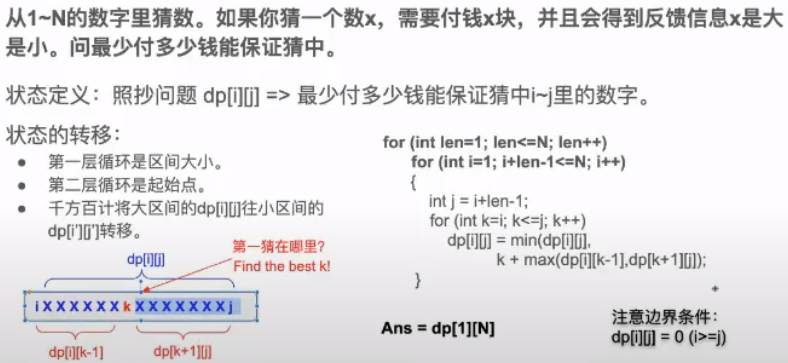
\includegraphics[width=.9\linewidth]{./pic/guessNumber.png}

\begin{minted}[fontsize=\scriptsize,linenos=false]{csharp}
private int dfs(int l, int r) {
    if (dp[l][r] > 0) return dp[l][r];
    if (l == r) return dp[l][r] = 0;
    if (l == r-1) return dp[l][r] = Math.min(l, r);
    int min = Integer.MAX_VALUE;
    for (int i = l; i <= r; i++) 
        min = Math.min(min, i + Math.max((i == r ? i : dfs(i+1, r)), (i == l ? i : dfs(l, i-1))));
    return dp[l][r] = min;
}
int [][] dp;
public int getMoneyAmount(int n) {
    dp = new int[n+1][n+1];
    return dfs(1, n);
}
\end{minted}
\subsection{1478. Allocate Mailboxes - Hard}
\label{sec-1-4-39}
Given the array houses and an integer k. where houses[i] is the location of the ith house along a street, your task is to allocate k mailboxes in the street.

Return the minimum total distance between each house and its nearest mailbox.

The answer is guaranteed to fit in a 32-bit signed integer.

解题思路分析:

对于如何安排邮箱位置,看到很多文章说应放在中位数的位置上,比如一共有1,2,3,4这4间房屋,不论房屋间的距离是多少,如果只有一个邮箱的话,放在房间2处(3也可以)最为合理。这个说法虽然正确,但实际上并不恰当。我们简单的讨论一下这个问题:
\begin{minted}[fontsize=\scriptsize,linenos=false]{csharp}
1.当只有1栋房屋, 1个邮箱时, 显然将邮箱放在房屋处最为合理, 这时邮箱与房屋的距离为0。
2.当有2栋房屋, 1个邮箱时, 比如房屋1在坐标0处, 房屋2在坐标10处, 此时如果将邮箱放在坐标0的话, 它与两栋房屋的距离和为10。
  放在坐标10的情况下距离和也为10。另外我们可以看出, 不论邮箱放在两栋房屋之间的任意位置上, 它与房屋的距离和都是10。因此
  通过此例可得出, 中位数的说法虽然正确, 但并不全面, 不过这不影响本题解题, 对于本题, 我们统一将邮箱安排在房屋位置上是为
  了方便计算, 因此才得出中位数的说法(本例房屋1和2都可以看做是中位数)。
3.当有3栋房屋, 1个邮箱时, 此时通过上面的例子可知, 对于两侧的房子, 将邮筒放在他们之间的任何位置对于结果没有任何影响, 距
  离和都是两栋房子间的距离。但邮箱的位置会对中间的房子产生影响, 因此, 将其放置在中间房子的坐标上最为合理, 这样邮箱与中
  间房屋的距离为0, 可使得全局总距离最小。而中间的房屋正是3个房屋的中位数。
4.当有4栋房屋, 1个邮箱时, 与上例同理, 对于两侧的房子, 将邮筒放在他们之间的任何位置对于结果没有任何影响, 因此邮箱可以考
  虑放在中间两个房屋的任何一个位置上。另外对于中间两个房屋, 不论邮箱放置在其任何一个位置上, 对于总距离都不会产生影响
 (这相当于第2条)。
\end{minted}

因此我们可以得出结论,当有N栋房屋,1个邮箱时,我们将邮箱放在房屋下标的中位数上最为合理。那么,如果有多个邮箱时该怎么办?其实也不难,本题最终可以理解为,我们将一个房屋数组分割为K个子数组(k为邮筒个数),每一个子数组中放置一个邮筒,求最优分割方式。这就变为了经典的动态规划DP问题,对于DP问题我习惯采用递归加记忆数组的方式,本题我们也采用递归方式讲解。

首先建立一个递归函数,参数为当前子区间开始位置index,以及剩余未分配邮筒个数k。起始时,子区间开始位置为下标0,邮筒个数为题目给定的整数k。递归时,当前子区间的开始坐标是参数index,结束坐标范围理论上可以是当前index到数组末尾为止,不过这里有一处可以优化,即要保证剩下的k-1个邮筒都能分配出去的话,还需要至少k-1个子区间,也就是说除了当前子区间外还至少需要k-1个房屋,因此当前子区间的结束坐标范围应该是当前index到length-k为止。我们从index循环至length-k,分别作为当前子区间的结束位置end。并通过中位数方式求出当前子区间[index, end]放置邮筒后的距离和(后文会给出方法)。然后将end加一作为下一个子区间的开始位置,同时k值减去一作为参数传入递归子问题中继续求解。递归函数的返回值加上当前子区间的距离和即是选择当前子区间范围后的一个结果sum。循环完所有当前子区间的结束位置end之后,所有sum中的最小值即是最优方案,也是本层递归的返回值。

接下来再为递归加上一个记忆数组。记忆数组相当于动态规划中使用到的DP数组。由于递归函数中存在2个变量,因此我们需要使用一个2维数组来描述该递归函数,并记录它的返回值。

最后,上文中提到需要求解子区间内放置一个邮筒后所有房屋与邮筒的距离和。这个问题没有太好的方式,只能暴力累加每个房屋与中位数房屋所在位置的距离。为了提高效率,我们可以事先计算好所有区间(排列组合)内放置一个邮筒时的距离和,方便递归中使用,也避免重复运算。这里可能有人会提出质疑,既然递归方法中已经使用了记忆数组,目的就是防止重复计算,这里为什么还担心重复计算距离和呢?原因很简单,记忆数组是二维数组,即在两个条件都满足的情况下才会使用记忆数组中的数据,比如我们计算过以下标5作为子区间起点,并且当前还剩2个油桶的递归函数返回值为x,即memo\footnote{DEFINITION NOT FOUND.}\textsuperscript{,}\,\footnotemark[3]{}=x,再次遇到相同问题时我们可以直接返回x。但是遇到memo\footnotemark[5]{}\textsuperscript{,}\,\footnotemark[2]{}或者memo\footnotemark[5]{}\textsuperscript{,}\,\footnotemark[4]{}时,我们尚未做出过计算,同样还会进入到递归函数内部,如果没有事前计算好下标5到end(end取值范围是5到length-k)的距离和的话,还要重复计算一遍。

对于上述问题,还有一个更好的优化方式即再建立一个保存距离和的记忆数组,计算一个距离和记录一个,方便下次使用。

\begin{minted}[fontsize=\scriptsize,linenos=false]{csharp}
private int getDist(int [] arr, int i, int j) { // 求区间start到end间放置邮筒后的距离和 i: left, j: right
    if (dist[i][j] > 0) return dist[i][j];
    int m = i + (j-i)/2, v = arr[m], sum = 0;
    for (int k = i; k <= j; k++) 
        sum += Math.abs(arr[k] - v);
    return dist[i][j] = sum;
}
private int dfs(int [] arr, int idx, int k) {  // idx: 待分割大子区间的起始坐标;k: 待分割成的子区间的个数 
    if (idx == n || idx == n-k) return 0;
    if (dp[idx][k] > 0) return dp[idx][k];
    if (k == 1) return dp[idx][k] = getDist(arr, idx, n-1);
    int res = Integer.MAX_VALUE;
    for (int i = idx; i < n-(k-1); i++) 
        res = Math.min(res, getDist(arr, idx, i) + dfs(arr, i+1, k-1));
    return dp[idx][k] = res;
}
int [][] dp;
int [][] dist; // 这也是一种记忆数组优化
int n;
public int minDistance(int [] houses, int k) {
    n = houses.length;
    dist = new int [n][n];
    dp = new int [n][k+1];
    Arrays.sort(houses);
    return dfs(houses, 0, k);
}
\end{minted}
\begin{enumerate}
\item 解题思路与分析: 动态规划
\label{sec-1-4-39-1}
\begin{itemize}
\item 复杂度分析
\end{itemize}

时间复杂度:O(n\^{}2k),其中 nn 是数组 houses 的长度。在预处理部分,需要的时间为 O(n\^{}2);在动态规划部分,我们需要 O(nk)O(nk) 的时间枚举每个状态 f[i][j],并使用O(n) 的时间枚举进行状态转移,相乘即可得到总时间复杂度。

空间复杂度:O(n\^{}2 + nk), 即为存储 cost 以及动态规划的状态需要的空间。

\begin{minted}[fontsize=\scriptsize,linenos=false]{csharp}
public int minDistance(int[] h, int k) {
    int n = h.length;
    Arrays.sort(h);
    int [][] medsum = new int[n][n];
    for (int i = n - 2; i >= 0; --i) 
        for (int j = i + 1; j < n; ++j) 
            medsum[i][j] = medsum[i + 1][j - 1] + h[j] - h[i];
    int [][] f = new int[n][k + 1];
    for (int i = 0; i < n; ++i) 
        Arrays.fill(f[i], Integer.MAX_VALUE / 2);
    for (int i = 0; i < n; ++i) {
        f[i][1] = medsum[0][i];
        for (int j = 2; j <= k && j <= i + 1; ++j)
            for (int x = 0; x < i; x++) 
                f[i][j] = Math.min(f[i][j], f[x][j-1] + medsum[x+1][i]);
    }
    return f[n - 1][k];
}
\end{minted}
\end{enumerate}

\subsection{1477. Find Two Non-overlapping Sub-arrays Each With Target Sum}
\label{sec-1-4-40}
Given an array of integers arr and an integer target.
You have to find two non-overlapping sub-arrays of arr each with a sum equal target. There can be multiple answers so you have to find an answer where the sum of the lengths of the two sub-arrays is minimum.
Return the minimum sum of the lengths of the two required sub-arrays, or return -1 if you cannot find such two sub-arrays.
\begin{minted}[fontsize=\scriptsize,linenos=false]{csharp}
// 找出数组中等于target的最小非重叠区间的长度,用dp[i]表示当前i以及i之前的满足条件的最小区间长度,状态更新规则为
//     dp[i]=min(dp[i-1],i-j+1) if sum[j,i]=target
//     答案更新规则
//     res=min(res,dp[j−1]+i−j+1)
public int minSumOfLengths(int[] arr, int target) {
    int n = arr.length;
    int [] dp = new int [n];
    Arrays.fill(dp, Integer.MAX_VALUE);
    int cur = 0, s = 0;
    int res = Integer.MAX_VALUE, minLen = Integer.MAX_VALUE;
    for (int i = 0; i < n; i++) {
        cur += arr[i];
        while (cur > target) {
            cur -= arr[s];
            s += 1;
        }
        if (cur == target) {
            int curLen = i - s + 1;
            if (s > 0 && dp[s-1] != Integer.MAX_VALUE) 
                res = Math.min(res, curLen + dp[s-1]);
            minLen = Math.min(minLen, curLen);
        }
        dp[i] = minLen;
    }
    return res == Integer.MAX_VALUE ? -1 : res;
}
\end{minted}

\subsection{1771. Maximize Palindrome Length From Subsequences}
\label{sec-1-4-41}
You are given two strings, word1 and word2. You want to construct a string in the following manner:
Choose some non-empty subsequence subsequence1 from word1.
Choose some non-empty subsequence subsequence2 from word2.
Concatenate the subsequences: subsequence1 + subsequence2, to make the string.
Return the length of the longest palindrome that can be constructed in the described manner. If no palindromes can be constructed, return 0.
A subsequence of a string s is a string that can be made by deleting some (possibly none) characters from s without changing the order of the remaining characters.
A palindrome is a string that reads the same forward as well as backward.
\begin{minted}[fontsize=\scriptsize,linenos=false]{csharp}
public int longestPalindrome(String ss, String tt) { // 比较喜欢2维dp,比较直接直观
    int m = ss.length(), n = m + tt.length(), ans = 0;
    char [] s = (ss + tt).toCharArray(); // 先求这个联接合并字条串的最长回文子序列
    int [][] dp = new int [n][n];
    for (int i = n-2; i >= 0; i--) {
        dp[i][i] = 1;
        for (int j = i+1; j < n; j++) 
            if (s[i] == s[j]) {
                dp[i][j] = dp[i+1][j-1] + 2;
                if (i < m && j >= m) // 确认来自于两个不同的字条串
                    ans = Math.max(ans, dp[i][j]);
            } else dp[i][j] = Math.max(dp[i+1][j], dp[i][j-1]);
    }
    return ans;
}
\end{minted}
\begin{itemize}
\item 下面是降了一维空间的
\end{itemize}
\begin{minted}[fontsize=\scriptsize,linenos=false]{csharp}
public int longestPalindrome(String ss, String tt) {
    int m = ss.length(), n = m + tt.length(), ans = 0;
    char [] s = (ss + tt).toCharArray(); // 先求这个联接合并字条串的最长回文子序列
    int [] dp = new int[n];
    Arrays.fill(dp, 1);
    int max = 0;
    for (int i = n - 1; i >= 0; i--) {
        int curMax = 0;
        for (int j = i + 1; j < n; j++) {
            int mem = dp[j]; // remember prev dp[j] val
            // curMax = Math.max(curMax, dp[j]);  // bug: curMax 不可以提前更新
            if (s[i] == s[j]) {
                dp[j] = curMax + 2; // 要用更新前的值
                if (i < m && j >= m)
                    max = Math.max(max, dp[j]);
            }
            curMax = Math.max(mem, curMax);
        }
    }
    return max;
}
\end{minted}

\subsection{486. Predict the Winner}
\label{sec-1-4-42}
You are given an integer array nums. Two players are playing a game with this array: player 1 and player 2.
Player 1 and player 2 take turns, with player 1 starting first. Both players start the game with a score of 0. At each turn, the player takes one of the numbers from either end of the array (i.e., nums\footnotemark[1]{} or nums[nums.length - 1]) which reduces the size of the array by 1. The player adds the chosen number to their score. The game ends when there are no more elements in the array.
Return true if Player 1 can win the game. If the scores of both players are equal, then player 1 is still the winner, and you should also return true. You may assume that both players are playing optimally.

博弈类题目,使用minMax思想,使自己分数最大化,对手分数尽量小,递归自顶向下求解。

该题不使用备忘机制同样能通过测试例,只不过耗时相对较长,单纯的比较取数后两players的分数差即可:Math.max(nums[l] - getScore(nums, l + 1, r), nums[r] - getScore(nums, l, r - 1));

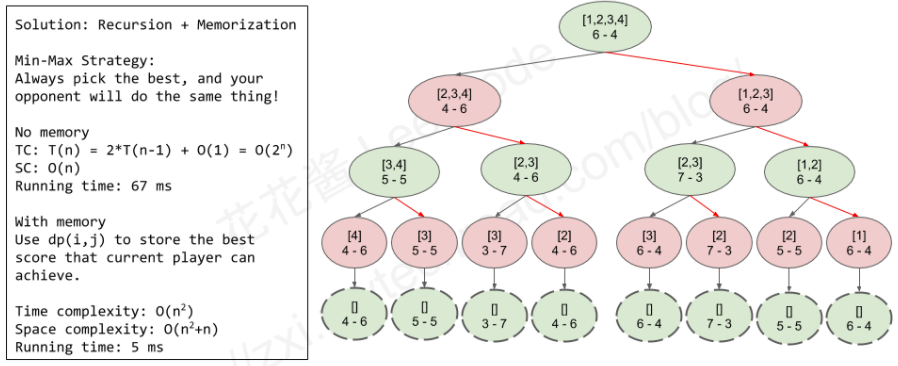
\includegraphics[width=.9\linewidth]{./pic/predictWinner.png}

\begin{minted}[fontsize=\scriptsize,linenos=false]{csharp}
private int helper( int [] arr, int i, int j) {
    if (i == j) return arr[i];
    else return Math.max(arr[i] - helper(arr, i+1, j), arr[j] - helper(arr, i, j-1));
}
public boolean PredictTheWinner(int[] nums) {
    int n = nums.length;
    if (n == 1) return true;
    return helper(nums, 0, n-1) >= 0;
}
\end{minted}

\subsection{1896. Minimum Cost to Change the Final Value of Expression - Hard}
\label{sec-1-4-43}
You are given a valid boolean expression as a string expression consisting of the characters '1','0','\&' (bitwise AND operator),'|' (bitwise OR operator),'(', and ')'.

For example, "()1|1" and "(1)\&()" are not valid while "1", "(((1))|(0))", and "1|(0\&(1))" are valid expressions.
Return the minimum cost to change the final value of the expression.

For example, if expression = "1|1|(0\&0)\&1", its value is 1|1|(0\&0)\&1 = 1|1|0\&1 = 1|0\&1 = 1\&1 = 1. We want to apply operations so that the new expression evaluates to 0.
The cost of changing the final value of an expression is the number of operations performed on the expression. The types of operations are described as follows:

Turn a '1' into a '0'.
Turn a '0' into a '1'.
Turn a '\&' into a '|'.
Turn a '|' into a '\&'.
Note: '\&' does not take precedence over '|' in the order of calculation. Evaluate parentheses first, then in left-to-right order.
\begin{minted}[fontsize=\scriptsize,linenos=false]{csharp}
private int [] getMinOperations(int va, int vb, int ca, int cb, char sign) {
    if (sign == '&') {
        if (va == 1 && vb == 1)      // 1&1, 将其中一个1反转为0
            return new int [] {1, Math.min(ca, cb)};
        else if (va == 0 && vb == 0) // 0&0, 将其中一个0反转为1,并将&反转为|
            return new int [] {0, Math.min(ca, cb) + 1};
        else return new int [] {0, 1}; // 1&0, 将&反转为|
    } else {
        if (va == 1 && vb == 1)        // 1|1,将其中一个1反转为0,并将|反转为&
            return new int [] {1, Math.min(ca, cb) + 1};
        else if (va == 0 && vb == 0)   // 0|0,将其中一个0反转为1
            return new int [] {0, Math.min(ca, cb)};
        else return new int [] {1, 1}; // 1|0,将|反转为&
    }
}
public int minOperationsToFlip(String expression) {
    Stack<Integer> res = new Stack<>();
    Stack<Character> sgn = new Stack<>();
    Stack<Integer> cnt = new Stack<>();
    for (char c : expression.toCharArray()) {
        if (c == '(' || c == '&' || c == '|') {
            sgn.push(c);
            continue;
        } else if (c == ')') sgn.pop();
        else {
            res.push((int)(c - '0'));
            cnt.push(1);
        }
        if (res.size() > 1 && sgn.peek() != '(') {
            int [] loc = getMinOperations(res.pop(), res.pop(), cnt.pop(), cnt.pop(), sgn.pop());
            res.push(loc[0]); // expr results
            cnt.push(loc[1]); // min operations
        }
    }
    return cnt.peek();
}
\end{minted}

\subsection{823. Binary Trees With Factors}
\label{sec-1-4-44}
Given an array of unique integers, arr, where each integer arr[i] is strictly greater than 1.
We make a binary tree using these integers, and each number may be used for any number of times. Each non-leaf node's value should be equal to the product of the values of its children.
Return the number of binary trees we can make. The answer may be too large so return the answer modulo 109 + 7.
\begin{minted}[fontsize=\scriptsize,linenos=false]{csharp}
public int numFactoredBinaryTrees(int[] arr) {
    int n = arr.length;
    Arrays.sort(arr);
    Map<Integer, Long> dp = new HashMap<>();
    int mod = 1_000_000_007;
    long res = 0;
    long max = 0;
    for (int i = 0; i < n; i++) {
        dp.put(arr[i], 1l);
        for (int j = 0; j < i; j++) {
            if (arr[i] % arr[j] == 0 && dp.containsKey(arr[i]/arr[j])) {
                max = dp.get(arr[i]) + dp.get(arr[j]) * dp.get(arr[i]/arr[j]);
                dp.put(arr[i], max % mod);
            }
        }
        res += dp.get(arr[i]);
        res %= mod;
    }
    return (int)(res % mod);
}
\end{minted}

\subsection{907. Sum of Subarray Minimums}
\label{sec-1-4-45}
Given an array of integers arr, find the sum of min(b), where b ranges over every (contiguous) subarray of arr. Since the answer may be large, return the answer modulo 109 + 7.
\begin{minted}[fontsize=\scriptsize,linenos=false]{csharp}
public int sumSubarrayMins(int[] arr) {
    int n = arr.length;
    // for each A[i], find k <= i <= j, so that A[i] is the min from [k,j]
    // sum += A[i] * (i-k+1) * (j-i+1)
    // so we need to find the next min to the right and to the left
    //这个过程可以简化为使用一个栈。对于被某个数从栈中弹出的数而言,它右侧第一个比它小的数就是这个数。所以我们可以对所有被弹出的数得到左侧的区间范围和右侧的区间范围。我觉得这是一种非常聪明的做法。 这个栈我看得稀里糊涂,再想一下
public int sumSubarrayMins(int[] a) { // 以每一个数为最小值找出左右边界。累加和
    int mod = (int)1e9 + 7;
    int n = a.length;
    int [] l = new int [n]; // 以每个当前数为最小值的左右最长边界
    int [] r = new int [n];
    ArrayDeque<Integer> s = new ArrayDeque<>();
    for (int i = 0; i < n; i++) {
        while (!s.isEmpty() && a[i] <= a[s.peek()]) // bug: a[i] < a[s.peek()]
            r[s.pop()] = i-1;
        s.push(i);
    }
    while (!s.isEmpty()) r[s.pop()] = n-1;
    for (int i = n-1; i >= 0; i--) {
        while (!s.isEmpty() && a[i] < a[s.peek()])
            l[s.pop()] = i+1;
        s.push(i);
    }
    while (!s.isEmpty()) 
        l[s.pop()] = 0;
    long sum = 0;
    long lcnt = 0, rcnt = 0;
    for (int i = 0; i < n; i++) {
        lcnt = i - l[i] + 1;
        rcnt = r[i] - i + 1;
        sum += a[i] * lcnt * rcnt;
        sum %= mod;
    }
    return (int)sum;
}
\end{minted}
\begin{enumerate}
\item 解题思路与分析
\label{sec-1-4-45-1}

思路是单调栈。开一个单调递增栈,里面存A AA中的数的下标,并且要保持下标对应的A AA的值单调递增。

遍历A AA,当遍历到A [ i ] A[i]A[i]的时候,如果栈不空并且栈顶t tt对应的值A [ t ] > A [ i ],那么我们就知道了A [ t ]作为最小值的最长的那个区间的左右端点,

先pop掉A [ t ] ,如果栈空了,说明左端点可以取到0 ,否则取栈顶加1(因为栈顶是A [ t ]左边第一个小于等于它的数的下标),而A [ i ] 是A [ t ]右边第一个小于它的数,所以右端点可以取到i − 1。

设左端点取l右端点取r,则以A [ t ]为最小值的区间的数量就是( t − l + 1 ) ( r − t + 1 ) 这么多,所以答案只需要累加一下A [ t ] × ( t − l + 1 ) ( r − t + 1 )即可。

\begin{minted}[fontsize=\scriptsize,linenos=false]{csharp}
public int sumSubarrayMins(int[] a) { // 将上面的三次遍历three passes变为一次遍历求结果
    int mod = (int)1e9 + 7;
    Deque<Integer> s = new ArrayDeque<>();
    long res = 0;
    for (int i = 0; i < a.length; i++) {
        while (!s.isEmpty() && a[i] < a[s.peek()]) { // 对于pop()出来的每一个数,计算出以它为最小值的左右边界,并累加和
            int pos = s.pop();                       // l和r是a[pos]左右数的选择数
            long l = pos - (s.isEmpty() ? -1 : s.peek()), r = i - pos;
            res += (l * r % mod) * a[pos] % mod;
            res %= mod;
        }
        s.push(i);
    }
    while (!s.isEmpty()) {
        int pos = s.pop();
        long l = pos - (s.isEmpty() ? -1 : s.peek()), r = a.length - pos;
        res += (l * r % mod) * a[pos] % mod;
        res %= mod;
    }
    return (int) res;
}
\end{minted}
\begin{itemize}
\item 上面的写法是包装出来的方法,用原始函数来写,效率狠好
\end{itemize}
\begin{minted}[fontsize=\scriptsize,linenos=false]{csharp}
private int MOD = (int)(1e9 + 7);
public int sumSubarrayMins(int[] arr) {
    int n = arr.length;
    Deque<Integer> dk = new LinkedList<>(); // 单调递增栈, 效率狠好!
    long res = 0;
    for (int i = 0; i < n; i++) {
        while (!dk.isEmpty() && arr[dk.peekLast()] > arr[i]) {
            int pkIdx = dk.pollLast();
            int stIdx;
            if (dk.isEmpty()) stIdx = -1;
            else stIdx = dk.peekLast();
            res += (long)arr[pkIdx] * (long)(i - pkIdx) * (long)(pkIdx - stIdx);
        }
        dk.offerLast(i);
    }
    while (!dk.isEmpty()) {
        int pkIdx = dk.pollLast();
        int stIdx;
        if (dk.isEmpty()) stIdx = -1;
        else stIdx = dk.peekLast();
        res += (long)arr[pkIdx] * (long)(n - pkIdx) * (long)(pkIdx - stIdx);
    }
    return (int)(res % MOD);
}
\end{minted}
\begin{itemize}
\item 找到的效率最高的写法
\end{itemize}
\begin{minted}[fontsize=\scriptsize,linenos=false]{csharp}
public int sumSubarrayMins(int[] arr) {
    int sum = 0;
    int mod = (int) 1e9 + 7;
    int curStVal = 0;
    Deque<int[]> s = new ArrayDeque<>(); // int [] {value, count}
    for (int i = 0; i < arr.length; i++) {
        int curCnt = 1;
        int curVal = arr[i];
        while (!s.isEmpty() && s.peek()[0] >= curVal) {
            int[] popped = s.pop();
            curStVal -= popped[1] * popped[0];
            curCnt += popped[1]; // assign all previous count to current
        }
        s.push(new int[]{curVal, curCnt});
        curStVal += curVal * curCnt;
        sum = (sum + curStVal) % mod;
    }
    return sum;
}
\end{minted}
\item 解题思路与分析: 另一种解法吧
\label{sec-1-4-45-2}
\begin{minted}[fontsize=\scriptsize,linenos=false]{csharp}
int mod = 1_000_000_007;
public int sumSubarrayMins(int[] arr) {
    int n = arr.length;
    long [] left = new long[n];
    long [] right = new long[n];
    long sum = 0;
    long cnt = 0;
    int j = 0;
    for (int i = 0; i < n; i++) { // 计算左边比自身大的数的个数
        cnt = 1;
        j = i-1;
        while (j >= 0 && arr[j] >= arr[i]) {
            cnt += left[j];
            j -= left[j];
        }
        left[i] = cnt;
    }
    // 就是因为计算了两个方向,所以对于数组里面有相同元素的情况下,需要特别考虑一下。
    //     不能重复计算, 也不能漏掉,
    //     具体就是一个方向的时候用<=, 另外一个方向的时候用<。 这个在做的时候也bug了。
    for (int i = n-1; i >= 0; i--) { // 计算右边比自身大的数的个数
        cnt = 1;
        j = i+1;
        while (j < n && arr[j] > arr[i]) {
            cnt += right[j];
            j += right[j];
        }
        right [i] = cnt;
    }
    for (int i = 0; i < n; i++) 
        sum += arr[i] * left[i] * right[i];
    return (int) (sum % mod);
}
\end{minted}
\end{enumerate}

\subsection{689. Maximum Sum of 3 Non-Overlapping Subarrays}
\label{sec-1-4-46}
Given an integer array nums and an integer k, find three non-overlapping subarrays of length k with maximum sum and return them.
Return the result as a list of indices representing the starting position of each interval (0-indexed). If there are multiple answers, return the lexicographically smallest one.
\begin{minted}[fontsize=\scriptsize,linenos=false]{csharp}
public int[] maxSumOfThreeSubarrays(int[] nums, int k) {
    int n = nums.length;
    int [] pre = new int [n+1];
    for (int i = 1; i <= n; i++) 
        pre[i] = pre[i-1] + nums[i-1];
    // left[i]表示在区间[0, i]范围内长度为k且和最大的子数组的起始位置
    // right[i]表示在区间[i, n - 1]范围内长度为k且和最大的子数组的起始位置
    int [] left = new int [n];
    int [] right = new int [n];
    int [] res = new int [3];
    Arrays.fill(right, n-k);
    for (int i = k, total = pre[k]-pre[0]; i < n; i++) {
        if (pre[i+1] - pre[i+1-k] > total) {
            left[i]= i+1-k;
            total = pre[i+1] - pre[i+1-k];
        } else left[i] = left[i-1];
    }
    for (int i = n-1-k, total = pre[n]-pre[n-k]; i >= 0; i--) {
        if (pre[i+k] - pre[i] >= total) {
            right[i] = i;
            total = pre[i+k] - pre[i];
        } else right[i] = right[i+1];
    }
    int max = Integer.MIN_VALUE;
    for (int i = k; i <= n-2*k; i++) {
        int l = left[i-1];
        int r = right[i+k];
        int total = (pre[i+k]-pre[i]) + (pre[k+l]-pre[l]) + (pre[r+k] - pre[r]);
        if (max < total) {
            max = total;
            res = new int [] {l, i, r};
        }
    }
    return res;
}
\end{minted}

\subsection{363. Max Sum of Rectangle No Larger Than K}
\label{sec-1-4-47}
Given an m x n matrix matrix and an integer k, return the max sum of a rectangle in the matrix such that its sum is no larger than k.
It is guaranteed that there will be a rectangle with a sum no larger than k.
\begin{enumerate}
\item 解题思路与分析: prefix sum在二维矩阵上的应用
\label{sec-1-4-47-1}

一维数组prefix sum在二维矩阵上的应用,考虑先降一下维度

\begin{minted}[fontsize=\scriptsize,linenos=false]{csharp}
// 把二维数组按行或列拆成多个一维数组,然后利用一维数组的累加和来找符合要求的数字,
// 这里用了 lower _ bound 来加快的搜索速度,也可以使用二分搜索法来替代。
public int maxSumSubmatrix(int[][] mat, int target) {
    int x = mat.length, y = mat[0].length, ans = Integer.MIN_VALUE;
    boolean flag = x <= y;
    int m = Math.min(x, y), n = Math.max(x, y);
    int [] sum = new int [n]; // 定义一维大的数组
    TreeSet<Integer> ts = new TreeSet<>();
    for (int i = 0; i < m; i++) { // 找从第 i 行开始一直到第 0 行这 i+1 行的可能组成的矩形长度
        Arrays.fill(sum, 0);
        for (int j = i; j >= 0; j--) { // 遍历行: 行的和的累加是通过每列列的和的累加sum数组的值来实现的
            ts.clear();
            ts.add(0);
            int cur = 0;
// 因为要满足 ( sum-set 中的元素) <=target,
// 而且 sum-set 中的元素的值要尽可能的大,sum - target <= setElement(要set中的元素,尽可能地小)
// 所以也就是在求大于等于 sum-target 中满足条件的元素的最小的一个
// 正好 TreeSet 中提供了这个方法 ceil() ,可以很方便的找出这个元素: 返回大于或等于e的最小元素;如果没有这样的元素,则返回null
            for (int k = 0; k < n; k++) { // 遍历列: 原始矩阵的行的和,或者是列的和,比较长的大的那一维的和
                if (flag) sum[k] += mat[j][k];
                else sum[k] += mat[k][j];
                cur += sum[k];
                Integer tmp = ts.ceiling(cur - target);
                if (tmp != null) ans = Math.max(ans, cur - tmp);
                ts.add(cur);
            }
        }
    }
    return ans;
}
+END_SRC
- 再稍微简洁一点儿的代码
#+BEGIN_SRC csharp
public int maxSumSubmatrix(int[][] mat, int target) { // 这么再看一下,就清清楚楚地啦
    int m = mat.length, n = mat[0].length, ans = Integer.MIN_VALUE;
    int M = Math.min(m, n), N = Math.max(m, n);
    for (int i = 0; i < M; i++) {
        int [] sum = new int [N];
        for (int j = i; j < M; j++) {
            TreeSet<Integer> ts = new TreeSet<>();
            int cur = 0;
            for (int k = 0; k < N; k++) {
                sum[k] += m > n ? mat[k][j] : mat[j][k];
                cur += sum[k];
                if (cur <= target) ans = Math.max(ans, cur);
                Integer tmp = ts.ceiling(cur - target);
                if (tmp != null) ans = Math.max(ans, cur - tmp);
                ts.add(cur);
            }
        }
    }
    return ans;
}
\end{minted}
\item 解题思路与分析: 暴力+优化
\label{sec-1-4-47-2}

这道题给了我们一个二维数组,让求和不超过的K的最大子矩形,那么首先可以考虑使用 brute force 来解,就是遍历所有的子矩形,然后计算其和跟K比较,找出不超过K的最大值即可。就算是暴力搜索,也可以使用优化的算法,比如建立累加和,参见之前那道题 Range Sum Query 2D - Immutable,可以快速求出任何一个区间和,下面的方法就是这样的,当遍历到 (i, j) 时,计算 sum(i, j),表示矩形 (0, 0) 到 (i, j) 的和,然后遍历这个矩形中所有的子矩形,计算其和跟K相比,这样既可遍历到原矩形的所有子矩形,参见代码如下:

\begin{minted}[fontsize=\scriptsize,linenos=false]{csharp}
public int maxSumSubmatrix(int[][] mat, int k) {
    int m = mat.length;
    int n = mat[0].length;
    if (m == 1 && n == 1) return mat[0][0];
    int [][] pre = new int [m][n];
    int res = Integer.MIN_VALUE;
    for (int i = 0; i < m; i++) {
        for (int j = 0; j < n; j++) {
            int t = mat[i][j];
            if (i > 0) t += pre[i-1][j];
            if (j > 0) t += pre[i][j-1];
            if (i > 0 && j > 0) t -= pre[i-1][j-1];
            pre[i][j] = t;
            for (int r = 0; r <= i; r++) {
                for (int c = 0; c <= j; c++) {
                    int d = pre[i][j];
                    if (r > 0) d -= pre[r-1][j];
                    if (c > 0) d -= pre[i][c-1];
                    if (r > 0 && c > 0) d += pre[r-1][c-1];
                    if (d <= k) res = Math.max(res, d);
                }
            }
        }
    }
    return res;
}
\end{minted}
\end{enumerate}

\subsection{1884. Egg Drop With 2 Eggs and N Floors - Medium}
\label{sec-1-4-48}
You are given two identical eggs and you have access to a building with n floors labeled from 1 to n.

You know that there exists a floor f where 0 <= f <= n such that any egg dropped at a floor higher than f will break, and any egg dropped at or below floor f will not break.

In each move, you may take an unbroken egg and drop it from any floor x (where 1 <= x <= n). If the egg breaks, you can no longer use it. However, if the egg does not break, you may reuse it in future moves.

Return the minimum number of moves that you need to determine with certainty what the value of f is.
\begin{minted}[fontsize=\scriptsize,linenos=false]{csharp}
    // 思路: https://zhuanlan.zhihu.com/p/41257286 可以借这个思路理解一下
    // DP[i][j]表示用i个鸡蛋,j层楼的情况下最坏情况下所需扔鸡蛋的最少数目。
    // 可知初始条件为:
    // DP[1][0] = 0; DP[2][0] = 0;
    // DP[1][1] = 1; DP[2][1] = 1;
    // DP[1][i] = i; //i = 1 … n
    // 对于DP[2][i], i = 2 … n的情况,我们可以这样考虑:
    //     遍历j=2…i,求DP[2][j],分两种情况:
    //     如果第1个鸡蛋在第j-1层摔破了,则我们在第j层只需摔第2个鸡蛋一次即可,此时总摔鸡蛋数为DP[1][j-1]+1。
    //     注意上面的1是因为第j层需要摔第2个鸡蛋1次。为什么DP[1][j-1]不能写成1呢?因为第1个鸡蛋在第j-1层摔破了,我们不能肯定在第1,2,…,j-2层不会破,所以要用DP[1][j-1]。
    //     如果第1个鸡蛋在第j-1层没有摔破,则我们在第j到i层有2个鸡蛋可以摔,此时退化到DP[2][i-j]的情况。该种情形下总共扔1+DP[2][i-j]。那个1就是表示第1个鸡蛋在第j-1层扔了1次。这里我们为什么只考虑用1,而不用考虑DP[1][j-1]呢?因为如果第j-1层没有摔破,第1,2,…,j-2层也就不用考虑了。
    //     因为是求最坏情况下的数目,所以DP[2][j]=1 + max(DP[1][j-1]+1, DP[2][i-j])。
    //     而我们是要求所有最坏情况下的最少数目,所以DP[2][j]=min(1 + max(DP[1][j-1]+1, DP[2][i-j]))。i = 2…n, j = 2…i。
public int twoEggDrop(int n) { // 1 + 2 + 3 + ... + x >= n ==> get x
    if (n <= 1) return n;
    int [][] dp = new int [3][n+1]; // DP[i][j]表示用i个鸡蛋,j层楼的情况下最坏情况下所需扔鸡蛋的最少数目。
    for (int i = 0; i < 3; i++) 
        Arrays.fill(dp[i], Integer.MAX_VALUE);
    dp[1][0] = 0;
    dp[1][1] = 1;
    dp[2][0] = 0;
    dp[2][1] = 1;
    for (int i = 1; i <= n; i++) dp[1][i] = i;
    for (int i = 2; i <= n; i++) 
        for (int j = 2; j <= i; j++) 
            dp[2][i] = Math.min(dp[2][i], 1 + Math.max(dp[1][j-1], dp[2][i-j])); // 1: 这个鸡蛋在j-i层扔了一次,要统计入结果
    return dp[2][n];
}
public int twoEggDrop(int n) { // 1 + 2 + 3 + ... + x >= n ==> get x
    if (n <= 2) return n;
    return (int)(Math.ceil((-1 + Math.sqrt((long)n * 8 + 1)) / 2.0));
}
\end{minted}
\subsection{887. Super Egg Drop - Hard}
\label{sec-1-4-49}
You are given k identical eggs and you have access to a building with n floors labeled from 1 to n.

You know that there exists a floor f where 0 <= f <= n such that any egg dropped at a floor higher than f will break, and any egg dropped at or below floor f will not break.

Each move, you may take an unbroken egg and drop it from any floor x (where 1 <= x <= n). If the egg breaks, you can no longer use it. However, if the egg does not break, you may reuse it in future moves.

Return the minimum number of moves that you need to determine with certainty what the value of f is.
\begin{enumerate}
\item 解题思路与分析
\label{sec-1-4-49-1}
\begin{itemize}
\item \url{https://charlesliuyx.github.io/2018/10/11/\%E3\%80\%90\%E7\%9B\%B4\%E8\%A7\%82\%E7\%AE\%97\%E6\%B3\%95\%E3\%80\%91Egg\%20Puzzle\%20\%E9\%B8\%A1\%E8\%9B\%8B\%E9\%9A\%BE\%E9\%A2\%98/}
\item \url{https://www.shuzhiduo.com/A/D8548M4Q5E/}
\end{itemize}
\item 解题思路与分析
\label{sec-1-4-49-2}
1 <= K <= 100, 
1 <= N <= 10000

这道题说给了我们K个鸡蛋,还有一栋共N层的大楼,说是鸡蛋有个临界点的层数F,高于这个层数扔鸡蛋就会碎,否则就不会,问我们找到这个临界点最小需要多少操作,注意这里的操作只有当前还有没碎的鸡蛋才能进行。这道题是基于经典的扔鸡蛋的问题改编的,原题是有 100 层楼,为了测鸡蛋会碎的临街点,最少可以扔几次?答案是只用扔 14 次就可以测出来了,讲解可以参见[油管上的这个视频](\url{https://www.youtube.com/watch?v=NGtt7GJ1uiM}),这两道题看着很相似,其实是有不同的。这道题限制了鸡蛋的个数K,假设我们只有1个鸡蛋,碎了就不能再用了,这时我们要测 100 楼的临界点的时候,只能一层一层去测,当某层鸡蛋碎了之后,就知道临界点了,所以最坏情况要测 100 次,注意要跟经典题目中扔 14 次要区分出来。那么假如有两个鸡蛋呢,其实需要的次数跟经典题目中的一样,都是 14 次,这是为啥呢?因为在经典题目中,我们是分别间隔 14,13,12,\ldots{},2,1,来扔鸡蛋的,当我们有两个鸡蛋的时候,我们也可以这么扔,第一个鸡蛋仍在 14 楼,若碎了,说明临界点一定在 14 楼以内,可以用第二个鸡蛋去一层一层的测试,所以最多操作 14 次。若第一个鸡蛋没碎,则下一次扔在第 27 楼,假如碎了,说明临界点在 (14,27] 范围内,用第二个鸡蛋去一层一层测,总次数最多 13 次。若第一个鸡蛋还没碎,则继续按照 39, 50, \ldots{}, 95, 99,等层数去测,总次数也只可能越来越少,不会超过 14 次的。但是照这种思路分析的话,博主就不太清楚有3个鸡蛋,在 100 楼测,最少的步骤数,答案是9次,博主不太会分析怎么测的,各位看官大神知道的话一定要告诉博主啊。

其实这道题比较好的解法是用动态规划 Dynamic Programming,因为这里有两个变量,鸡蛋数K和楼层数N,所以就要使用一个二维数组 DP,其中 dp[i][j] 表示有i个鸡蛋,j层楼要测需要的最小操作数。那么我们在任意k层扔鸡蛋的时候就有两种情况(注意这里的k跟鸡蛋总数K没有任何关系,k的范围是 [1, j]):
\begin{minted}[fontsize=\scriptsize,linenos=false]{csharp}
鸡蛋碎掉:接下来就要用 i-1 个鸡蛋来测 k-1 层,所以需要 dp[i-1][k-1] 次操作。
鸡蛋没碎:接下来还可以用i个鸡蛋来测 j-k 层,所以需要 dp[i][j-k] 次操作。
\end{minted}

因为我们每次都要面对最坏的情况,所以在第j层扔,需要 max(dp[i-1][k-1], dp[i][j-k])+1 步,状态转移方程为:

dp[i][j] = min(dp[i][j], max(dp[i - 1][k - 1], dp[i][j - k]) + 1) ( 1 <= k <= j )

\begin{minted}[fontsize=\scriptsize,linenos=false]{csharp}
public int superEggDrop(int k, int n) { // tle:  O(KN^2) 还需要优化一下
    if (k < 1 || n < 1) return 0;
    int [] pre = new int [n+1]; //上一层备忘录,存储鸡蛋数量-1的n层楼条件下的最优化尝试次数
    int [] cur = new int [n+1]; // 当前备忘录,存储当前鸡蛋数量的n层楼条件下的最优化尝试次数
    for (int i = 1; i <= n; i++) // 把备忘录每个元素初始化成最大的尝试次数
        cur[i] = i;
    for (int i = 2; i <= k; i++) {
        pre = cur.clone(); // 当前备忘录拷贝给上一次备忘录,并重新初始化当前备忘录
        for (int j = 1; j <= n; j++) cur[j] = j;
        for (int j = 1; j <= n; j++) // 需要想办法去优化时间复杂度。这种写法里面我们枚举了 [1, j] 范围所有的k值,总时间复杂度为 O(KN^2),
            for (int x = 1; x < j; x++) 
// 扔鸡蛋的楼层从1到m枚举一遍,如果当前算出的尝试次数小于上一次算出的尝试次数,则取代上一次的尝试次数。
// 这里可以打印k的值,从而知道第一个鸡蛋是从第几次扔的。
                cur[j] = Math.min(cur[j], 1 + Math.max(pre[x-1], cur[j-x]));
    }
    return cur[n];
}
\end{minted}

这种写法会超时 Time Limit Exceeded,代码请参见评论区1楼,OJ 对时间卡的还是蛮严格的,所以我们就需要想办法去优化时间复杂度。这种写法里面我们枚举了 [1, j] 范围所有的k值,总时间复杂度为 O(KN\^{}2),若我们仔细观察 dp[i - 1][k - 1] 和 dp[i][j - k],可以发现前者是随着k递增,后者是随着k递减,且每次变化的值最多为1,所以只要存在某个k值使得二者相等,那么就能得到最优解,否则取最相近的两个k值做比较,由于这种单调性,我们可以在 [1, j] 范围内对k进行二分查找,找到第一个使得 dp[i - 1][k - 1] 不小于 dp[i][j - k] 的k值,然后用这个k值去更新 dp[i][j] 即可,这样时间复杂度就减少到了 O(KNlgN),其实也是险过,参见代码如下:

\begin{minted}[fontsize=\scriptsize,linenos=false]{csharp}
// 若我们仔细观察 dp[i - 1][k - 1] 和 dp[i][j - k],可以发现前者是随着k递增,后者是随着k递减,且每次变化的值最多为1,
// 所以只要存在某个k值使得二者相等,那么就能得到最优解,否则取最相近的两个k值做比较,
// 由于这种单调性,我们可以在 [1, j] 范围内对k进行二分查找,找到第一个使得 dp[i - 1][k - 1] 不小于 dp[i][j - k] 的k值,然后用这个k值去更新 dp[i][j] 即可,
// 这样时间复杂度就减少到了 O(KNlgN)
public int superEggDrop(int k, int n) { // O(KNlgN)
    int [][] dp = new int [k+1][n+1];
    for (int i = 1; i <= n; i++) dp[1][i] = i; // 把只有一个鸡蛋的情况初始化为最大值
    for (int i = 2; i <= k; i++) {
        for (int j = 1; j <= n; j++) {
            dp[i][j] = j;
            int l = 1, r = j, m = 0;
            while (l < r) {
                m = (l + r) / 2;
                if (dp[i-1][m-1] < dp[i][j-m]) l = m + 1; // < 左边随m递增,< 右边随m递减,这个性质在这里很重要,所以可以二分查找
                else r = m;
            } // 这里查找的右边界也注意一下
            dp[i][j] = Math.min(dp[i][j], Math.max(dp[i-1][r-1], dp[i][j-r]) + 1); // 用这个鸡蛋测试了一次了
        }
    }
    return dp[k][n];
}
\end{minted}

进一步来想,对于固定的k,dp[i][j-k] 会随着j的增加而增加,最优决策点也会随着j单调递增,所以在每次移动j后,从上一次的最优决策点的位置来继续向后查找最优点即可,这样时间复杂度就优化到了 O(KN),我们使用一个变量s表示当前的j值下的的最优决策点,然后当j值改变了,我们用一个 while 循环,来找到第下一个最优决策点s,使得 dp[i - 1][s - 1] 不小于 dp[i][j - s],参见代码如下:

\begin{minted}[fontsize=\scriptsize,linenos=false]{csharp}
public int superEggDrop(int k, int n) { // O(KN)
    int [][] dp = new int [k+1][n+1];
    for (int i = 1; i <= n; i++) dp[1][i] = i; // 把只有一个鸡蛋的情况初始化为最大值
    for (int i = 2; i <= k; i++) {
        int s = 1; // k
        for (int j = 1; j <= n; j++) { // n
            dp[i][j] = j;
            while (s < j && dp[i-1][s-1] < dp[i][j-s]) s++; // 因为单调性,s一直向右滑动,总共执行n次
            dp[i][j] = Math.min(dp[i][j], Math.max(dp[i-1][s-1], dp[i][j-s]) + 1);
        }
    }
    return dp[k][n];
}
\end{minted}

其实我们还可以进一步优化时间复杂度到 O(KlgN),不过就比较难想到了,需要将问题转化一下,变成已知鸡蛋个数,和操作次数,求最多能测多少层楼的临界点。还是使用动态规划 Dynamic Programming 来做,用一个二维 DP 数组,其中 dp[i][j] 表示当有i次操作,且有j个鸡蛋时能测出的最高的楼层数。再来考虑状态转移方程如何写,由于 dp[i][j] 表示的是在第i次移动且使用第j个鸡蛋测试第 dp[i-1][j-1]+1 层,因为上一个状态是第i-1次移动,且用第j-1个鸡蛋。此时还是有两种情况:

鸡蛋碎掉:说明至少可以测到的不会碎的层数就是 dp[i-1][j-1]。

鸡蛋没碎:那这个鸡蛋可以继续利用,此时我们还可以再向上查找 dp[i-1][j] 层。

那么加上当前层,总共可以通过i次操作和j个鸡蛋查找的层数范围是 [0, dp[i-1][j-1] + dp[i-1][j] + 1],这样就可以得到状态转移方程如下:

dp[i][j] = dp[i - 1][j - 1] + dp[i - 1][j] + 1

当 dp[i][K] 正好小于N的时候,i就是我们要求的最小次数了,参见代码如下:

\begin{minted}[fontsize=\scriptsize,linenos=false]{csharp}
public int superEggDrop(int k, int n) { // O(KlgN): 为什么说这里就是 O(klgN)呢?因为dp[m][k]的增长呈指数级的?
    int [][] dp = new int [n+1][k+1]; // 在第 i 次移动且使用第 j 个鸡蛋测试第 dp[i-1][j-1]+1 层
    int m = 0; // 最小测试次数
    while (dp[m][k] < n) { // 当dp[m][k] == n,退出循环的时候,m就是要求的最小操作次数了
        ++m;
        for (int j = 1; j <= k; j++) 
            dp[m][j] = dp[m-1][j-1] + dp[m-1][j] + 1; // 分上一次测的 第j-1个鸡蛋 碎了 和 没有碎 两种情况来更新当前值
    }
    return m;
}
\end{minted}

我们可以进一步的优化空间,因为当前的操作次数值的更新只跟上一次操作次数有关,所以我们并不需要保存所有的次数,可以使用一个一维数组,其中 dp[i] 表示当前次数下使用i个鸡蛋可以测出的最高楼层。状态转移方程的推导思路还是跟上面一样,参见代码如下:
\begin{minted}[fontsize=\scriptsize,linenos=false]{csharp}
public int superEggDrop(int k, int n) { // O(KlgN): 空间压缩
    int [] dp = new int [k+1]; // dp[i] 表示当前次数下使用 i 个鸡蛋可以测出的最高楼层
    int ans = 0;
    for (; dp[k] < n; ans++) // 压缩代码到一行
        for (int i = k; i >= 1; i--) // 压缩空间后,因为是想要根据上一行[ans-1]时的i-1/i来更新当前结果,需要倒序遍历以免产生脏数据
            dp[i] = dp[i] + dp[i-1] + 1;
    return ans;
}
\end{minted}

下面这种方法就非常的 tricky 了,居然推导出了使用k个鸡蛋,移动x次所能测的最大楼层数的通项公式,推导过程可以参见[这个帖子](\url{https://leetcode.com/problems/super-egg-drop/discuss/181702/Clear-C\%2B\%2B-codeRuntime-0-msO(1)}-spacewith-explation.No-DPWhat-we-need-is-mathematical-thought!),通项公式如下:

f(k,x) = x(x-1)..(x-k)/k! + \ldots{} + x(x-1)(x-2)/3! + x(x-1)/2! + x

这数学功底也太好了吧,有了通向公式后,我们就可以通过二分搜索法 Binary Search 来快速查找满足题目的x。这里其实是博主之前总结贴 [LeetCode Binary Search Summary 二分搜索法小结](\url{http://www.cnblogs.com/grandyang/p/6854825.html}) 中的第四类,用子函数当作判断关系,这里子函数就是用来实现上面的通向公式的,不过要判断,当累加和大于等于N的时候,就要把当的累加和返回,这样相当于进行了剪枝,因为在二分法中只需要知道其跟N的大小关系,并不 care 到底大了多少,这样快速定位x的方法运行速度貌似比上面的 DP 解法要快不少,但是这通项公式尼玛谁能容易的推导出来,只能膜拜叹服了,参见代码如下:

\begin{minted}[fontsize=\scriptsize,linenos=false]{csharp}
public int superEggDrop(int k, int n) { // O(KlgN):数学推导找出了推理公式,速度最快
    int l = 1, r = n;
    while (l < r) { // 寻找右边界
        int m = l + (r - l) / 2;
        if (helper(m, k, n) < n) l = m + 1;
        else r = m;
    }
    return r;
}
int helper(int m, int k, int n) { // 能查找到的最大楼层数
    int ans = 0, r = 1;
    for (int i = 1; i <= k; i++) {
        r *= m - i + 1;
        r /= i;
        ans += r;
        if (ans >= n) break;
    }
    return ans;
}
\end{minted}
\end{enumerate}

\subsection{1981. Minimize the Difference Between Target and Chosen Elements}
\label{sec-1-4-50}
You are given an m x n integer matrix mat and an integer target.
Choose one integer from each row in the matrix such that the absolute difference between target and the sum of the chosen elements is minimized.
Return the minimum absolute difference.
The absolute difference between two numbers a and b is the absolute value of a - b.
\begin{minted}[fontsize=\scriptsize,linenos=false]{csharp}
// DP + BitSet : 这里面有个小问题需要挑出来
// 使用一个DP数组存下当前行和之前行每行选一个数可能构成的和,
// 在本题中,可以使用BitSet(简介)来存储之前行可以组成的和(由于所有数的最大值为70,而行数最大也为70,故BitSet最大的位数即为4900)。
// 对于当前行,遍历BitSet已经set过的位(即代表之前行可能组成的和),然后加上当前数,set新的和
// 最后遍历BitSet,求出当前位与target的最小值
public int minimizeTheDifference(int[][] mat, int target) {
    int m = mat.length;
    int n = mat[0].length;
    BitSet sum = new BitSet(); // 遍历每一行,存下当前行和之前行可能组成的和
    for (int i = 0; i < n; i++) // 初始时存下第一行
        sum.set(mat[0][i]);
    for (int i = 1; i < m; i++) {
        BitSet newSum = new BitSet(); // 用来存新的和
        for (int j = 0; j < n; j++) {
            // 注意:要遍历BitSet中的真实位,请使用以下循环:previousSetBit()方法 用于查找在指定的起始索引上或之前是否存在任何真位
            // for (int i = bs.length(); (i = bs.previousSetBit(i-1)) >= 0; ) {
            //     // operate on index i here
            // }
            for (int k = sum.length(); (k = sum.previousSetBit(k-1)) >= 0; ) {
                newSum.set(k+mat[i][j]);
            }
        }
        sum = newSum;
    }
    int ans = 4900;
    for (int k = sum.length(); (k = sum.previousSetBit(k-1)) >= 0;) {
        int diff = Math.abs(k - target);
        ans = Math.min(ans, diff);
    }
    return ans;
}
public int minimizeTheDifference(int[][] mat, int target) {
    int m = mat.length;
    int n = mat[0].length;
    int diff = Integer.MAX_VALUE, limit = 4900;
    int [] dp = new int[limit];
    for (int i = 0; i < n; i++) // 相当于是手工实现java BitSet
        dp[mat[0][i]] = 1;
    for (int i = 1; i < m; i++) {
        int [] tmp = new int [limit];
        for (int v = limit-1; v >= 0; v--) {
            if (dp[v] == 0) continue;
            for (int j = 0; j < n; j++) {
                if (v + mat[i][j] < limit)
                    tmp[v+mat[i][j]] = 1;
            }
        }
        System.arraycopy(tmp, 0, dp, 0, dp.length);
    }
    for (int i = 0; i < limit; i++) 
        if (dp[i] > 0) diff = Math.min(diff, Math.abs(i-target));
    return diff;  // min difference
}
\end{minted}

\subsection{801. Minimum Swaps To Make Sequences Increasing - Hard}
\label{sec-1-4-51}
You are given two integer arrays of the same length nums1 and nums2. In one operation, you are allowed to swap nums1[i] with nums2[i].

For example, if nums1 = [1,2,3,8], and nums2 = [5,6,7,4], you can swap the element at i = 3 to obtain nums1 = [1,2,3,4] and nums2 = [5,6,7,8].
Return the minimum number of needed operations to make nums1 and nums2 strictly increasing. The test cases are generated so that the given input always makes it possible.

An array arr is strictly increasing if and only if arr\footnotemark[1]{} < arr\footnotemark[2]{} < arr\footnotemark[3]{} < \ldots{} < arr[arr.length - 1].
\begin{minted}[fontsize=\scriptsize,linenos=false]{csharp}
// 设 dp[0][i] 表示不交换 A[i] 和 B[i] 在下标 i 的交换次数
// 设 dp[1][i] 表示交换 A[i] 和 B[i] 在下标 i 的交换次数
// 可以看到交换与否只取决与前一个状态, 可以将空间复杂度压缩到 O(1)
//     时间复杂度为 O(n), 空间复杂度为 O(1)
public int minSwap(int[] a, int[] b) {
    int n = a.length;
    int [][] dp = new int [2][n];
    for (int [] row : dp) 
        Arrays.fill(row, Integer.MAX_VALUE);
    dp[0][0] = 0;
    dp[1][0] = 1;
    for (int i = 1; i < n; i++) {
        if (a[i] > a[i-1] && b[i] > b[i-1]) {
            dp[0][i] = Math.min(dp[0][i], dp[0][i-1]);    // 不需要交换不用增加交换次数
            dp[1][i] = Math.min(dp[1][i], dp[1][i-1] + 1);// 如果要交换前一个也必须交换才能满足递增的条件
        }
        if (a[i] > b[i-1] && b[i] > a[i-1]) {
            dp[0][i] = Math.min(dp[0][i], dp[1][i-1]);    // 表示 i - 1 位置发生交换  
            dp[1][i] = Math.min(dp[1][i], dp[0][i-1] + 1);// 表示在 i - 1 不换的基础上, i 发生了交换 
        }
    }
    return Math.min(dp[0][n-1], dp[1][n-1]);
}
\end{minted}
\subsection{837. New 21 Game - Medium}
\label{sec-1-4-52}
Alice plays the following game, loosely based on the card game "21".

Alice starts with 0 points and draws numbers while she has less than k points. During each draw, she gains an integer number of points randomly from the range [1, maxPts], where maxPts is an integer. Each draw is independent and the outcomes have equal probabilities.

Alice stops drawing numbers when she gets k or more points.

Return the probability that Alice has n or fewer points.

Answers within 10-5 of the actual answer are considered accepted.
\begin{minted}[fontsize=\scriptsize,linenos=false]{csharp}
// When the draws sum up to K, it stops, calculate the possibility K<=sum<=N.
//     Think about one step earlier, sum = K-1, game is not ended and draw largest card W.
//     K-1+W is the maximum sum could get when game is ended. If it is <= N, then for sure the possiblity when games end ans sum <= N is 1.
//     Because the maximum is still <= 1.
//     Otherwise calculate the possibility sum between K and N.
//     Let dp[i] denotes the possibility of that when game ends sum up to i.
//     i is a number could be got equally from i - m and draws value m card.
//     Then dp[i] should be sum of dp[i-W] + dp[i-W+1] + ... + dp[i-1], devided by W.
//     We only need to care about previous W value sum, accumlate winSum, reduce the possibility out of range.
//     Time Complexity: O(N).
//     Space: O(N).
public double new21Game(int n, int k, int w) { // k : threshold
    if (k == 0 || n >= (k + w)) return 1.0;
    if (k > n) return 0;
    double [] dp = new double [n+1];
    dp[0] = 1.0;
    double winSum = 1;
    double res = 0;
    for (int i = 1; i <= n; i++) {
        dp[i] = winSum / w;
        if (i < k) winSum += dp[i];
        else res += dp[i];
        if (i >= w) winSum -= dp[i-w];
    }
    return res;
}
\end{minted}
\subsection{1105. Filling Bookcase Shelves - Medium}
\label{sec-1-4-53}
You are given an array books where books[i] = [thicknessi, heighti] indicates the thickness and height of the ith book. You are also given an integer shelfWidth.

We want to place these books in order onto bookcase shelves that have a total width shelfWidth.

We choose some of the books to place on this shelf such that the sum of their thickness is less than or equal to shelfWidth, then build another level of the shelf of the bookcase so that the total height of the bookcase has increased by the maximum height of the books we just put down. We repeat this process until there are no more books to place.

Note that at each step of the above process, the order of the books we place is the same order as the given sequence of books.

For example, if we have an ordered list of 5 books, we might place the first and second book onto the first shelf, the third book on the second shelf, and the fourth and fifth book on the last shelf.
Return the minimum possible height that the total bookshelf can be after placing shelves in this manner.
\begin{minted}[fontsize=\scriptsize,linenos=false]{csharp}
// 求摆放前i本书需要的最小高度,首先需要求摆放前i-1书需要的最小高度,以此类推,最初需要计算的是摆放第0本书需要的最小高度,也就是0。
// 根据前i-1本书求前i书需要的最小高度的思路是:
// 尝试①将第i本书放在前i-1本书的下面
// 以及②将前i-1本书的最后几本和第i本书放在同一层两种方案,看哪种方案高度更小就用哪种方案,依次求出摆放前1,…,n本书需要的最小高度。
public int minHeightShelves(int[][] books, int shelfWidth) {
    int [] dp = new int [books.length + 1];
    for (int i = 1; i < dp.length; i++) { // 依次求摆放前i本书的最小高度
        int width = books[i-1][0];
        int height = books[i-1][1];
        dp[i] = dp[i-1] + height;
        // 将前i - 1本书从第i - 1本开始放在与i同一层,直到这一层摆满或者所有的书都摆好
        for (int j = i-1; j > 0 && width + books[j-1][0] <= shelfWidth; j--) {
            height = Math.max(height, books[j-1][1]); // 每层的高度由最高的那本书决定
            width += books[j-1][0];
            dp[i] = Math.min(dp[i], dp[j-1] + height);// 选择高度最小的方法
        }
    }            
    return dp[books.length];
}
\end{minted}
\begin{itemize}
\item 后来又出的bug
\end{itemize}
\begin{minted}[fontsize=\scriptsize,linenos=false]{csharp}
public int minHeightShelves(int [][] b, int w) { 
    int n = b.length, curLayerWidth = 0, max = 0;
    int [] dp = new int [n+1];
    Arrays.fill(dp, n+1);
    dp[0] = 0;
    for (int i = 1; i <= n; i++) {   // 依次求摆放前i本书的最小高度
        dp[i] = dp[i-1] + b[i-1][1]; // 初始化为最大值:单列一行,再看之前的行有没有空隙可以放入之前的层?
        curLayerWidth = b[i-1][0];
         max = b[i-1][1];
        for (int j = i-1; j > 0 && curLayerWidth + b[j-1][0] <= w; j--) { // 将前i - 1本书从第i - 1本开始放在与i同一层,直到这一层摆满或者所有的书都摆好
            curLayerWidth += b[j-1][0];
            max = Math.max(max, b[j-1][1]);
            // dp[i] = Math.min(dp[i], dp[j] + max);  // bug: dp[j] + max 是从第j本开始,包括第j本,这与之后的书放到最后一层所能形成的最小高度
            dp[i] = Math.min(dp[i], dp[j - 1] + max); // 所以,是用j之前所开成的最小高度,dp[j-1]加上最后一层所能形成的最小高度
        }
    }
    return dp[n];
}
\end{minted}
\subsection{790. Domino and Tromino Tiling}
\label{sec-1-4-54}
You have two types of tiles: a 2 x 1 domino shape and a tromino shape. You may rotate these shapes.

Given an integer n, return the number of ways to tile an 2 x n board. Since the answer may be very large, return it modulo 109 + 7.

In a tiling, every square must be covered by a tile. Two tilings are different if and only if there are two 4-directionally adjacent cells on the board such that exactly one of the tilings has both squares occupied by a tile.
\begin{enumerate}
\item 解题思路与分析
\label{sec-1-4-54-1}

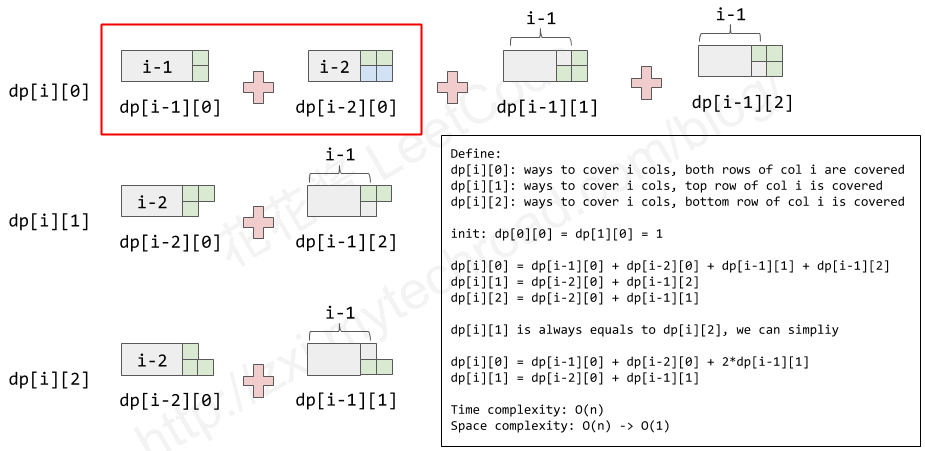
\includegraphics[width=.9\linewidth]{./pic/790.png}

\begin{minted}[fontsize=\scriptsize,linenos=false]{csharp}
public int numTilings(int n) {
    int mod = (int)1e9 + 7;
    int [][] dp = new int [n+1][2];
    dp[0][0] = 1;
    dp[1][0] = 1;
    for (int i = 2; i <= n; i++) {
        dp[i][0] = (int)((dp[i-1][0] + dp[i-2][0]) % mod + (2 * dp[i-1][1]) % mod) % mod;
        dp[i][1] = (int)(dp[i-2][0] + dp[i-1][1]) % mod;
    }
    return dp[n][0];
}
\end{minted}
\end{enumerate}
\subsection{1997. First Day Where You Have Been in All the Rooms - Medium}
\label{sec-1-4-55}
There are n rooms you need to visit, labeled from 0 to n - 1. Each day is labeled, starting from 0. You will go in and visit one room a day.

Initially on day 0, you visit room 0. The order you visit the rooms for the coming days is determined by the following rules and a given 0-indexed array nextVisit of length n:

Assuming that on a day, you visit room i,
if you have been in room i an odd number of times (including the current visit), on the next day you will visit a room with a lower or equal room number specified by nextVisit[i] where 0 <= nextVisit[i] <= i;
if you have been in room i an even number of times (including the current visit), on the next day you will visit room (i + 1) mod n.
Return the label of the first day where you have been in all the rooms. It can be shown that such a day exists. Since the answer may be very large, return it modulo 109 + 7.
\begin{minted}[fontsize=\scriptsize,linenos=false]{csharp}
public int firstDayBeenInAllRooms(int [] nextVisit) {
    int n = nextVisit.length, mod = (int)1e9 + 7;
    long [] dp = new long [n];
    dp[0] = 0;
    for (int i = 1; i < n; i++) 
        dp[i] = (2 * dp[i-1] % mod + mod - dp[nextVisit[i-1]] + 2) % mod;
    return (int)dp[n-1];
}
\end{minted}

\subsection{943. Find the Shortest Superstring - Hard}
\label{sec-1-4-56}
Given an array of strings words, return the smallest string that contains each string in words as a substring. If there are multiple valid strings of the smallest length, return any of them.

You may assume that no string in words is a substring of another string in words.
\begin{itemize}
\item 深搜 + 记忆数组 + 裁枝
\end{itemize}
\begin{minted}[fontsize=\scriptsize,linenos=false]{csharp}
public String shortestSuperstring(String [] sa) { // 回塑: 暴搜+剪枝,但回塑仍然是最慢的方法
    n = sa.length;
    max = new int [n][n];
    for (int i = 0; i < n; i++) 
        for (int j = 0; j < n; j++) {
            if (i == j) continue;
            for (int k = Math.min(sa[i].length(), sa[j].length()); k >= 1; k--) // 不想遍历所有,找到一个有效最优解,就剪枝中断
                if (sa[i].substring(sa[i].length()-k).equals(sa[j].substring(0, k))) {
                    max[i][j] = k; // sa[i] 的尾 与 sa[j]的头的 最长公共后前缀 长度
                    break;
                }
        }                
    dp = new int [1 << n][n];
    ans = new int [n]; // 最终答案: 最小长度的字符串下标位置
    vis = new boolean [n];
    dfs(new int [n], 0, 0, 0);
    String s = sa[ans[0]];
    for (int i = 1; i < n; i++) { // 当前字符串的前缀已经被上一个字符串的后缀cover了,所以只取后没被覆盖住的后半部分
        int cmnLen = max[ans[i-1]][ans[i]];
        s += sa[ans[i]].substring(cmnLen);
    }
    return s;
}
int [][] dp;
int [][] max; // max common length between two strings
boolean [] vis;
int n, maxLen = Integer.MIN_VALUE; // BUG: has to be initialized 
int [] ans;
private void dfs(int [] a, int idx, int sum, int state) {
    if (idx == n) {
        if (sum > maxLen) {
            maxLen = sum;
            // ans = Arrays.copyOf(a, n);
            ans = a.clone(); // 效果一样
        }
        return ;
    }
    for (int i = 0; i < n; i++) {
        if (vis[i]) continue;
        int mask = state | (1 << i);
        int curLen = sum + (idx == 0 ? 0 : max[a[idx-1]][i]);
        if (dp[mask][i] > 0 && dp[mask][i] >= curLen) continue; // == 的情况可以剪枝,因为dp[][]本来就是记忆着各路径状态下的全局最优解,不能更优就剪掉
        vis[i] = true;
        a[idx] = i;
        dp[mask][i] = curLen; // BUG: 需要这一行记忆化,加速搜索与剪枝,重中之重不可记忆, otherwise tle !!!
        dfs(a, idx+1, curLen, mask);
        vis[i] = false;
    }
}
\end{minted}
\begin{itemize}
\item 动态规划
\end{itemize}
\begin{minted}[fontsize=\scriptsize,linenos=false]{csharp}
public String shortestSuperstring(String[] s) {
    int n = s.length;
    String [][] dp = new String [1 << n][n]; // 这个dp的设计还比较新颖奇特:
    int [][] max = new int [n][n];
    for (int i = 0; i < n; i++) 
        for (int j = 0; j < n; j++) {
            if (i == j) continue;
            for (int k = Math.min(s[i].length(), s[j].length()); k >= 1; k--) 
                 if (s[i].substring(s[i].length()-k).equals(s[j].substring(0, k))) {
                    max[i][j] = k;
                    break;
                }
        }
    for (int i = 0; i < n; i++) dp[1 << i][i] = s[i]; // 初始化:每个字符串与自己的最长公共后前缀串就是它本身
    for (int r = 1; r < 1 << n; r++) 
        for (int i = 0; i < n; i++) {
            if (((r >> i) & 1) == 0) continue;
            for (int j = 0; j < n; j++) {
                if (i == j || (((r >> j) & 1) == 0)) continue; // 保证状态r是包含了字符串i和j的有效state
                String cur = dp[r ^ (1 << j)][i] + s[j].substring(max[i][j]);
                if (dp[r][j] == null || dp[r][j].length() > cur.length()) // dp[i][j]: 这里比较字符串的长度操作起来就比较复杂一点儿
                    dp[r][j] = cur;
            }
        }
     int r = (1 << n) - 1;
    String ans = dp[r][0];
    for (int i = 1; i < n; i++) 
        if (dp[r][i].length() < ans.length()) ans = dp[r][i];
    return ans;
}
\end{minted}
\begin{enumerate}
\item 解题思路与分析
\label{sec-1-4-56-1}

我们的算法包括三个部分:

预先计算出所有的 overlap(A[i], A[j]);

使用动态规划计算出所有的 dp(mask, i),并记录每个状态从哪个状态转移得来,记为 parent;

通过 parent 还原这个字符串。

\begin{minted}[fontsize=\scriptsize,linenos=false]{csharp}
public String shortestSuperstring(String[] A) {
    int N = A.length;
    int[][] overlaps = new int[N][N];
    for (int i = 0; i < N; ++i)
        for (int j = 0; j < N; ++j) if (i != j) {
                int m = Math.min(A[i].length(), A[j].length());
                for (int k = m; k >= 0; --k)
                    if (A[i].endsWith(A[j].substring(0, k))) {
                        overlaps[i][j] = k;
                        break;
                    }
            }
    int[][] dp = new int[1<<N][N]; // dp[mask][i] = most overlap with mask, ending with ith element
    int[][] parent = new int[1<<N][N];
    for (int mask = 0; mask < (1<<N); ++mask) {
        Arrays.fill(parent[mask], -1);
        for (int bit = 0; bit < N; ++bit) if (((mask >> bit) & 1) > 0) {
                // Let's try to find dp[mask][bit].  Previously, we had a collection of items represented by pmask.
                int pmask = mask ^ (1 << bit);
                if (pmask == 0) continue;
                for (int i = 0; i < N; ++i) if (((pmask >> i) & 1) > 0) {
                        // For each bit i in pmask, calculate the value if we ended with word i, then added word 'bit'.
                        int val = dp[pmask][i] + overlaps[i][bit];
                        if (val > dp[mask][bit]) {
                            dp[mask][bit] = val;
                            parent[mask][bit] = i;
                        }
                    }
            }
    }
    // # Answer will have length sum(len(A[i]) for i) - max(dp[-1])
    // Reconstruct answer, first as a sequence 'perm' representing the indices of each word from left to right.
    int[] perm = new int[N];
    boolean[] vis = new boolean[N];
    int t = 0;
    int mask = (1 << N) - 1;
    // p: the last element of perm (last word written left to right)
    int p = 0;
    for (int j = 0; j < N; ++j)
        if (dp[(1<<N) - 1][j] > dp[(1<<N) - 1][p])
            p = j;
    // Follow parents down backwards path that retains maximum overlap
    while (p != -1) {
        perm[t++] = p;
        vis[p] = true;
        int p2 = parent[mask][p];
        mask ^= 1 << p;
        p = p2;
    }
    // Reverse perm
    for (int i = 0; i < t/2; ++i) {
        int v = perm[i];
        perm[i] = perm[t-1-i];
        perm[t-1-i] = v;
    }
    // Fill in remaining words not yet added
    for (int i = 0; i < N; ++i)
        if (!vis[i]) perm[t++] = i;
    // Reconstruct final answer given perm
    StringBuilder ans = new StringBuilder(A[perm[0]]);
    for (int i = 1; i < N; ++i) {
        int overlap = overlaps[perm[i-1]][perm[i]];
        ans.append(A[perm[i]].substring(overlap));
    }
    return ans.toString();
}
\end{minted}
\end{enumerate}
\subsection{964. Least Operators to Express Number - Hard}
\label{sec-1-4-57}
Given a single positive integer x, we will write an expression of the form x (op1) x (op2) x (op3) x \ldots{} where each operator op1, op2, etc. is either addition, subtraction, multiplication, or division (+, -, *, or /). For example, with x = 3, we might write 3 * 3 / 3 + 3 - 3 which is a value of 3.

When writing such an expression, we adhere to the following conventions:

The division operator (/) returns rational numbers.
There are no parentheses placed anywhere.
We use the usual order of operations: multiplication and division happen before addition and subtraction.
It is not allowed to use the unary negation operator (-). For example, "x - x" is a valid expression as it only uses subtraction, but "-x + x" is not because it uses negation.
We would like to write an expression with the least number of operators such that the expression equals the given target. Return the least number of operators used.

博主看了一会儿,发现没思路就直接放弃了,直奔论坛上找解法。这里直接参考 donggua\_fu 大神的解法吧,首先处理 edge cases,当 x 等于 target 的话,不用加任何运算符,返回0即可。若 x 大于 target,比如 x=5,target=3,我们其实可以迅速的求出运算符的个数,因为5比3大,要凑3就只能先变成1,这里就有两种变法,一种是全部都变成1,然后来凑3,即 5/5 + 5/5 + 5/5,这时的运算符个数是 target * 2 -1,因为加号的个数总是比除号少一个。另一种凑法就是 5 - 5/5 - 5/5,这时候的运算符个数是 (x - target) * 2,此时的加号和除号的个数相同,均为x和 target 的差值。

接下来就要处理 x 小于 target 的情况了,此时由于不知道x到底比 target 小多少,若差距太大的话,肯定不能用加号,所以应该先用乘号来让x变大,直到刚好大于等于 target 停止,并每次增加次数 cnt。若此时 sum 正好等于 target,太幸运了,直接返回 cnt。但通常情况下 sum 会大于 target,此时 sum - target 的差值就需要另行计算了。这里差值跟 target 的大小关系又要分为两种情况来讨论,当 sum - target < target 时,比如 x=5,sum=25,target=15,则 sum - target=10,就是说现在已经乘到了 25,但需要再减去 10,这个差值 10 可以再次调用原函数来计算,此时新的 target 代入 10 即可,记得返回值要加上 cnt。当然之后还是要再计算一下另一种凑的方法,由于 sum 超过了 target,所以回退一个x,变成 sum / x,此时小于 target,那么它们的差值 target - (sum / x) 就可以通过再次调用函数来计算,注意这里加上 cnt 之后还要减去1,因为回退了一个x,少了一个乘号。最终二者的较小值即为所求,记得要加上个1,以为多加了个运算符,参见代码如下:

\begin{minted}[fontsize=\scriptsize,linenos=false]{csharp}
public int leastOpsExpressTarget(int x, int target) {
    if (x == target) return 0;
    if (x > target) return Math.min(target*2-1, (x-target)*2);
    int cnt = 0;
    long sum = x;
    while (sum  < target) {
        sum *= x;
        ++cnt;
    }
    if (sum == target) return cnt;
    int min = Integer.MAX_VALUE, max = Integer.MIN_VALUE;
    // int tmp = sum - target; // -
    if (sum - target < target)
        min = leastOpsExpressTarget(x, (int)(sum - target)) + cnt;
    max = leastOpsExpressTarget(x, (int)(target - (sum / x))) + cnt - 1;
    return Math.min(min, max) + 1; // -
}
\end{minted}
\begin{itemize}
\item 和race car 那道题类似。注意到,符号的添加就是对数字 进行 -x\^{}i 的操作,最后要减到0,k = logx(t),有两种方式,可以先到 t 前面的数字,2\^{}k, 或者 t后面的数字 2\^{}(k+1)。
\end{itemize}
注意,2\^{}k需要的符号是k,最后因为第一个一定可以是正的,省一个符号。

看了花花酱的题解,感觉更像是bfs。cost小的点先扩展。 \textbf{这个再看一下}

\begin{minted}[fontsize=\scriptsize,linenos=false]{cpp}
int leastOpsExpressTarget(int x, int target) {
    priority_queue<pair<int, int>, vector<pair<int, int>>, greater<pair<int, int>>> que;
    unordered_set<int> s;
    que.emplace(0, target);
    while(!que.empty()) {
        int cost = que.top().first;
        int t = que.top().second;
        que.pop();
        if (t == 0) return cost-1;
        if (s.count(t)) continue;
        s.insert(t);
        int k = log(t) / log(x);
        int l = t - pow(x, k);
        que.emplace(cost+(k == 0 ? 2 : k), l);
        int r = pow(x, k+1) - t;
        que.emplace(cost+k+1, r);
    }
    return -1;
}
\end{minted}
\subsection{1955. Count Number of Special Subsequences - Hard 把这些个递推公式记住}
\label{sec-1-4-58}
A sequence is special if it consists of a positive number of 0s, followed by a positive number of 1s, then a positive number of 2s.

For example, [0,1,2] and [0,0,1,1,1,2] are special.
In contrast, [2,1,0], \footnotemark[2]{}, and [0,1,2,0] are not special.
Given an array nums (consisting of only integers 0, 1, and 2), return the number of different subsequences that are special. Since the answer may be very large, return it modulo 109 + 7.

A subsequence of an array is a sequence that can be derived from the array by deleting some or no elements without changing the order of the remaining elements. Two subsequences are different if the set of indices chosen are different.

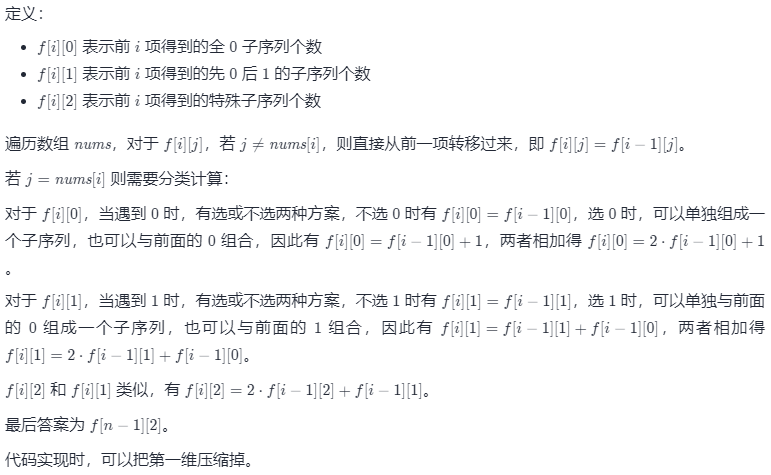
\includegraphics[width=.9\linewidth]{./pic/specialSeq.png}

\begin{minted}[fontsize=\scriptsize,linenos=false]{csharp}
public int countSpecialSubsequences(int[] arr) { // 去找个降维的参考一下
    int mod = (int)1e9 + 7;
    int n = arr.length;
    long [][] dp = new long [n][3];
    for (int i = 0; i < n; i++) 
        for (int j = 0; j < 3; j++) {
            if (arr[i] != j) dp[i][j] = (i == 0 ? 0 : dp[i-1][j]);
            else 
                if (j == 0)
                    dp[i][j] = (i == 0 ? 0 : dp[i-1][j]) * 2 % mod + 1;
                else
                    dp[i][j] = ((i == 0 ? 0 : dp[i-1][j]) * 2 % mod + (i == 0 ? 0 : dp[i-1][j-1])) % mod;
        }
    return (int)dp[n-1][2];
}
\end{minted}

\subsection{446. Arithmetic Slices II - Subsequence - Hard}
\label{sec-1-4-59}
Given an integer array nums, return the number of all the arithmetic subsequences of nums.

A sequence of numbers is called arithmetic if it consists of at least three elements and if the difference between any two consecutive elements is the same.

For example, [1, 3, 5, 7, 9], [7, 7, 7, 7], and [3, -1, -5, -9] are arithmetic sequences.
For example, [1, 1, 2, 5, 7] is not an arithmetic sequence.
A subsequence of an array is a sequence that can be formed by removing some elements (possibly none) of the array.

For example, [2,5,10] is a subsequence of [1,2,1,2,4,1,5,10].
The test cases are generated so that the answer fits in 32-bit integer.
\begin{enumerate}
\item 解题思路与分析
\label{sec-1-4-59-0-1}
这道题是之前那道Arithmetic Slices的延伸,那道题比较简单是因为要求等差数列是连续的,而这道题让我们求是等差数列的子序列,可以跳过某些数字,不一定非得连续,那么难度就加大了,但还是需要用动态规划Dynamic Progrmming来做。

好,既然决定要用DP了,那么首先就要确定dp数组的定义了,刚开始我们可能会考虑使用个一维的dp数组,然后dp[i]定义为范围为[0, i]的子数组中等差数列的个数。定义的很简单,OK,但是基于这种定义的状态转移方程却十分的难想。我们想对于(0, i)之间的任意位置j,如何让 dp[i] 和 dp[j] 产生关联呢?是不是只有 A[i] 和 A[j] 的差值diff,跟A[j]之前等差数列的差值相同,才会有关联,所以差值diff是一个很重要的隐藏信息Hidden Information,我们必须要在dp的定义中考虑进去。所以一维dp数组是罩不住的,必须升维,但是用二维dp数组的话,差值diff那一维的范围又是个问题,数字的范围是整型数,所以差值的范围也很大,为了节省空间,我们建立一个一维数组dp,数组里的元素不是数字,而是放一个HashMap,建立等差数列的差值和当前位置之前差值相同的数字个数之间的映射。我们遍历数组中的所有数字,对于当前遍历到的数字,又从开头遍历到当前数字,计算两个数字之差diff,如果越界了不做任何处理,如果没越界,我们让dp[i]中diff的差值映射自增1,因为此时A[i]前面有相差为diff的A[j],所以映射值要加1。然后我们看dp[j]中是否有diff的映射,如果有的话,说明此时相差为diff的数字至少有三个了,已经能构成题目要求的等差数列了,将dp[j][diff]加入结果res中,然后再更新dp[i][diff],这样等遍历完数组,res即为所求。

我们用题目中给的例子数组 [2,4,6,8,10] 来看,因为2之前没有数字了,所以我们从4开始,遍历前面的数字,是2,二者差值为2,那么在dp\footnotemark[2]{}的HashMap就可以建立 2->1 的映射,表示4之前有1个差值为2的数字,即数字2。那么现在i=2指向6了,遍历前面的数字,第一个数是2,二者相差4,那么在dp\footnotemark[3]{}的HashMap就可以建立 4->1 的映射,第二个数是4,二者相差2,那么先在dp\footnotemark[3]{}的HashMap建立 2->1 的映射,由于dp\footnotemark[2]{}的HashMap中也有差值为2的映射,2->1,那么说明此时至少有三个数字差值相同,即这里的 [2 4 6],我们将dp\footnotemark[2]{}中的映射值加入结果res中,然后当前dp\footnotemark[3]{}中的映射值加上dp\footnotemark[2]{}中的映射值。这应该不难理解,比如当i=3指向数字8时,j=2指向数字6,那么二者差值为2,此时先在dp\footnotemark[4]{}建立 2->1 的映射,由于dp\footnotemark[3]{}中有 2->2 的映射,那么加上数字8其实新增了两个等差数列 [2,4,6,8] 和 [4,6,8],所以结果res加上的值就是 dp[j][diff],即2,并且 dp[i][diff] 也需要加上这个值,才能使得 dp\footnotemark[4]{} 中的映射变为 2->3 ,后面数字10的处理情况也相同,这里就不多赘述了,最终的各个位置的映射关系如下所示:
\begin{minted}[fontsize=\scriptsize,linenos=false]{csharp}
2     4     6     8     10    
     2->1  4->1  6->1  8->1
           2->2  4->1  6->1 
                 2->3  4->2
                       2->4
\end{minted}

最终累计出来的结果是跟上面红色的数字相关,分别对应着如下的等差数列:

\begin{minted}[fontsize=\scriptsize,linenos=false]{csharp}
2->2:[2,4,6]
2->3:[2,4,6,8]    [4,6,8]
4->2:[2,6,10]
2->4:[2,4,6,8,10]    [4,6,8,10]    [6,8,10]
\end{minted}
\begin{itemize}
\item Both time and space complexities are O(n\^{}2)
\end{itemize}

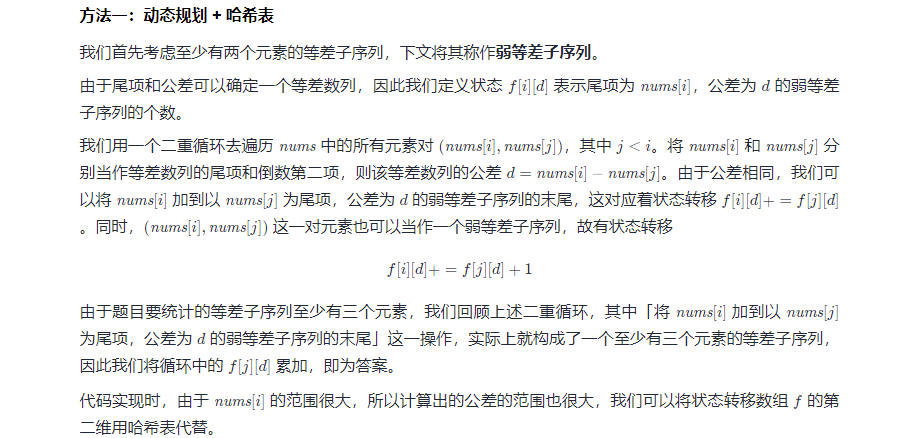
\includegraphics[width=.9\linewidth]{./pic/arithslice.png}

Define the type of the difference as Integer type instead of Long. This is because there is no valid arithmetic subsequence slice that can have difference out of the Integer value range. But we do need a long integer to filter out those invalid cases.

Preallocate the HashMap to avoid reallocation to deal with extreme cases.

Refrain from using lambda expressions inside loops.

\begin{minted}[fontsize=\scriptsize,linenos=false]{csharp}
 public int numberOfArithmeticSlices(int [] a) {
    int n = a.length, ans = 0;
    Map<Integer, Integer> [] dp = new HashMap[n];
    dp[0] = new HashMap<>();
    for (int i = 1; i < n; i++) {
        dp[i] = new HashMap<>();
        for (int j = 0; j < i; j++) {
        // for (int j = i-1; j >= 0; j--) { // BUG: 反向遍历不可以
            long diff = (long)a[i] - a[j];  // bug: (long)a[i]
            if (diff > Integer.MAX_VALUE || diff < Integer.MIN_VALUE) continue;
            int dif = (int)diff;
            dp[i].put(dif, dp[i].getOrDefault(dif, 0) + 1); // bug: 这里加的是1,不是2 // 这里先更新上
            if (dp[j].containsKey(dif)) {
                ans += dp[j].get(dif); // 只自增1(而不是记为2),为的是方便这里统计结果
                dp[i].put(dif, dp[i].get(dif) + dp[j].get(dif));// 再加上之前累积的
            }
        }
    }
    return ans;
}
\end{minted}
\end{enumerate}

\subsection{639. Decode Ways II - Hard}
\label{sec-1-4-60}
A message containing letters from A-Z can be encoded into numbers using the following mapping:

'A' -> "1"
'B' -> "2"
\ldots{}
'Z' -> "26"
To decode an encoded message, all the digits must be grouped then mapped back into letters using the reverse of the mapping above (there may be multiple ways). For example, "11106" can be mapped into:

"AAJF" with the grouping (1 1 10 6)
"KJF" with the grouping (11 10 6)
Note that the grouping (1 11 06) is invalid because "06" cannot be mapped into 'F' since "6" is different from "06".

In addition to the mapping above, an encoded message may contain the '*' character, which can represent any digit from '1' to '9' ('0' is excluded). For example, the encoded message "1*" may represent any of the encoded messages "11", "12", "13", "14", "15", "16", "17", "18", or "19". Decoding "1*" is equivalent to decoding any of the encoded messages it can represent.

Given a string s consisting of digits and '*' characters, return the number of ways to decode it.

Since the answer may be very large, return it modulo 109 + 7.
\begin{enumerate}
\item 解题思路与分析
\label{sec-1-4-60-0-1}
给定一个只含数字的长n nn的字符串s ss,再给定一个对应规则,每个大写字母ch可以对应一个数字ch - 'A' + 1。问该s ss有多少种不同的解码方式。s ss中可能含有'*',这个符号可以对应除了0 00以外的任意一位数。答案模10\^{}9 + 7后返回。

思路是动态规划。设f [ i ] f[i]f[i]是s ss的长i ii的前缀的解码方式数,那么可以按照最后一位(或者两位)是解码成什么字母来分类进行累加。
\begin{minted}[fontsize=\scriptsize,linenos=false]{csharp}
public int numDecodings(String t) {
    int mod = (int)1e9 + 7;
    int n = t.length();
    char [] s = t.toCharArray();
    System.out.println(Arrays.toString(s));
    int [] dp = new int [Math.max(2, n+1)];
    dp[0] = 1;
    dp[1] = s[0] == '*' ? 9 : s[0] == '0' ? 0 : 1;
    for (int i = 2; i <= n; i++) {
        System.out.println("i: " + i);
        for (int j = 1; j <= 26; j++) { // 枚举s的长i前缀的末尾可以解码为哪个大写字母
            char c = s[i-1];
            if (j <= 9) { // 如果是要解码为A到I,那么最后一个数字得单独解码
                if (c == '*' || c == '0' + j)
                    dp[i] += dp[i-1];
            } else {      // 否则最后两个数字得一起解码
                char p = s[i-2];
                int x = j % 10, y = j / 10;
                if ((p == '*' || p == y+ '0') && ((c == '*' && x != 0) || c == x + '0')) 
                    dp[i] += dp[i-2];
            }
            dp[i] %= mod;
        }
    }
    return dp[n];
}
\end{minted}
\item 解题思路与分析
\label{sec-1-4-60-0-2}

定义dp[i]是nums前i个字符可以得到的解码种数,假设之前的字符串是abcx,现在新加入了y,则有以下5种情况:

\begin{minted}[fontsize=\scriptsize,linenos=false]{csharp}
如果x=='0',且y=='0',无法解码,返回0;
如果只有x=='0',则y只能单独放在最后,不能与x合并(不能以0开头),此时有:dp[i] = dp[i-1]
如果只有y=='0',则y不能单独放置,必须与x合并,并且如果合并结果大于26,返回0,否则有:dp[i] = dp[i-2]
如果 xy<=26: 则y可以“单独”放在abcx的每个解码结果之后后,并且如果abcx以x单独结尾,此时可以合并xy作为结尾,而这种解码种数就是abc的解码结果,此时有:dp[i+1] = dp[i] + dp[i-1]
如果 xy>26: 此时x又不能与y合并,y只能单独放在dp[i]的每一种情况的最后,此时有:dp[i+1] = dp[i]
\end{minted}
\begin{minted}[fontsize=\scriptsize,linenos=false]{csharp}
    public int numDecodings(String s) {
        char[] arr = s.toCharArray();
        int[] dp = new int[s.length()+1];
        dp[0] = 1;
        dp[1] = arr[0]=='0'?0:1;
        if(s.length()<=1) return dp[1];
        for(int i=2;i<=s.length();i++){
            int n = (arr[i-2]-'0')*10+(arr[i-1]-'0');
            if(arr[i-1]=='0' && arr[i-2]=='0'){
                return 0;
            }else if(arr[i-2]=='0'){
                dp[i] = dp[i-1];
            }else if(arr[i-1]=='0'){
                if(n>26) return 0;
                dp[i] = dp[i-2];
            }else if(n>26){
                dp[i] = dp[i-1];
            }else{
                dp[i] = dp[i-1]+dp[i-2];
            }
        }
        return dp[dp.length-1];
    }
\end{minted}
\end{enumerate}

\subsection{629. K Inverse Pairs Array - Hard}
\label{sec-1-4-61}
For an integer array nums, an inverse pair is a pair of integers [i, j] where 0 <= i < j < nums.length and nums[i] > nums[j].

Given two integers n and k, return the number of different arrays consist of numbers from 1 to n such that there are exactly k inverse pairs. Since the answer can be huge, return it modulo 109 + 7.
\begin{enumerate}
\item 解题思路与分析
\label{sec-1-4-61-0-1}

比较容易辨别出来是一道DP的题目,但是确实算是比较难的了,下面是参考网上的代码之后我的理解。定义dp[n][k]表示从1到n构成的数中含有k个逆序对的个数,则我们可以推导出dp[n][k]和dp[n - 1][i]之间的递推关系:

如果我们把n放在最后一位,则所有的k个逆序对均来自于前n - 1个数所构成的逆序对,和n无关;

如果我们把n放在倒数第二位,则有1个逆序对和n有关,有k - 1个逆序对来自前n - 1个数所构成的逆序对;

……

如果我们把n放在第一位,则有n-1个逆序对和n有关,k - (n - 1)个逆序对来自前n - 1个数所构成的逆序对。

所以:dp[n][k] = dp[n-1][k]+dp[n-1][k-1]+dp[n-1][k-2]+…+dp[n-1][k+1-n+1]+dp[n-1][k-n+1]。但问题是 k - (n - 1)有可能为负数,也就是说根据n和k的不同,上面的式子有可能从某个项之后就不合法了,我们这里先写出来占位,从而得到下面两个式子:

\begin{minted}[fontsize=\scriptsize,linenos=false]{csharp}
dp[n][k]     = dp[n-1][k] + dp[n-1][k-1] + dp[n-1][k-2] + … + dp[n-1][k + 1-n + 1] + dp[n-1][k-n + 1] // A
dp[n][k + 1] = dp[n-1][k + 1] + dp[n-1][k] + dp[n-1][k-1] + dp[n-1][k-2] + … + dp[n-1][k + 1-n + 1]   // B
dp[n][k+1] - dp[n][k] = dp[n-1][k+1] - dp[n-1][k-n+1]; // B-A           
dp[n][k+1] = dp[n][k] + dp[n-1][k+1] - dp[n-1][k-n+1]; // 移项
// 将k+1换回成k,可以得到:
dp[n][k] = dp[n][k-1] + dp[n - 1][k] - dp[n-1][k-n]
\end{minted}

把上面两个式子相减可以推导出:dp[n][k+1] = dp[n][k]+dp[n-1][k+1]-dp[n-1][k+1-n]。这样就可以写出代码了。

当然由于dp[n][k]只和dp[n][x],dp[n-1][x]有关,所以该代码还可以进一步将空间复杂度从O(nk)降低到O(k)。时间复杂度是O(nk)。

\begin{minted}[fontsize=\scriptsize,linenos=false]{csharp}
public int kInversePairs(int n, int k) {
    int mod = (int)1e9 + 7;
    long [][] dp = new long [n+1][k+1];
    dp[0][0] = 1;
    for (int i = 1; i <= n; i++) {
        dp[i][0] = 1;
        for (int j = 1; j <= k; j++)  {
            dp[i][j] = dp[i][j-1] + dp[i-1][j];
            if (j >= i)
                dp[i][j] -= dp[i-1][j-i];
            dp[i][j] = (dp[i][j] + mod) % mod;
        }
    }
    return (int)dp[n][k];
}
\end{minted}
\item 解题思路与分析
\label{sec-1-4-61-0-2}

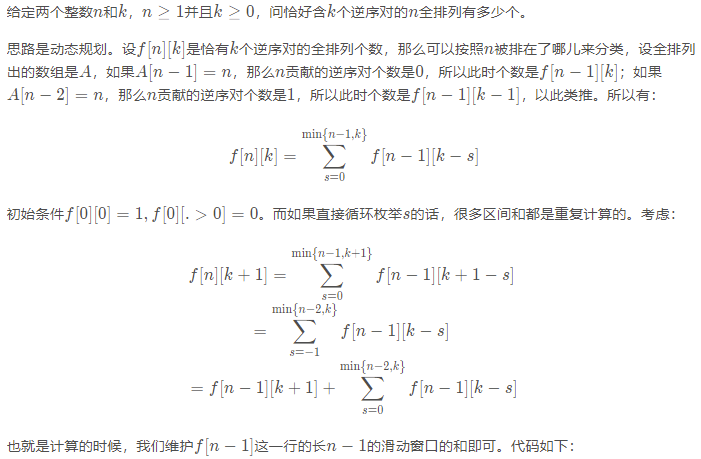
\includegraphics[width=.9\linewidth]{./pic/kinvPair.png}

\begin{minted}[fontsize=\scriptsize,linenos=false]{csharp}
public int kInversePairs(int n, int k) {
    int mod = (int)1e9 + 7;
    int [][] dp = new int [n+1][k+1];
    dp[0][0] = 1;
    for (int i = 1; i <= n; i++) {
        long sum = 0;
        for (int j = 0; j <= k; j++) {
            sum += dp[i-1][j];
            if (j >= i)
                sum -= dp[i-1][j-i];
            dp[i][j] = (int)(sum % mod);
        }
    }
    return (int)dp[n][k];
}
\end{minted}
\end{enumerate}
\subsection{1787. Make the XOR of All Segments Equal to Zero - Hard}
\label{sec-1-4-62}
You are given an array nums​​​ and an integer k​​​​​. The XOR of a segment [left, right] where left <= right is the XOR of all the elements with indices between left and right, inclusive: nums[left] XOR nums[left+1] XOR \ldots{} XOR nums[right].

Return the minimum number of elements to change in the array such that the XOR of all segments of size k​​​​​​ is equal to zero.
\begin{enumerate}
\item 解题思路与分析
\label{sec-1-4-62-0-1}

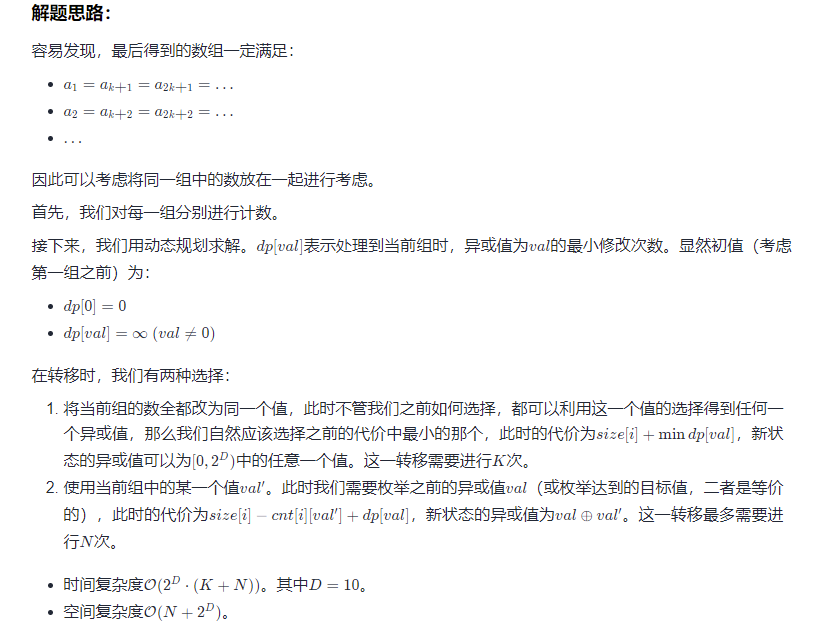
\includegraphics[width=.9\linewidth]{./pic/xortimes.png}

\begin{itemize}
\item 根据题目特点,最后所有长度为 k 的区间异或结果等于零,可推出得到的数组满足:
\end{itemize}
\begin{minted}[fontsize=\scriptsize,linenos=false]{csharp}
a1 = ak+1 = a2k+1 = …
a2 = ak+2 = a2k+2 = …
\end{minted}
因此可将数组中的元素按上述规律,每间隔 k 个的数字为一组进行分组。

在此基础上,设计一个动态规划数组 dp[j],表示到当前第 i 组为止,所有元素异或到对应数字 j 时的更改次数。则对第 i 组 dp[j] 的状态转移方程可能为:

j 可由某一数值和当前组中的某个数 num 异或得到,newDp[j] = dp[j \& num] + size[i] - 组中 num 的数量

j 可通过和任意数字异或得到,newDp[j] = 前一 dp 中最小的改变次数 + size[i]

完成 k 个组的动态规划后,dp\footnotemark[1]{}就是所求的解。

\begin{minted}[fontsize=\scriptsize,linenos=false]{csharp}
public int minChanges(int [] a, int k) {
    int n = a.length;
    Map<Integer, Integer> [] group = new HashMap[k]; // 存储 k 个组、各组中各个数字数量
    int [] cnt = new int [k]; // k元素片段里,每个下标对应的所有元素总个数 // 各组大小,它们会有可能不同吗?
    for (int i = 0; i < k; i++) {
        group[i] = new HashMap<>();
        for (int j = i; j < n; j += k) { // 将数组中的每个元素分布到其在k元素片段中下标位置所在的组里去,并统计重复出现次数
            group[i].put(a[j], group[i].getOrDefault(a[j], 0) + 1);
            cnt[i]++;
        }
    }
    int r = 1 << 10; // 题中nums[i] < 2^10, 为的是遍历所有可能更改值,以取最小
    int [] dp = new int [r], curDp = new int [r]; // 当前组异或到对应数字时的更改次数
    Arrays.fill(dp, Integer.MAX_VALUE);
    dp[0] = 0;
    for (int i = 0; i < k; i++) { // 遍历k个元素的片段——中的每个元素,逐元素优化出全局最优解
        int minVal = Arrays.stream(dp).min().getAsInt(); // 累积到上一个元素的全局最优解
        Arrays.fill(curDp, minVal + cnt[i]); // 变为当前组中不存在数字的改变次数:之前的最小改变次数+当前组元素个数
        for (int j = 0; j < r; j++) {
            if (dp[j] == Integer.MAX_VALUE) continue;
            for (Map.Entry<Integer, Integer> en : group[i].entrySet()) {
                int num = en.getKey(), v = en.getValue(), xorNum = num ^ j;
                curDp[xorNum] = Math.min(curDp[xorNum], dp[j] + cnt[i] - v);
            }
        }
        dp = Arrays.copyOf(curDp, r); // 将遍历到当前组、累积较优解的curDp复制入全局最优解dp数组中
    }
    return dp[0];
}
\end{minted}
\end{enumerate}

\subsection{1735. Count Ways to Make Array With Product - Hard 乘积为K的质因子数排列组合的总个数: 分解质因子}
\label{sec-1-4-63}
You are given a 2D integer array, queries. For each queries[i], where queries[i] = [ni, ki], find the number of different ways you can place positive integers into an array of size ni such that the product of the integers is ki. As the number of ways may be too large, the answer to the ith query is the number of ways modulo 109 + 7.

Return an integer array answer where answer.length == queries.length, and answer[i] is the answer to the ith query.

\begin{enumerate}
\item 解题思路与分析
\label{sec-1-4-63-1}

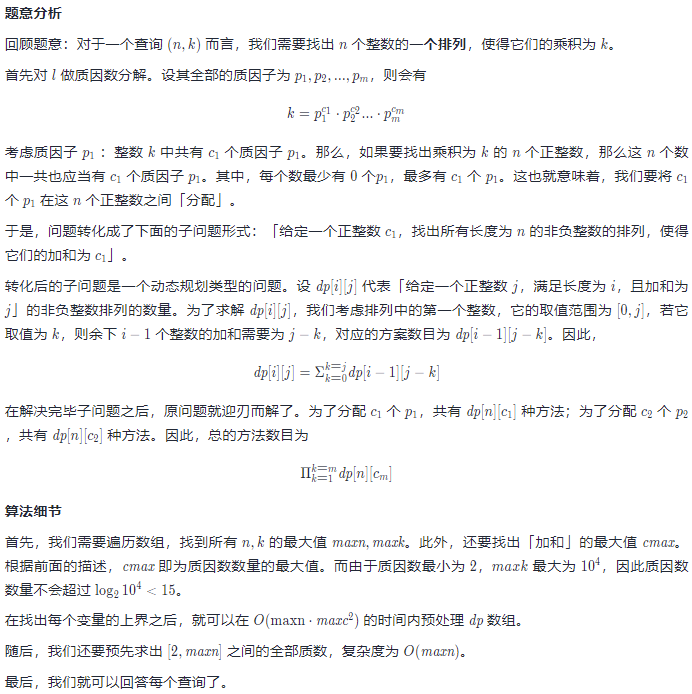
\includegraphics[width=.9\linewidth]{./pic/1735.png}

\begin{minted}[fontsize=\scriptsize,linenos=false]{csharp}
// 在找出每个变量的上界之后,就可以在O(maxn}{maxc}^2)的时间内预处理dp 数组。
//     随后,我们还要预先求出 [2, maxn] 之间的全部质数,复杂度为 O(maxn)。
public int[] waysToFillArray(int[][] q) {
    int n = q.length;
    int mod = (int)1e9 + 7;
    int maxC = 15;          // 找出「加和」的最大值cmax。根据前面的描述,cmax 即为质因数数量的最大值。
    int maxN = 0, maxK = 0; // 而由于质因数最小为 22,maxkmaxk 最大为 10^4因此质因数数量不会超过log_2 10^4 < 15
    for (int i = 0; i < n; i++) { // 需要遍历数组,找到所有 n, kn,k 的最大值maxn,maxk
        maxN = Math.max(maxN, q[i][0]);
        maxK = Math.max(maxK, q[i][1]);
    }
    long [][] dp = new long [maxN + 1][maxC + 1]; // dp[i][j] 代表给定一个正整数 jj,满足长度为 ii,且加和为 jj的非负整数排列的数量。
    for (int i = 1; i <= maxC; i++) 
        dp[1][i] = 1;
    for (int i = 1; i <= maxN; i++) 
        dp[i][0] = 1;
    for (int i = 2; i <= maxN; i++) 
        for (int j = 1; j <= maxC; j++) 
            for (int k = 0; k <= j; k++) { // 为了求解dp[i][j],我们考虑排列中的第一个整数,它的取值范围为 [0,j][0,j],
                dp[i][j] += dp[i-1][j-k];  // 若它取值为 kk,则余下 i-1i−1 个整数的加和需要为 j-kj−k,对应的方案数目为dp[i−1][j−k]
                dp[i][j] %= mod;
            }
    int [] isPrime = new int [maxK + 1]; // 分解乘积的质因子
    Arrays.fill(isPrime, 1);
    List<Integer> primes = new ArrayList<>();
    for (int i = 2; i <= maxK; i++) {
        if (isPrime[i] == 1) 
            primes.add(i);
        for (int j = i*2; j <= i*i && j <= maxK; j += i) // 最大乘积为maxK的数组,分解出小的质因子了,那么凡是小质因子的乘积倍数的数都不是质数
            isPrime[j] = 0;
    }
    int [] ans = new int [n];
    for (int i = 0; i < n; i++) {
        int m = q[i][0], k = q[i][1];
        List<Integer> cs = new ArrayList<>(); // 乘积k的质因子表
        for (int p : primes) {
            if (p > k) break;
            int cnt = 0, left = k;
            while (left % p == 0) {
                left /= p;
                cnt++;
            }
            if (cnt > 0) cs.add(cnt); // 乘积k中各质因子的个数(指数)
        }
        long res = 1;
        for (int c : cs) {
            res *= dp[m][c]; // 数组长度为n,数组和为质因子c的指数个数的所有可能的分布数合数,各质因子之间个数之间相乘
            res %= mod;
        }
        ans[i] = (int)res;
    }
    return ans;
}
\end{minted}
\begin{itemize}
\item 下面这种方法理解得还不是很透
\end{itemize}
\begin{minted}[fontsize=\scriptsize,linenos=false]{csharp}
public int[] waysToFillArray(int[][] queries) {
    int[] result = new int[queries.length];
    int resultIdx = 0;
    Combination combination = new Combination(10030, 20);
    for (int[] q : queries) {
        int n = q[0]; // 长度为n
        int k = q[1]; // 乘积为k
        long product = 1L;
        for (int power : getPrimeFactors(k).values()) {
            // power个球,分到n个位置,每个位置可以为空
            // 等价于:(power+n)个球,分到n个位置,每个位置不能为空  
            // Why? 等价后得到一种分法,每组减去1,就是原来的解
            // 插板法可得 C(power + n - 1, n - 1) = C(power + n - 1, power)
            product = (product * combination.get(n + power - 1, power)) % mod;
        }
        result[resultIdx++] = (int)(product);
    }
    return result;
}
long mod = (int)1e9 + 7;
public HashMap<Integer, Integer> getPrimeFactors(int n) {
    HashMap<Integer, Integer> map = new HashMap();
    for(int i = 2; i <= n; i++) {
        if (n % i == 0) {
            int cnt = 0;
            while (n % i == 0) {
                cnt++;
                n = n / i;
            }
            map.put(i, cnt);
        }
    }
    return map;
}
class Combination {
    long[][] c;
    Combination (int n, int m) {
        c = new long[n + 1][m + 1];
        c[0][0] = 1;
        for(int i = 1; i <= n; i++){
            c[i][0] = 1;
            for(int j = 1; j <= m; j++) 
                c[i][j] = (c[i-1][j-1] + c[i-1][j]) % mod;
        }
    }
    public long get(int n, int m) {
        return c[n][m];
    }
}
\end{minted}
\end{enumerate}

\subsection{1359. Count All Valid Pickup and Delivery Options - Hard}
\label{sec-1-4-64}
Given n orders, each order consist in pickup and delivery services. 

Count all valid pickup/delivery possible sequences such that delivery(i) is always after of pickup(i). 

Since the answer may be too large, return it modulo 10\^{}9 + 7.
\begin{enumerate}
\item 解题思路与分析
\label{sec-1-4-64-0-1}

就是总共有2N个位置,每次放一两个,还剩下多少个位置可以合理占用

\begin{minted}[fontsize=\scriptsize,linenos=false]{csharp}
public int countOrders(int n) {
    int mod = (int)1e9 + 7;
    int spots = n * 2;
    long ans = 1;
    for (int i = n; i >= 2; i--) {
        ans = (ans * spots * (spots - 1) / 2l) % mod;
        spots -= 2;
    }
    return (int)ans;
}
\end{minted}
\end{enumerate}

\subsection{1187. Make Array Strictly Increasing - Hard 需要重写}
\label{sec-1-4-65}
Given two integer arrays arr1 and arr2, return the minimum number of operations (possibly zero) needed to make arr1 strictly increasing.

In one operation, you can choose two indices 0 <= i < arr1.length and 0 <= j < arr2.length and do the assignment arr1[i] = arr2[j].

If there is no way to make arr1 strictly increasing, return -1.
\begin{enumerate}
\item 解题思路与分析
\label{sec-1-4-65-1}
\begin{minted}[fontsize=\scriptsize,linenos=false]{csharp}
public int makeArrayIncreasing(int[] a, int[] b) {
    b = Arrays.stream(b).distinct().toArray();
    Arrays.sort(b);
    int m = a.length, n = b.length;
    int minCnt = 0, minVal = 0;
    Queue<int []> q = new LinkedList<>();
    q.offer(new int [] {-1, 0}); // 初始化,假想第0位的前一位是-1
    for (int i = 0; i < m; i++) {
        minCnt = Integer.MAX_VALUE;
        for (int size = q.size()-1; size >= 0; size--) {
            int [] cur = q.poll(); // 取前一位的一个选择
            if (a[i] > cur[0]) minCnt = Math.min(minCnt, cur[1]); // 先不急将当前选择加入queue中,找到最小的再说
            minVal = binarySearchMin(b, cur[0]); // 查找一个比前一个数大的最小数
            if (minVal != -1) q.offer(new int [] {minVal, cur[1] + 1}); // 将这个最小数加入到queue中,操作次数在前一位的基础上加一
         }
        if (minCnt != Integer.MAX_VALUE) // 如果当前位可以保持不变,将最小次数加入到queue中
            q.offer(new int [] {a[i], minCnt}); 
    }
    if (q.size() == 0) return -1; // 如果最后一位没有合法的选择方案,返回-1
    int ans = Integer.MAX_VALUE;
    while (!q.isEmpty()) ans = Math.min(ans, q.poll()[1]);
    return ans;
}
private int binarySearchMin(int [] arr, int v) {
    int l = 0, r = arr.length-1, m = 0;
    while (l < r) { // l,r: [0, 1]
        m = l + (r-l) / 2;
        if (arr[m] <= v) l = m+1;
        else r = m;
    }
    return arr[l] > v ? arr[l] : -1; // 所以这里要再判断一下
}
\end{minted}
\item 解题思路与分析
\label{sec-1-4-65-2}

这里若是要替换后面的数字为较大的数字,那么就需要在 arr2 中找到比当前数字大的数字,为了让整个数组更容易的递增,那么这个较大数应该尽量越小越好,所以就是要找到第一个比当前数字大的数。为了更容易的在 arr2 中查找,而不是每次都遍历整个数组,需要给 arr2 排个序,然后用二分搜索来查找更高效一些,这里也可以将 arr2 放到一个 TreeSet 中,利用其自动排序的特点,之后再进行二分搜索就行了。这道题的正确解法是用动态规划 Dynamic Programming,这里的 dp 表达式比较难想,一般来说,dp 值都是定义为题目中要求的值,而这道题是个例外,这里的 dp[i][j] 表示对于数组中的前j个数字组成的子数组中,需要替换i次可以使得其变为严格递增,且第j个数字的最小值为 dp[i][j]。这里的 dp 值不是定义为替换次数,而是第j个数字的最小值(可能是替换后的值),因为要保证数组严格递增,最后一个数字的大小很重要,这是个关键信息,而这个数字的大小跟数组坐标之间没有啥必然联系,所以这个信息不太好放到 dp 数组的坐标中,而所求的替换次数跟数组长度是相关的,因为其不可能超过数组的总长度,最差的情况也就是将整个 arr1 数组都替换了(当然还需要考虑 arr2 的长度)。

接下来就来考虑状态转移方程怎么写,由于这里的j表示前j个数字,那么第j个数字实际上是 arr1[j-1],若第j个数字大于 dp[i][j-1],这里表示对于前 j-1 个数字,替换i次可以使得其严格递增,且第 j-1 个数字为 dp[i][j-1],这样的话就不需要额外的替换操作,还是严格递增增的,则 dp[i][j] 可以赋值为 arr1[j-1]。若此时i大于0,说明之前已经进行过替换操作,则上一个操作状态是 dp[i-1][j-1],当前操作是从 arr2 中选一个数字替换 arr1 的第j个数字,这里就要在 arr2 中选择第一个大于 dp[i-1][j-1] 的数字,若存在的话,就用这个数字来更新 dp[i][j] 的值。若某个时刻j等于n了,说明已经到 arr1 的末尾了,若此时 dp[i][j] 不等于 INT\_MAX(初始值),说明是可以将整个 arr1 替换成严格递增的数组的,替换次数就是i,直接返回即可。最终循环退出了,返回 -1,参见代码如下:
\begin{minted}[fontsize=\scriptsize,linenos=false]{cpp}
int makeArrayIncreasing(vector<int>& arr1, vector<int>& arr2) {
    int n = arr1.size();
    if (n == 1) return 0;
    set<int> st(arr2.begin(), arr2.end());
    vector<vector<int>> dp(n + 1, vector<int>(n + 1, INT_MAX));
    dp[0][0] = INT_MIN;
    for (int j = 1; j <= n; ++j) {
        for (int i = 0; i <= j; ++i) {
            if (arr1[j - 1] > dp[i][j - 1]) {
                dp[i][j] = arr1[j - 1];
            }
            if (i > 0) {
                auto it = st.upper_bound(dp[i - 1][j - 1]);
                if (it != st.end()) dp[i][j] = min(dp[i][j], *it);
            }  
            if (j == n && dp[i][j] != INT_MAX) return i;
        }
    }
    return -1;
}
\end{minted}
\end{enumerate}

\section{多维数个数、数种类数 多一维k介入的 dp[i][j][k]}
\label{sec-1-5}
\subsection{920. Number of Music Playlists - Hard}
\label{sec-1-5-1}
Your music player contains n different songs. You want to listen to goal songs (not necessarily different) during your trip. To avoid boredom, you will create a playlist so that:

Every song is played at least once.
A song can only be played again only if k other songs have been played.
Given n, goal, and k, return the number of possible playlists that you can create. Since the answer can be very large, return it modulo 109 + 7.
\begin{enumerate}
\item 解题思路与分析
\label{sec-1-5-1-1}

当加入的是一首新歌,则表示之前的 L-1 首歌中有 j-1 首不同的歌曲,其所有的组合情况都可以加上这首新歌,那么当前其实有 N-(j-1) 首新歌可以选。

当加入的是一首重复的歌,则表示之前的 L-1 首歌中已经有了 j 首不同的歌,那么若没有K的限制,则当前有 j 首重复的歌可以选。但是现在有了K的限制,意思是两首重复歌中间必须要有K首其他的歌,则当前只有 j-K 首可以选。而当 j<k 时,其实这种情况是为0的。<="" li="" >

综上所述可以得到状态转移方程:

\begin{minted}[fontsize=\scriptsize,linenos=false]{csharp}
            dp[i-1][j-1]*(N-(j-1)) + dp[i-1][j]*(j-k)    (j > K)	
           /	
dp[i][j] = 	
           \	
            dp[i-1][j-1] x (N-(j-1))   (j <= K)
\end{minted}
\begin{minted}[fontsize=\scriptsize,linenos=false]{csharp}
public int numMusicPlaylists(int n, int goal, int k) {
    long mod = (int)1e9 + 7;
    long [][] dp = new long [goal+1][n+1]; // dp[i][j]: 播完i首用了j首不同的曲子,分第i首播不播第j首两种情况 (i >= j for sure)
    for (int i = 1; i <= goal; i++) 
        for (int j = 1; j <= n; j++) {
            if (i < j) dp[i][j] = 0; // 这行不能省略   
            else if (i == 1 && j == 1) dp[i][j] = n; // 用1首歌放完1次,共有n种不同的选择
            else if (i > 1 && j == 1) {
                if (k == 0) dp[i][j] = n; // 相当于没有任何外加限制条件
                // else dp[i][1] = 0;     // 这行可略
            } else // 分两种情况: 第i首不播第j首歌(那么可以从前面j-k首里面选择一首),和第i首播第j首歌(第j首就可以从不曾播放过的n-(j-1)首里面选择一首播放)
                dp[i][j] = (dp[i-1][j] * Math.max(j-k, 0) + (j == 0 ? 0 : dp[i-1][j-1] * (n - (j-1)))) % mod;
        }
    return (int)dp[goal][n];
}
\end{minted}
\begin{itemize}
\item 简化一下代码
\end{itemize}
\begin{minted}[fontsize=\scriptsize,linenos=false]{csharp}
static final int mod = (int)1e9 + 7;
public int numMusicPlaylists(int n, int goal, int k) {
    long [][] dp = new long [goal+1][n+1]; // dp[i][j]: 播完i首用了j首不同的曲子,分第i首播不播第j首两种情况 (i >= j for sure)
    dp[0][0] = 1;
    for (int i = 1; i <= goal; i++) 
        for (int j = 1; j <= n; j++) {
            dp[i][j] = (dp[i-1][j-1] * (n - (j-1))) % mod; // 第j首放新歌
            if (j > k)                                     // 第j首放(j-k)之前的某首歌
                dp[i][j] = (dp[i][j] + dp[i-1][j] * (j-k)) % mod;
        }
    return (int)dp[goal][n];
}
\end{minted}
\end{enumerate}

\subsection{1866. Number of Ways to Rearrange Sticks With K Sticks Visible - Hard}
\label{sec-1-5-2}
There are n uniquely-sized sticks whose lengths are integers from 1 to n. You want to arrange the sticks such that exactly k sticks are visible from the left. A stick is visible from the left if there are no longer sticks to the left of it.

For example, if the sticks are arranged [1,3,2,5,4], then the sticks with lengths 1, 3, and 5 are visible from the left.
Given n and k, return the number of such arrangements. Since the answer may be large, return it modulo 109 + 7.
\begin{minted}[fontsize=\scriptsize,linenos=false]{csharp}
// dp[i][j] 表示前面i根木棍可以看到j根
// 设 dp[i][j] 表示从高度为 1, 2, ..., i 的木棍中,高度逐渐递减地插入新的木棍,从左侧看恰好看到 k 根木棍的方案数。
// 后面说看到ith根,不是指从小到大的第ith根棍子,而是指ith这个位置上的棍子
// 如果可以看到ith根的话,那么数量为dp[i-1][j-1]
// 如果看不到ith的话,那么取前面(i-1)里面任意一个出来放在ith的最后,接下来就是从前面i-1个棍子里面看到j根,所以结果是 (i-1)* dp[i-1][j]
public int rearrangeSticks(int n, int k) {
    int mod = (int)1e9 + 7;
    long [][] dp = new long [n+1][k+1];
    dp[0][0] = 1;
    for (int i = 1; i <= n; i++) 
        for (int j = 1; j <= k; j++) 
            dp[i][j] = (dp[i-1][j-1] + (i - 1) * dp[i-1][j]) % mod;
    return (int)dp[n][k];
}
\end{minted}
\begin{itemize}
\item dfs + memo
\end{itemize}
\begin{minted}[fontsize=\scriptsize,linenos=false]{csharp}
public int rearrangeSticks(int n, int k) {
    dp = new long [n+1][k+1];
    return (int)dfs(n, k);
}
int mod = (int)1e9 + 7;
long [][] dp;
private long dfs(int n, int k) {
    if (n < k || k == 0) return 0;
    if (n == k) return 1;
    if (dp[n][k] != 0) return dp[n][k];
    // instead of iterating for every stick
    // we are just multiplying number of ways with (n - 1)
    return dp[n][k] = (dfs(n-1, k-1) + (n - 1) * dfs(n-1, k)) % mod;
}
\end{minted}

\subsection{1916. Count Ways to Build Rooms in an Ant Colony - Hard}
\label{sec-1-5-3}
You are an ant tasked with adding n new rooms numbered 0 to n-1 to your colony. You are given the expansion plan as a 0-indexed integer array of length n, prevRoom, where prevRoom[i] indicates that you must build room prevRoom[i] before building room i, and these two rooms must be connected directly. Room 0 is already built, so prevRoom\footnotemark[1]{} = -1. The expansion plan is given such that once all the rooms are built, every room will be reachable from room 0.

You can only build one room at a time, and you can travel freely between rooms you have already built only if they are connected. You can choose to build any room as long as its previous room is already built.

Return the number of different orders you can build all the rooms in. Since the answer may be large, return it modulo 109 + 7.

对每个节点,可根据所有以其子节点为根的树的节点及排列数量,计算出以当前节点为根的树的节点及排列数量。

本题求解过程涉及较多前置知识点,包括排列组合、乘法逆元、快速乘方等

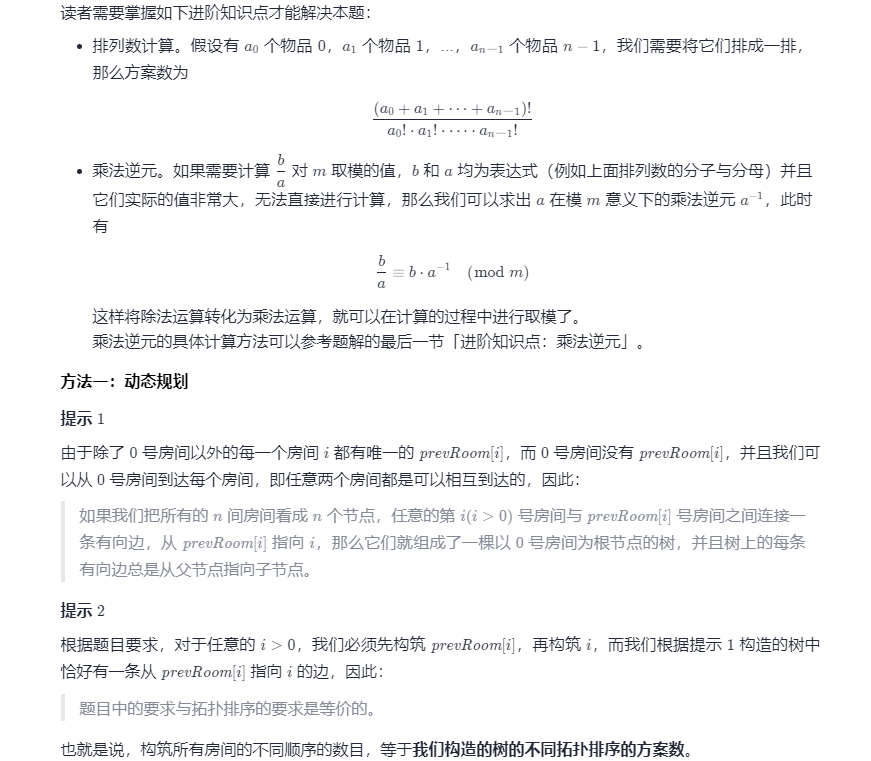
\includegraphics[width=.9\linewidth]{./pic/ant1.png}

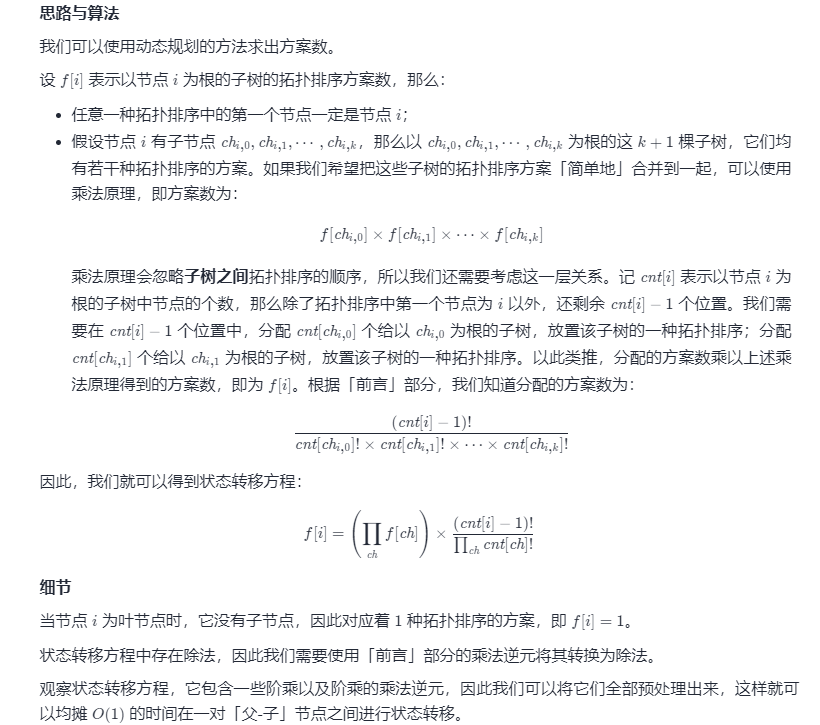
\includegraphics[width=.9\linewidth]{./pic/ant2.png}

\begin{minted}[fontsize=\scriptsize,linenos=false]{csharp}
static final int mod = (int)1e9 + 7;
public int waysToBuildRooms(int[] prevRoom) {
    int n = prevRoom.length;
    // 求阶乘数列及对应逆元
    this.fac = new int [n]; // fac[i]=i!
    this.inv = new int [n]; // inv[i]=i!^(-1)
    fac[0] = inv[0] = 1;
    for (int i = 1; i < n; i++) {
        fac[i] = (int)((long)fac[i-1] * i % mod); // 算阶层
        inv[i] = quickMultiply(fac[i], mod - 2);  // 乘法逆元:费马小定理 : (fac[i]^(-1))%mod = (fac[i]^(mod-2))%mod 转换成快速幂操作
    }
    for (int i = 0; i < n; i++) // 记录各个节点与子节点之间的边
        m.computeIfAbsent(prevRoom[i], z -> new ArrayList<>()).add(i);
    return dfs(0)[1]; // 动态规划得到总体顺序数量x
}
Map<Integer, List<Integer>> m = new HashMap<>();
int [] fac, inv;  
private int [] dfs(int idx) { // 返回以当前节点为根的子树节点个数 及 内部排列数
    if (!m.containsKey(idx)) return new int [] {1, 1}; // 子节点,节点个数及内部排列数均为1
    int cnt = 1, ans = 1; // 子树的结点个数、内部排列数
    for (Integer next : m.get(idx)) {
        int [] cur = dfs(next); // 递归得到子节点对应树的节点个数和排列数
        cnt += cur[0];
        ans = (int)((long)ans * cur[1] % mod * inv[cur[0]] % mod);
    }
    ans = (int)((long)ans * fac[cnt-1] % mod);
    return new int [] {cnt, ans} ;
}
private int quickMultiply(int x, int y) { // 快速幂: 快速计算x^y的乘方
    long ans = 1, base = x;
    while (y > 0) {
        if ((y & 1) == 1)
            ans = (ans * base) % mod; // 指数是奇数次,就先乘一次底数
        base = base * base % mod; // 指数剩偶数次了,就可以直接底数先平方,指数除以2
        y >>= 1; // 指数除2
    }
    return (int) ans;
}
\end{minted}

\subsection{1504. Count Submatrices With All Ones - Medium}
\label{sec-1-5-4}
Given an m x n binary matrix mat, return the number of submatrices that have all ones.
\begin{enumerate}
\item 解题思路与分析
\label{sec-1-5-4-1}

首先我们对矩阵进行数据初始化。即求出每一行以及每一列上的前缀和。

遍历矩阵每一个点(两层循环),并以该点最为起点(row, col),向右下方向画矩形(两层循环,分别循环矩形的宽width和高height),注意矩形范围不能越界。起始时width和height分别为0,即当前点自身是一个矩形。

当width扩大一格后,实际上是增加了(row, col+width)到(row+height, col+width)这一部分的面积(宽为width,高为height),我们通过前缀和数组求出该区域和是否等于height,如果等于,返回结果加一即可。

width扩大一格的操作同理。
\begin{minted}[fontsize=\scriptsize,linenos=false]{csharp}
public int numSubmat(int[][] mat) {
    int m = mat.length, n = mat[0].length;
    int [][] row = new int [m][n]; // 每一行的前缀和
    int [][] col = new int [m][n]; // 每一列的前缀和
    for (int i = 0; i < m; i++)
        for (int j = 0; j < n; j++) 
            row[i][j] = (j == 0 ? 0 : row[i][j-1]) + mat[i][j];
    for (int j = 0; j < n; j++) 
        for (int i = 0; i < m; i++) 
            col[i][j] = (i == 0 ? 0 : col[i-1][j]) + mat[i][j];
    int ans = 0;
    for (int i = 0; i < m; i++) 
        for (int j = 0; j < n; j++) 
            for (int r = 0; i+r < m; r++)       // 以当前点为顶点,向下扩大一格, r = 0 起点是0,当前格自身也是答案
                for (int c = 0; j+c < n; c++) { // 以当前点为顶点,向右扩大一格
                    int x = i + r, y = j + c;
                    // 数新扩张区域内每行每列区域内长度累加和都等于长度,即新增区域每格都是1
                    if ((j == 0 && row[x][y] == c+1 || j > 0 && row[x][y] - row[x][j-1] == c+1)
                        && (i == 0 && col[x][y] == r+1 || i > 0 && col[x][y] - col[i-1][y] == r+1))
                        ans++;
                    else break;
                }
    return ans;
}
\end{minted}
\item 解题思路与分析: 单调栈 todo
\label{sec-1-5-4-2}
\begin{minted}[fontsize=\scriptsize,linenos=false]{csharp}
private int res = 0;
private int n;
public int numSubmat(int[][] mat) {
    this.n = mat[0].length;
    // dp[j] : the height (number of consecutive '1's) of column j 
    int[] dp = new int[n];
    for (int i = 0; i < mat.length; i++) {
        // calculating (updating) heights
        for (int j = 0; j < n; j++) 
            dp[j] = mat[i][j] == 1 ? dp[j] + 1 : 0;
        enumerateRowByMinHeight(dp);
    }
    return res;
}
public void enumerateRowByMinHeight(int[] dp) {
    // monotonic stack storing indices : for index p < q in stack, dp[p] < dp[q]
    Deque<Integer> stack = new LinkedList<>();
    stack.offerLast(-1);
    for (int j = 0; j < n; j++) {
        while (stack.peekLast() != -1 && dp[stack.peekLast()] >= dp[j]) {
            int idx = stack.pollLast();
            res += dp[idx] * (idx - stack.peekLast()) * (j - idx);
        }
        stack.offerLast(j);
    }
    while (stack.peekLast() != -1) {
        int idx = stack.pollLast();
        res += dp[idx] * (idx - stack.peekLast()) * (n - idx);
    }
}
\end{minted}
\begin{minted}[fontsize=\scriptsize,linenos=false]{csharp}
// Used two Arrays to store number of consecutive ones on the left, and number of consecutive ones above(up)
//     In one m*n loop we can count the number of order 1xM rectangles where M belongs to [1,m-1]
//     and we can count rectangles of order MxN each time where M>1. in the k index loop.
public int numSubmat(int[][] mat) {
    int m = mat.length, n = mat[0].length;
    int [][] left = new int [m][n]; // 每一行的前缀和
    int [][] abov = new int [m][n]; // 每一列的前缀和
    int ans = 0;
    for (int i = 0; i < m; i++) 
        for (int j = 0; j < n; j++) 
            if (mat[i][j] == 1)  {
                left[i][j] = (j == 0 ? 0 : left[i][j-1]) + 1;
                ans += (j == 0 ? 1 : left[i][j]);
                abov[i][j] = (i == 0 ? 0 : abov[i-1][j]) + 1;
                if (i > 0) {
                    int min = left[i][j];
                    for (int k = 1; k < abov[i][j]; k++) {
                        min = Math.min(min, left[i-k][j]);
                        ans += min;
                    }
                }
            }
    return ans;
}
\end{minted}
\begin{minted}[fontsize=\scriptsize,linenos=false]{csharp}
// In the first pass through the matrix, we store the heights of 1s above a given i,j
// In the second pass, we go through each element that is nonzero, scan leftwards,
//     adding the minimum of the heights encountered until we reach the beginning of the row or hit a zero.
public int numSubmat(int[][] mat) {
    int m = mat.length, n = mat[0].length;
    for (int j = 0; j < n; j++) {
        int colsum = 0;
        for (int i = 0; i < m; i++) {
            if (mat[i][j] == 0) colsum = 0;
            else colsum += mat[i][j];
            mat[i][j] = colsum;
        }
    }
    int tot = 0;
    for (int i = 0; i < m; i++) 
        for (int j = 0; j < mat[i].length; j++) {
            int k = j;
            int min = Integer.MAX_VALUE;
            while (k >= 0 && mat[i][k] != 0) {
                min = Math.min(min, mat[i][k]);
                tot += min;
                k--;
            }
        }
    return tot;
}
\end{minted}
\end{enumerate}
\subsection{1621. Number of Sets of K Non-Overlapping Line Segments - Medium}
\label{sec-1-5-5}
Given n points on a 1-D plane, where the ith point (from 0 to n-1) is at x = i, find the number of ways we can draw exactly k non-overlapping line segments such that each segment covers two or more points. The endpoints of each segment must have integral coordinates. The k line segments do not have to cover all n points, and they are allowed to share endpoints.

Return the number of ways we can draw k non-overlapping line segments. Since this number can be huge, return it modulo 109 + 7.
\begin{enumerate}
\item 解题思路与分析: dfs记忆化搜索, 很慢很慢很慢。。。。。。
\label{sec-1-5-5-1}
\begin{minted}[fontsize=\scriptsize,linenos=false]{csharp}
public int numberOfSets(int n, int k) { 
    if (k == n-1) return 1;
    this.n = n;
    dp = new Long [n][k+1];
    return (int)dfs(0, k);
}
long mod = (int)1e9 + 7;
Long [][] dp; // have to be Long, Integer overflow
int n;
private long dfs(int idx, int k) {
    if (dp[idx][k] != null) return dp[idx][k];
    if (k == 0) return 1;
    long ans = 0;
    for (int i = idx+1; i < n; i++)
        ans += (i - idx) * dfs(i, k-1);
    return dp[idx][k] = ans % mod;
}
\end{minted}
\item 解题思路与分析: dp[i][j][k]
\label{sec-1-5-5-2}

记 f[i][j]f[i][j] 表示使用 0 .. i 的点构造了 jj 条线段的方案数。我们需要区分第 jj 条线段的右端点是否就是 ii,因此可以考虑把 f[i][j] 拆分成两个状态:

\begin{itemize}
\item f[i][j]\footnotemark[1]{} 表示第 jj 条线段的右端点不是 ii,也就是说我们没有办法继续延长第 jj 条线段;
\item f[i][j]\footnotemark[2]{} 表示第 jj 条线段的右端点就是 ii,也就是说我们可以选择是否继续延长第 jj 条线段。
\end{itemize}

如何进行状态转移呢?

首先考虑 f[i][j]\footnotemark[1]{}f[i][j]\footnotemark[1]{},因为第 jj 条线段的右端点不是 ii,因此第 ii 个点没有用上,那么 0 .. i-1 的点构造了 jj 条线段,即

\begin{itemize}
\item f[i][j]\footnotemark[1]{} = f[i-1][j]\footnotemark[1]{} + f[i-1][j]\footnotemark[2]{}
\end{itemize}

再考虑 f[i][j]\footnotemark[2]{}f[i][j]\footnotemark[2]{},因为第 jj 条线段的右端点就是 ii,因此有两种情况:

第 jj 条线段长度为 11,那么 0 .. i-1 的点构造了 j-1j−1 条线段,即

\begin{itemize}
\item f[i][j]\footnotemark[2]{} = f[i-1][j-1]\footnotemark[1]{} + f[i-1][j-1]\footnotemark[2]{}
\end{itemize}

第 jj 条线段长度大于 11,那么删去第 jj 条线段 i-1 .. i 的这一部分,0 .. i-1 的点仍然构造了 jj 条线段,并且点 i-1i−1 是属于第 jj 条线段的,即

\begin{itemize}
\item f[i][j]\footnotemark[2]{} = f[i-1][j]\footnotemark[2]{}
\end{itemize}

加上边界条件 f\footnotemark[1]{}\textsuperscript{,}\,\footnotemark[1]{}\textsuperscript{,}\,\footnotemark[1]{} = 1,最终答案即为 f[n-1][k]\footnotemark[1]{} + f[n-1][k]\footnotemark[2]{}.

\begin{minted}[fontsize=\scriptsize,linenos=false]{csharp}
public int numberOfSets(int n, int k) {
    int mod = (int)1e9 + 7;
    long [][][] dp = new long [n][k+1][2]; // dp[i][j][0/1]: 0, 1, 2 ... i形成j段线段,并且第j段线段是1(否0)以点i结尾
    dp[0][0][0] = 1;
    for (int i = 1; i < n; i++) {
        for (int j = 0; j <= k; j++) {
            dp[i][j][0] = (dp[i-1][j][0] + dp[i-1][j][1]) % mod;
            dp[i][j][1] = dp[i-1][j][1];
            if (j > 0)
                dp[i][j][1] = (dp[i][j][1] + dp[i-1][j-1][0] + dp[i-1][j-1][1]) % mod; 
        }
    }
    return (int)((dp[n-1][k][0] + dp[n-1][k][1]) % mod);
}
\end{minted}
\item 解题思路与分析: dp[i][j]
\label{sec-1-5-5-3}

dp[i][j] means how many number of ways we cut j segments for first i points. The result will be dp[n - 1][k]

It is easy to come up with O(N * N * K) solutions
\begin{minted}[fontsize=\scriptsize,linenos=false]{csharp}
1. Initial value: dp[0][0] = 1. It is only 1 ways to cut first 0 points to 0 segments.
2. For i > 0, dp[i][j] = dp[i - 1][j]. This is assuming that we don't have jth segment ends up with i th points but j segments can be formed by first i - 1 points.
3. Now lets' handle those cases that j th segment which will ends up with ith points. jth segments length varies.
\end{minted}

dp[i][j] = sum(dp\footnotemark[1]{}[j - 1] \ldots{}.. dp[i - 1][j - 1])

\begin{minted}[fontsize=\scriptsize,linenos=false]{csharp}
int mod = 1_000_000_007;                // tle
public int numberOfSets(int n, int k) { // tle
    long[][] dp = new long[n][k + 1];
    dp[0][0] = 1;
    for (int i = 0; i < n; i++) 
        for (int j = 0; j <= Math.min(k, i); j++) {
            if (i > 0) dp[i][j] = dp[i - 1][j];
            if (j > 0) 
                for (int h = i - 1; h >= 0; h--) 
                    dp[i][j] = (dp[i][j] + dp[h][j - 1]) % mod;
        }
    return (int)dp[n - 1][k];
}
\end{minted}

\begin{itemize}
\item However it won't pass LC, because the time complexity is too high. Let's optimize it. We can see the inner for loop. It counts ALL values of dp[0\ldots{}i - 1][j - 1].
\end{itemize}
\begin{minted}[fontsize=\scriptsize,linenos=false]{csharp}
for (int h = i - 1; h >= 0; h--) 
    dp[i][j] = (dp[i][j] + dp[h][j - 1]) % mod;
\end{minted}

\begin{itemize}
\item We can use a new array to store the previous sum of it. In this way, we don't need compute again. In order to use previous sum, we have to reverse the order of for (int j = 0; j <= Math.min(k, i); j++) to for (int j = Math.min(k, i); j >= 0; j--).
\end{itemize}
\begin{minted}[fontsize=\scriptsize,linenos=false]{csharp}
int mod = 1_000_000_007;
public int numberOfSets(int n, int k) {
    long[][] dp = new long[n][k + 1];
    dp[0][0] = 1;
    long[] sums = new long[k + 1];
    for (int i = 0; i < n; i++) 
        for (int j = Math.min(k, i); j >= 0; j--) {
            if (i > 0) dp[i][j] = dp[i - 1][j];
            if (j > 0) dp[i][j] = (sums[j - 1] + dp[i][j]) % mod;
            sums[j] = (sums[j] + dp[i][j]) % mod;
        }
    return (int)dp[n - 1][k];
}
\end{minted}
\end{enumerate}

\section{BitMask掩码相关的【这是第三次不会的】}
\label{sec-1-6}
\subsection{1595. Minimum Cost to Connect Two Groups of Points}
\label{sec-1-6-1}
You are given two groups of points where the first group has size1 points, the second group has size2 points, and size1 >= size2.

The cost of the connection between any two points are given in an size1 x size2 matrix where cost[i][j] is the cost of connecting point i of the first group and point j of the second group. The groups are connected if each point in both groups is connected to one or more points in the opposite group. In other words, each point in the first group must be connected to at least one point in the second group, and each point in the second group must be connected to at least one point in the first group.

Return the minimum cost it takes to connect the two groups.

\begin{itemize}
\item 主要是,它可能涉及的过程状态狠多,要想全了
\end{itemize}

\begin{minted}[fontsize=\scriptsize,linenos=false]{java}
public int connectTwoGroups(List<List<Integer>> a) { // 看来这个题。。。1595 要好好多想几遍【爱表哥,爱生活!!!】
    int m = a.size(), n = a.get(0).size();
    int [][] r = new int [m][1 << n]; // 这里,就是准备,待用
    for (int i = 0; i < m; i++) {
        for (int j = 0; j < (1 << n); j++) {
            int sum = 0;
            for (int k = 0; k < n; k++)
                if ((j & (1 << k)) > 0) sum += a.get(i).get(k);
            r[i][j] = sum;
        }
    }
    int [][] f = new int [m+1][1 << n];
    Arrays.stream(f).forEach(z -> Arrays.fill(z, Integer.MAX_VALUE));
    // f[0][0] = 0; // 【BUG:】初始化得不对,这里一个点是不行的,得一行点。。。
    f[1] = r[0];
    for (int i = 1; i < m; i++)  // 遍历每一行: 左边的每个点,要么去更新已连的右边点减少销耗,要么去连一个新的点
        // for (int j = (1 << n)-1; j > 0; j--) { // 遍历每一种与右点配对现状的更新可能性
        for (int j = 1; j < (1 << n); j++) {
            // 【更新:】右边现存连点中的每个状态下的每个点,将其换连成左边这个点【仍然不对】。。。。
            for (int k = 0; k < n; k++) { // 遍历右边当前状态 mask 下,每个点,【与左边当前遍历点】的更新可能性【情况二分】
                // if ((j & (1 << k)) > 0) // 当前点连了一个某个左边点:这里遍历的状态,仍然不够,左边这个待连点,仍然是可以与右边一片点,几个狠多个点一起连的。。。
                    // f[i][j | (1 << k)] = Math.min(f[i][j | (1 << k)], f[i-1][j] + a.get(i).get(k));
                    // f[i+1][j] = Math.min(f[i+1][j], f[i][j ^ (1 << k)] + a.get(i).get(k)); // 把右边 k 点,换成连左边 i 点
                    // f[i+1][j | (1 << k)] = Math.min(f[i+1][j | (1 << k)], f[i][j] + a.get(i).get(k)); // 把右边 k 点,换成连左边 i 点

                // else // 【BUG:】出发点是对的,但没想全,就是左边这个点,不是只能连右边一个点,还可以是一片点?所以有狠多状态。。。
                    f[i+1][j | (1 << k)] = Math.min(f[i+1][j | (1 << k)], f[i][j] + a.get(i).get(k));
            }
            // 【更新:】右边还没有连的连点中的每个状态下的每个还没能连的点,将其连接成左边这个点,左边这个点可以对应右边狠多个点连接
            int rest = (1 << n)-1 - j; // 想要表示:右连,所有还不曾被连过的点,所有可能的状态 rest 表示截至第 i 行还没被选过的列
            for (int k = rest; k > 0; k = (k - 1) & rest) // 只遍历没选过的列的所有组合 
                f[i+1][j | k] = Math.min(f[i+1][j | k], f[i][j] + r[i][k]);
                // f[i][j | k] = Math.min(f[i][j | k], f[i-1][j] + r[i][k]);
        }
    // return f[m-1][(1 << n) - 1];
    return f[m][(1 << n) - 1];
}
\end{minted}
\section{【第三次】不会的}
\label{sec-1-7}
\subsection{1187. Make Array Strictly Increasing: 【动规:】思路独特}
\label{sec-1-7-1}
Given two integer arrays arr1 and arr2, return the minimum number of operations (possibly zero) needed to make arr1 strictly increasing.

In one operation, you can choose two indices 0 <= i < arr1.length and 0 <= j < arr2.length and do the assignment arr1[i] = arr2[j].

If there is no way to make arr1 strictly increasing, return -1.

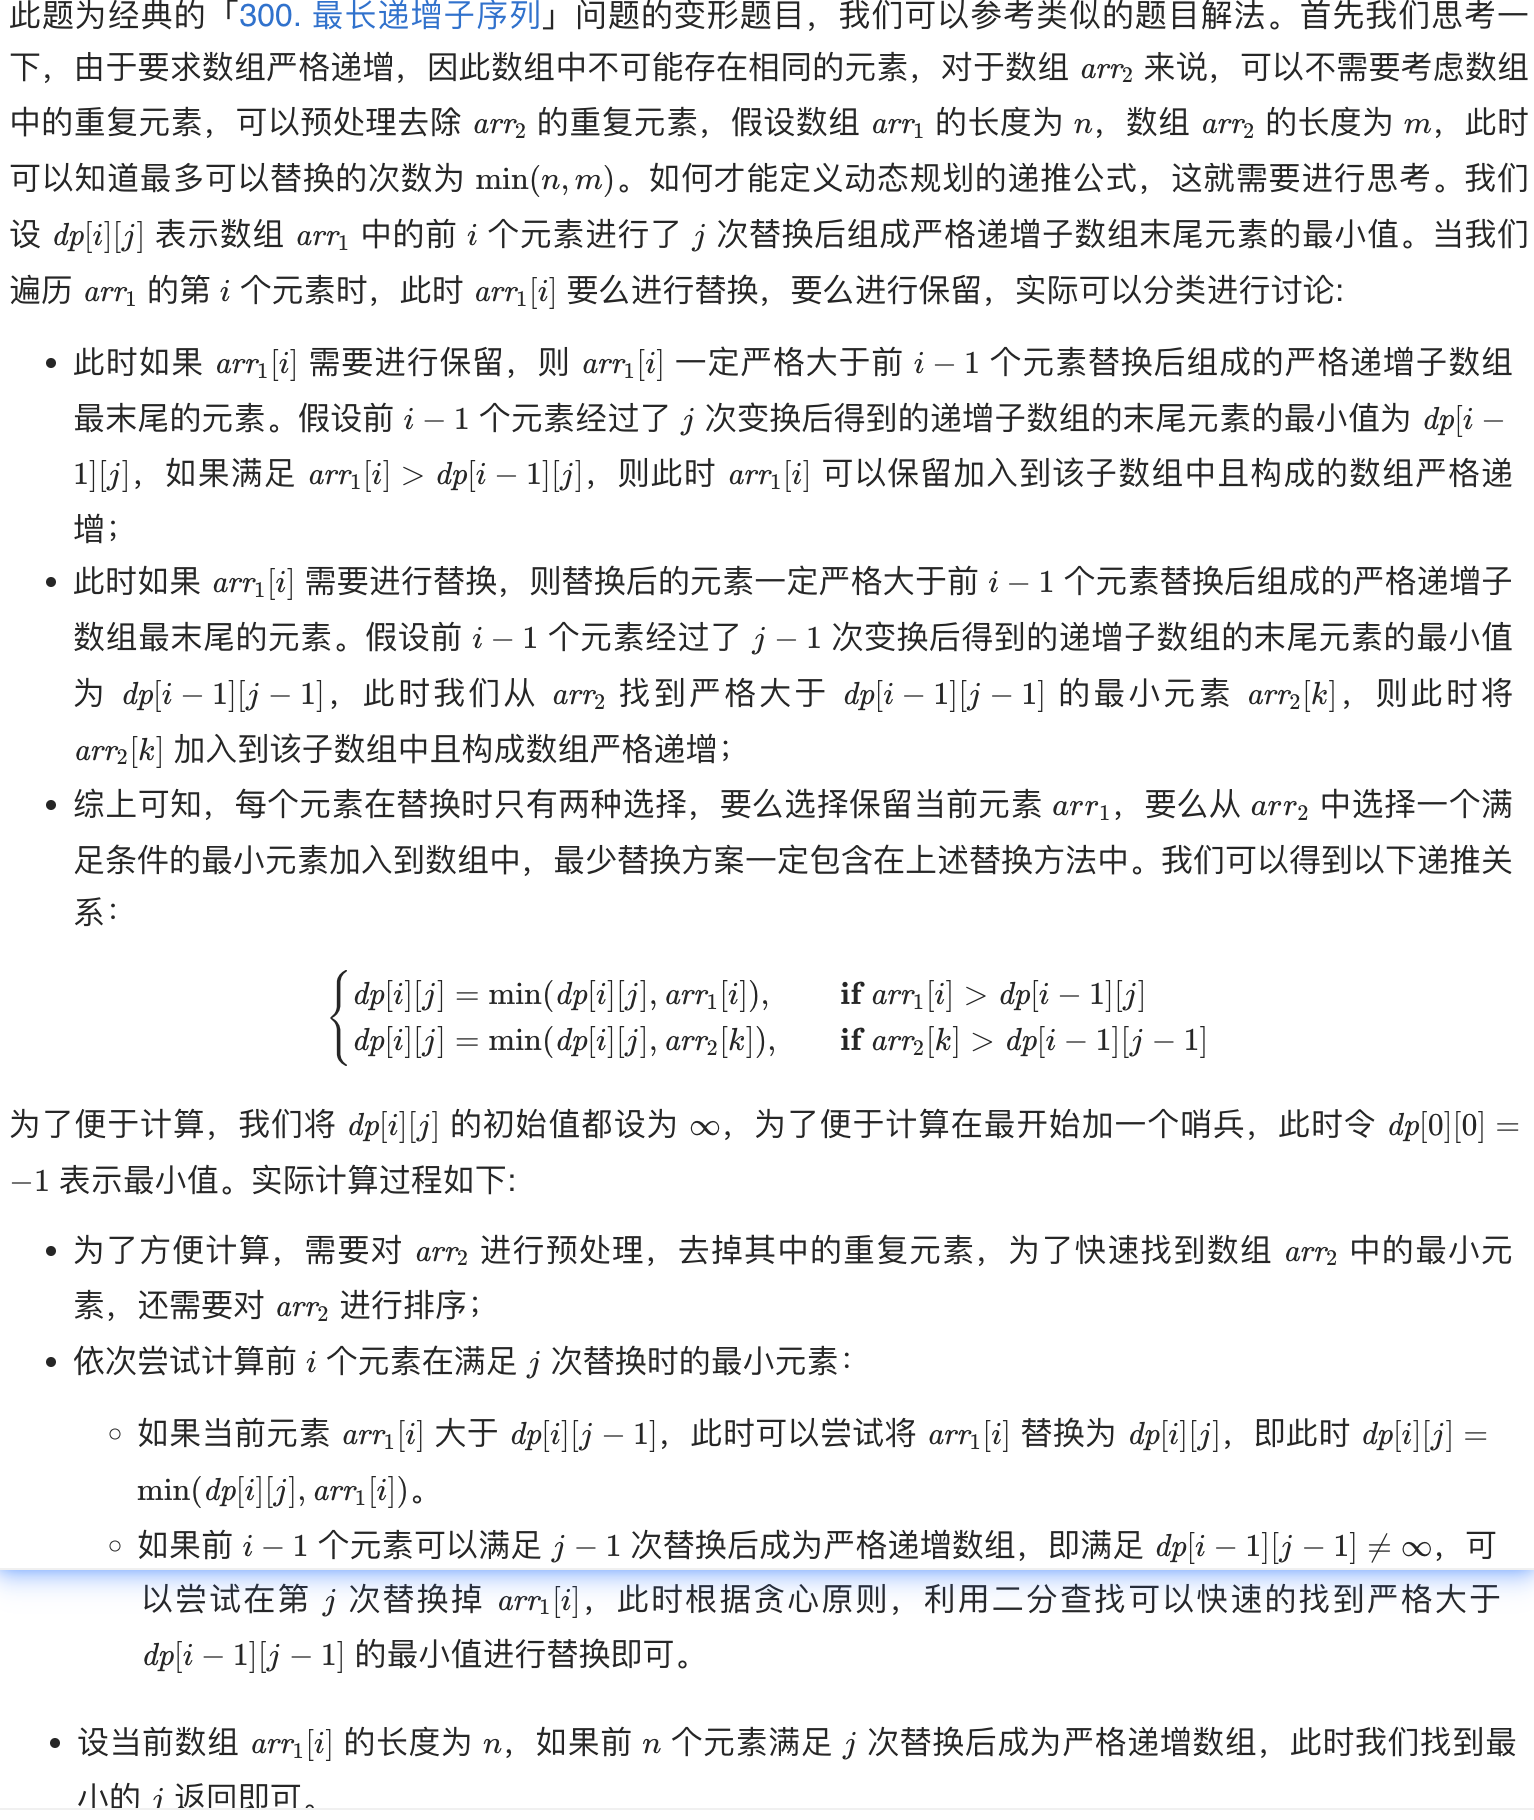
\includegraphics[width=.9\linewidth]{./pic/dp_20230501_092059.png}
\begin{minted}[fontsize=\scriptsize,linenos=false]{java}
public int makeArrayIncreasing(int[] a, int[] b) {
    Arrays.sort(b);
    int n = a.length, p = -1; m = b.length;
    li = new ArrayList<>(); // 尽量写这种简单的,免得自己容易数错
    for (int v : b) {
        if (v != p) li.add(v);
        p = v;
    }
    m = li.size(); 
    int [][] f = new int [n+1][Math.min(m, n) + 1]; // 最多时行 Math.min(m, b) 次交换
    Arrays.stream(f).forEach(z -> Arrays.fill(z, Integer.MAX_VALUE));
    f[0][0] = -1; // 哨兵:-1
    for (int i = 1; i <= n; i++) 
        for (int j = 0; j <= Math.min(i, m); j++) { // 分两种情况来更新
            /* 如果当前元素大于序列的最后一个元素 */
            if (a[i-1] > f[i-1][j])
                f[i][j] = a[i-1];
            /* 查找严格大于 dp[i - 1][j - 1] 的最小元素 */
            if (j > 0 && f[i-1][j-1] != Integer.MAX_VALUE) {
                int idx = binarySearch(j-1, f[i-1][j-1]);
                if (idx != m)
                    f[i][j] = Math.min(f[i][j], li.get(idx));
            }
            if (i == n && f[i][j] != Integer.MAX_VALUE) return j;
        }
    return -1;
}
List<Integer> li;
int m;
int binarySearch(int l, int v) { // 去找第一个 >= v 的下标
    int r = m; // 右边界:不包括【l,r):感觉这里我还没有弄狠透彻。。。
    while (l < r) {
        int mid = (l + r) / 2;
        if (li.get(mid) > v) r = mid;
        else l = mid + 1;
    }
    return l;
}
\end{minted}
\subsection{416. Partition Equal Subset Sum 同硬币和问题,感觉总容易忘记,有点儿提示才能回想起来}
\label{sec-1-7-2}
Given an integer array nums, return true if you can partition the array into two subsets such that the sum of the elements in both subsets is equal or false otherwise.
\begin{enumerate}
\item 动规:二维
\label{sec-1-7-2-1}

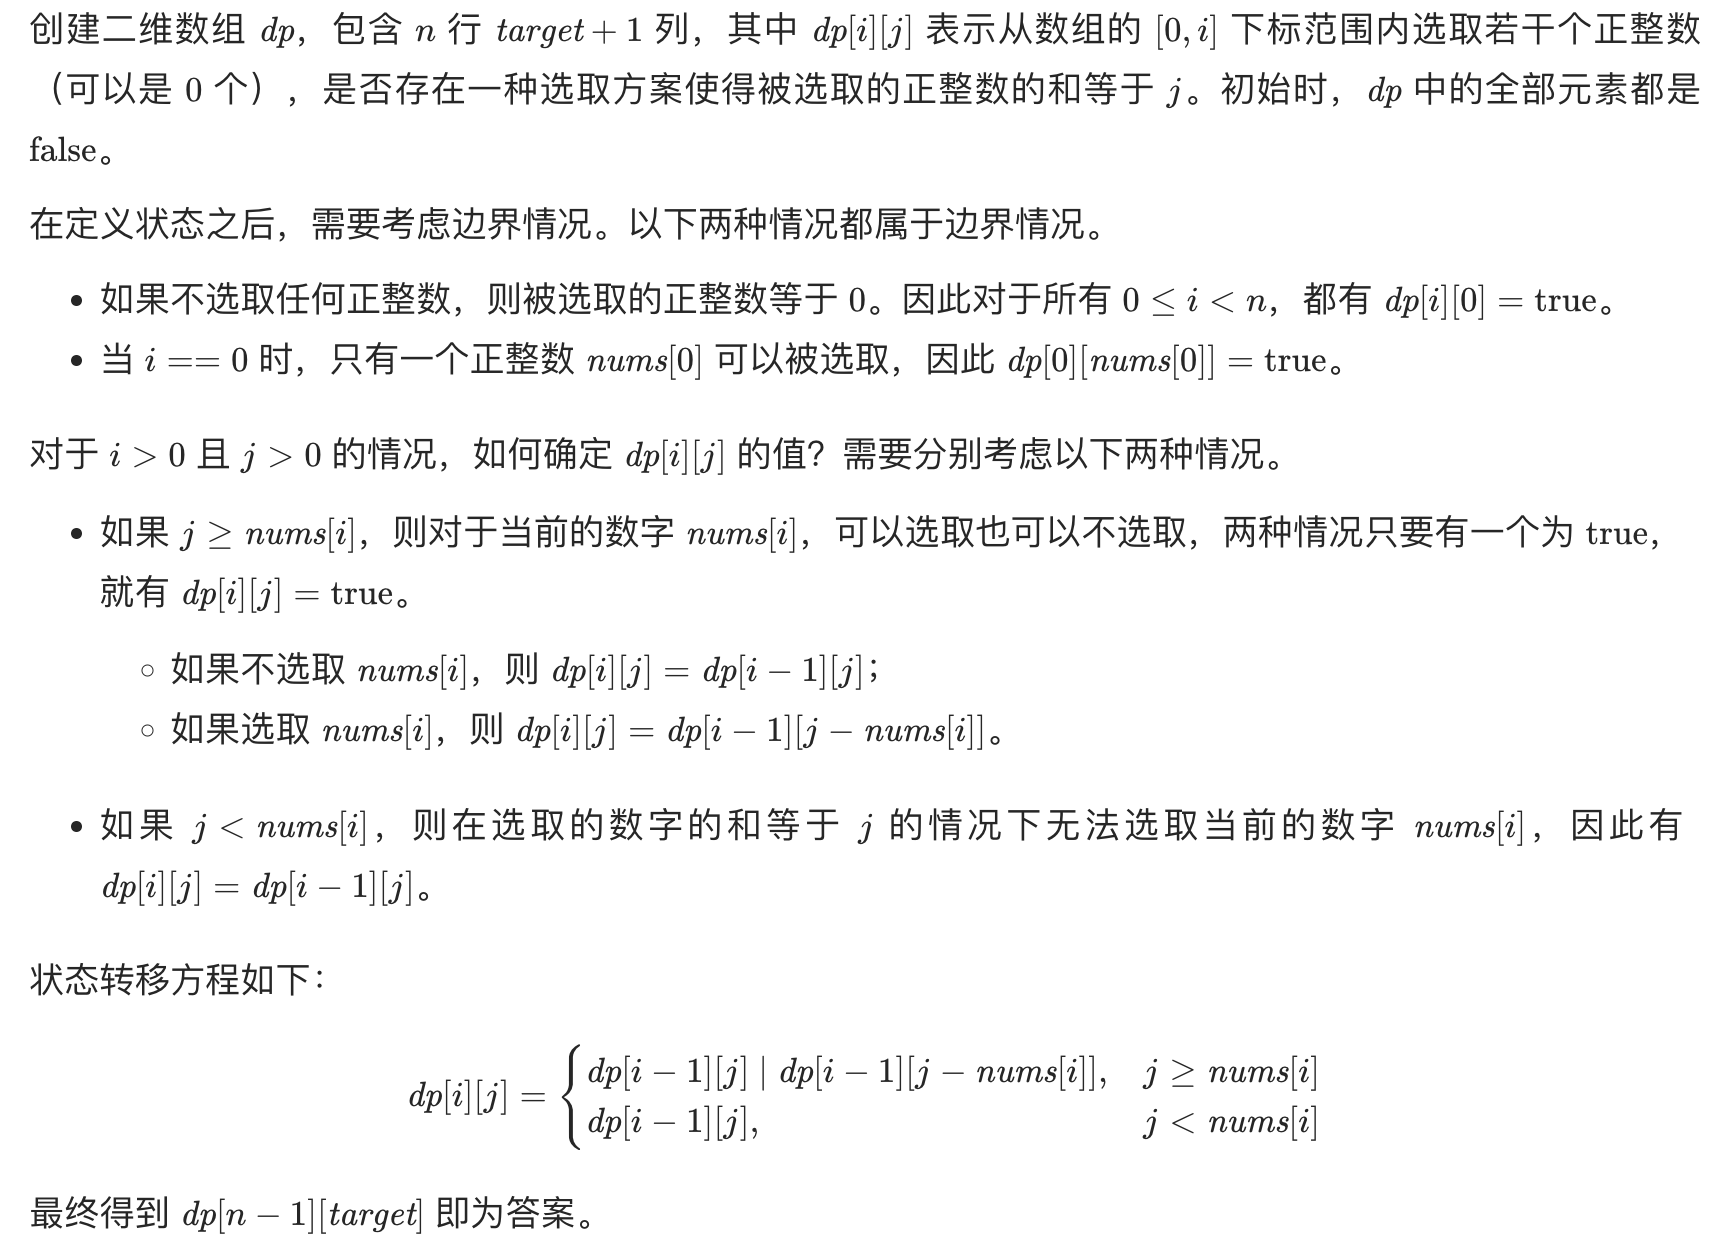
\includegraphics[width=.9\linewidth]{./pic/dp_20230419_141627.png}
\begin{minted}[fontsize=\scriptsize,linenos=false]{java}
// 【动规:】同拼硬币什么之类的题目是一样的. 所以,有了最基本的提醒之后,我是可以自己把它想出来的。。。
public boolean canPartition(int[] a) { // 好慢,还没有上面的,自己瓣出来的一维的快
    int n = a.length;
    if (n < 2) return false;
    int sum = Arrays.stream(a).sum(), max = Arrays.stream(a).max().getAsInt(), target = sum / 2;
    if (sum % 2 != 0 || max > sum / 2) return false;
    Arrays.sort(a); // 子集:之类的,一般顺序不重要,所以解题时,可以排序,来帮助自己解答问题
    boolean [][] f = new boolean [n][target + 1];
    Arrays.stream(f).forEach(z -> Arrays.fill(z, false));
    for (int i = 0; i < n; i++) f[i][0] = true;
    f[0][a[0]] = true;
    for (int i = 1; i < n; i++) {
        int v = a[i];
        for (int j = 1; j <= target; j++) {
            if (j < v) // 因为这些现取得的值 j, 不能通过当前数得到,只能取它们先前只能得到的结果
                f[i][j] = f[i-1][j]; 
            else // 这些取值,就可以通过添加一个当前数 a[i] 取得
                f[i][j] = f[i-1][j] | f[i-1][j-v];
        }
    }
    return f[n-1][target];
}
\end{minted}
\item 动规:一维,压缩空间
\label{sec-1-7-2-2}
\begin{minted}[fontsize=\scriptsize,linenos=false]{java}
public boolean canPartition(int[] a) { // 这里至少也得降序排列一下呀。。。先试着分两组,往什么数组和小的一组里去添加之类的。。。
    int n = a.length;
    if (n < 2) return false;
    int sum = Arrays.stream(a).sum(), max = Arrays.stream(a).max().getAsInt(), target = sum / 2;
    if (sum % 2 != 0 || max > sum / 2) return false;
    Arrays.sort(a); // 子集:之类的,一般顺序不重要,所以解题时,可以排序,来帮助自己解答问题
    boolean [] f = new boolean [target + 1];
    Arrays.fill(f, false);
    f[0] = true;
    // f[a[0]] = true; // 一维时,这个初始化也不必要了。。。
    // for (int i = 1; i < n; i++) {
    for (int i = 0; i < n; i++) {
        int v = a[i];
        for (int j = target; j >= v; j--)
            f[j] |= f[j-v];
    }
    return f[target];
}
\end{minted}
\end{enumerate}
% Emacs 28.2 (Org mode 8.2.7c)
\end{document}